\chapter{生物智能解剖 — 湿件的策略}
\label{chp:biological_intelligence}

本章不再使用模糊神经科学隐喻，而改用\textbf{拓扑旋量、谐振腔、势能面}等物理概念对现实智能系统做解剖对比：从最小细胞单元出发，依次讨论群体智能、颅内智能与更广义的生物智能。

\section{单细胞 (The Cell) : 最小的几何热力学机}
\label{sec:single_cell_anatomy}

智能的过程在多个尺度上呈现出分形式的结构相似性，智能不应仅被视为神经系统的涌现特性。\textbf{细胞 (The Cell)}作为生命的基本单位，可以被视为一种极简的“闭环自维持系统”，其结构要素与本文的 \textbf{Class V (流体智能)} 框架存在可对照的对应关系。

它在微米级的物理空间内，已经具备了 \textbf{边界—介质—核心} 的三体原型，并呈现“激发—演化—坍缩—固化”的循环结构；在本文的叙事中，这可作为 \textbf{全息递归公理} 的一种启发式例证：宏观人脑可以被理解为大量微观闭环单元在更高维度上的耦合投影。基于此，我们可以将单细胞视为一个微型的 \textbf{几何热力学机}（类比）。

\smalltitle{本节内容说明}
\begin{itemize}
    \item \textbf{机制边界}：细胞决策主要由基因调控网络与信号通路的动力学决定；本文将其映射为“宏观算子/势能建筑师”属于结构类比，应避免被误读为细胞具有人类式意向。
    \item \textbf{时间尺度}：膜电位/第二信使为毫秒—秒级，转录-翻译为分钟—小时级；用该分离支撑 $\tau_{field}$ 与 $\tau_{macro}$ 的对应是合理的，但属于粗粒度分层。
    \item \textbf{能量约束}：离子泵与代谢维持的能量预算决定了可用“负熵输入”上限；所有“增益/放大”都必须落在可供能范围内。
\end{itemize}

\smalltitle{微观层 ($L_{micro}$)：细胞膜 (The Membrane) —— VTE 与狄利克雷边界}

细胞膜不仅是物理屏障，更是智能体与环境的\textbf{全息切面}。

\begin{itemize}
    \item   \textbf{狄利克雷边界 (Dirichlet Boundary)}：
    膜通过离子泵维持着细胞内外的电化学梯度（负熵势能）。它将内部的\textbf{生化流形 $\mathcal{M}_{in}$} 与外部的\textbf{环境流形 $\mathcal{M}_{out}$} 强行隔绝，定义了“自我”的物理边界。

    \item   \textbf{VTE 编码器 (Receptors as VTE)}：
    膜上的\textbf{GPCR (G蛋白偶联受体)}或 \textbf{离子通道}充当了变分拓扑编码器。
    \begin{itemize}
        \item   \textbf{输入}：外界混沌的化学汤（噪声）或机械力。
        \item   \textbf{编码}：当特定配体（Ligand）结合时，受体发生构象改变（几何相变），将连续物理输入 $\mathbf{S}_{raw}$（实现层载荷）离散化为内部的 \textbf{第二信使 (Second Messengers)} 或 \textbf{膜电位跳变}。
        \item   \textbf{激波注入}：这是将外部物理量“离散化/内禀化”为可传播的内部激发，并注入内部流形的过程；在本文框架下可类比为“形质基元 (Semantion) 的注入”。
    \end{itemize}
\end{itemize}

\smalltitle{认知场 ($\Psi$)：细胞质 (Cytoplasm) —— 反应-扩散的黎曼流形}

细胞质基质与细胞骨架并非填充物，而是承载信息流动的\textbf{连续介质}。

\begin{itemize}
    \item   \textbf{底流形 ($\mathcal{M}_{cyto}$)}：
    由 \textbf{蛋白相互作用网络 (PPI)} 和 \textbf{细胞骨架 (Cytoskeleton)} 构成的拓扑结构。信号分子并非随机扩散，而是沿着由骨架蛋白铺设的 \textbf{测地线 (Geodesic)} 定向运输。

    \item   \textbf{语义子 ($\Psi$)}：
    被激活的激酶 (Kinases)、钙波 (Calcium Waves)、cAMP 分子。它们是携带信息的能量包，在细胞质这个 \textbf{介质层} 中扩散、干涉。

    \item   \textbf{动力学方程}：
    信号传导遵循 \textbf{反应-扩散方程 (Reaction-Diffusion Equation)}，这是 \textbf{目的论狄拉克方程} 的生物化学极限形式：
    $$ \frac{\partial \Psi}{\partial t} = D \nabla^2 \Psi + f(\Psi) + \vec{J}_{membrane} $$
    信号在传播过程中会发生放大（增益）或抑制（耗散），寻找通往效应器的最优路径。
\end{itemize}

\smalltitle{宏观层 ($L_{macro}$)：细胞核 (The Nucleus) —— 势能建筑师}

细胞核展现了典型的\textbf{宏观层特征}：时间尺度的分离与逆熵做功。

\begin{itemize}
    \item   \textbf{绝热分离 (Adiabatic Separation)}：
    细胞质中的信号转导是毫秒/秒级的（快回路，$\tau_{field}$），而细胞核内的基因表达调控是分钟/小时级的（慢回路，$\tau_{macro}$）。这符合 本理论框架的稳定性判据。

    \item   \textbf{固化的体验图 ($G_E$)与世界图 ($G_W$) }：
    \textbf{DNA} 是固化的世界图 ($G_W$) 和 体验图 ($G_E$),它编码了物种亿万年来沉淀的“生存策略”与“价值偏好”, 地球上大部分生物的世界图是相同的(即在功能上dna包含的能力相同，这也是为什么大部分生物DNA片段大量相似的原因)，但是体验图区别很大(导致了物种分化)。

    \item   \textbf{TCE 控制 (Teleological Control)}：
    当细胞质传来的激波（如持续的压力信号）冲入细胞核时，\textbf{转录因子}（宏观算子 $\hat{\mathcal{O}}$）结合到 DNA 上，启动特定基因的转录。

    \item   \textbf{结构重塑 (Learning)}：
    细胞核通过合成新的蛋白质（如新的受体、新的酶），实际上是在 \textbf{重塑细胞质的几何结构}（改变底流形的度量 $g_{\mu\nu}$）。这就是 \textbf{认知爱因斯坦方程} 的生物学实现：\textbf{应力（环境压力）导致了结构（蛋白质组）的塑性形变。}
\end{itemize}


\smalltitle{基因的几何本质：固化的世界图与体验图}

在本理论框架下的几何视角，这里我们对 \textbf{DNA} 的功能进行几何学的重新解构：DNA 是\textbf{固化的全息张量}，但其不同片段对应于流形上不同性质的几何结构。
这为“跨物种 DNA 高度相似，但行为模式差异显著”提供了一个结构性解释（类比）。

\begin{enumerate}
    \item \textbf{公理 I：共享的世界图 ($G_W$) —— [物理定律的同胚映射]}

    \textbf{—— “众生平等的几何基础”}

    绝大部分 DNA（如编码核糖体、线粒体、基础代谢酶的基因）在从酵母到人类的生物界中是高度保守的。
    \begin{itemize}
        \item   \textbf{本理论框架解释}：所有生命都栖居于同一个 \textbf{外部物理流形 $\mathcal{M}_{phys}$} 中（共享重力、热力学、电磁力）。为了生存，生物内部的 \textbf{底流形 $G_W$} 在功能上需要与外部物理约束保持 \textbf{拓扑邻接关系的保真}（可视为“同胚等价目标”）。
        \item   \textbf{结论}：这部分 DNA 编码的是\textbf{“如何存在”}的物理真理。它是刚性的、通用的。改变它意味着违背物理定律，导致几何结构崩塌（死亡）。
    \end{itemize}

    \item \textbf{公理 II：异构的体验图 ($G_E$) —— [规范场的物种特异性]}

    \textbf{—— “同一个世界，不同的价值场”}

    物种间的核心差异（如人与黑猩猩的 1\% 差异，或食草与食肉动物的差异），主要位于 \textbf{非编码调控区 (Regulatory Elements)}。这部分 DNA 编码的是 \textbf{价值规范场 $\mathcal{A}_\mu$}。
    \begin{itemize}
        \item   \textbf{本理论框架解释}：这部分基因定义了 \textbf{势能面 $V(\mathbf{r})$} 的形状。
        \begin{itemize}
            \item   \textbf{食草动物}：将“绿色/静止”编码为负势能（吸引子），将“移动物体”编码为正势能（斥力场）。
            \item   \textbf{食肉动物}：将“移动物体”编码为深邃的引力坑，驱动思维流产生捕猎的测地线。
        \end{itemize}
        \item   \textbf{结论}：物种分化，本质上是 \textbf{价值规范场的对称性破缺}。世界图是一样的（都知道那是羊），但体验图是正交的（一个是食物，一个是同类）。
    \end{itemize}

    \item \textbf{公理 III：元可塑性 (Meta-Plasticity) —— [人类的特权]}

    人类 DNA 的特殊性不在于多出了新的肢体，而在于改变了流形的 \textbf{材料属性}。
    \begin{itemize}
        \item   \textbf{本理论框架解释}：人类特有的基因突变（如 SRGAP2C）并未预设具体的知识，而是设定了极高的 \textbf{初始系统温度 $T_{init}$} 和极低的 \textbf{几何刚度 $\kappa$}（幼态持续）。
        \item   \textbf{结论}：动物的 DNA 构建的是 \textbf{晶体智能}（出厂即固化），人类的 DNA 构建的是 \textbf{流体智能}。我们允许后天的文化与教育（外部规范场）大规模重写内部的几何结构。
    \end{itemize}
\end{enumerate}

\smalltitle{生物几何工程 — DNA 编辑的拓扑学原理}

从本理论框架的几何视角审视 DNA 编辑技术，其终极目标不是修改碱基对序列（那是低维投影），而是直接操作生物体的\textbf{认知空间流形 $\mathcal{M}$}。
这一工程必须遵循严格的\textbf{几何顺序}：首先测绘可行域（世界图），其次解构价值观（体验图），最后执行度量重写（重构）。

\begin{itemize}
    \item \bluetext{\textbf{步骤 I：测绘世界图 ($G_W$) —— 寻找“存在的允许空间”}}

    \textbf{—— “在物理定律的悬崖边描绘安全区”}

    首要任务不是“创造”，而是“理解限制”。世界图 DNA 编码了生物体与物理宇宙 $\mathcal{M}_{phys}$ 的\textbf{拓扑同胚}关系。

    \begin{itemize}
        \item   \textbf{工程目标}：绘制\textbf{生物可行流形 (The Manifold of Viability)}。
        \item   \textbf{几何约束}：
        $$ \mathcal{L}_{viability} = \int \| \Phi_{body}^* g_{phys} - g_{metabolism} \|^2 dV < \epsilon $$
        任何对 DNA 的修改，如果导致内部代谢流形 ($g_{metabolism}$) 无法与外部物理流形 ($g_{phys}$) 达成共形映射（例如：无法有效散热、无法抵抗重力），都会导致系统瞬间发生\textbf{热力学崩塌 (死亡)}。
        \item   \textbf{操作原则}：\textbf{守恒律优先}。对于编码线粒体、核糖体等基础架构的 $G_W$ 片段，应视为\textbf{几何不变量}，严禁随意修改。这是地基。
    \end{itemize}

    \item \bluetext{\textbf{步骤 II：解构体验图 ($G_E$) —— 破译“物种的规范场”}}

    \textbf{—— “为何老虎看到肉会饿，兔子看到肉会跑？”}

    这是研究不同物种 DNA 的核心差异。我们需要反向工程出每个物种的\textbf{价值规范势 $\mathcal{A}_\mu^{species}$}。

    \begin{itemize}
        \item   \textbf{工程目标}：建立 \textbf{物种-规范场映射库 (Species-Gauge Mapping)}。
        \item   \textbf{分析方法}：\textbf{逆强化学习 (Inverse RL) 的几何版}, 通过观察物种在环境中的行为轨迹（测地线），反推其流形上的 \textbf{势能面形状 $V(\mathbf{r})$}。
        \begin{itemize}
            \item   \textbf{攻击性基因}：对应于将“移动的他者”编码为\textbf{负势能（吸引子）}的规范场分量。
            \item   \textbf{社会性基因}：对应于将“同类信号”编码为\textbf{相位同步（共振）}的联络系数。
        \end{itemize}
        \item   \textbf{结论}：我们不是在编辑“行为”，我们是在编辑“动机”。
    \end{itemize}

    \item \bluetext{\textbf{步骤 III：几何重构 (Reconstruction) —— 定向的拓扑手术}}

    基于上述认知，DNA 编辑成为了在流形上进行的\textbf{拓扑手术},我们可以根据需求，定义三种级别的重构工程：

    \begin{enumerate}
        \item \textbf{优化 (Optimization) —— 修补世界图}
        \begin{itemize}
            \item   \textbf{操作}：微调 $G_W$ 的度量张量 $g_{\mu\nu}$。
            \item   \textbf{目标}：\textbf{更强的鲁棒性}。例如，增强抗辐射能力、延长端粒。这是在不改变流形拓扑结构的前提下，平滑其表面的粗糙度，降低\textbf{基础代谢熵产}。
        \end{itemize}

        \item \textbf{对齐 (Alignment/Domestication) —— 旋转体验图}
        \begin{itemize}
            \item   \textbf{操作}：对 $G_E$ 执行\textbf{规范变换 (Gauge Transformation)}。
            $$ \mathcal{A}_\mu^{wild} \xrightarrow{\text{Edit}} \mathcal{A}_\mu^{tame} = \mathcal{A}_\mu^{wild} + \nabla \chi_{human} $$
            \item   \textbf{目标}：\textbf{驯化}。将“攻击人类”的势能深井填平，挖掘“亲近人类”的新吸引子。这本质上是将野兽的价值流形，强制\textbf{共形映射}到人类社会的规范场中。
        \end{itemize}

        \item \textbf{升维 (Uplift) —— 注入元可塑性}
        \begin{itemize}
            \item   \textbf{操作}：引入人类特有的“幼态持续”基因，降低流形的\textbf{几何刚度 $\kappa$}。
            \item   \textbf{目标}：\textbf{启蒙}。赋予低等动物（如猩猩、狗）修改自身度量的能力,让它们从“只能执行本能（晶体智能）”，进化为“可以学习新规则（流体智能）”,这是上帝禁区的边缘。
        \end{itemize}
    \end{enumerate}

    \item \redtext{\textbf{风险警示：几何怪胎 (Geometric Monsters)}}

    本理论框架警告：如果我们在重构时，制造了 $G_W$（能力）与 $G_E$（欲望）的\textbf{拓扑失配}，将诞生恐怖的怪物。
    \begin{itemize}
        \item   \textit{例如}：赋予一个拥有“捕食者体验图”（嗜血）的生物以“人类级的世界图”（高智商）。
        \item   \textbf{后果}：它将利用高超的智力去最大化其原始的杀戮欲望，且不受社会规范场的约束,这是\textbf{弗兰肯斯坦 (Frankenstein)}的几何定义。
    \end{itemize}
\end{itemize}

\smalltitle{细胞的 TDCI 呼吸}

在这个微观尺度上，我们可以观测到完整的智能呼吸：
\begin{enumerate}
    \item \textbf{激发}：配体撞击膜受体（微观层），生成第二信使（语义子）。
    \item \textbf{演化}：信号在细胞质（认知场）的激酶网络中级联放大，寻找路径。
    \item \textbf{坍缩}：信号激活转录因子（宏观测量），系统决定是“生长”、“分裂”还是“凋亡”（波函数坍缩为确定性命运）。
    \item \textbf{固化}：细胞核合成新蛋白，永久性地改变了细胞的生理结构（学习/记忆）。
\end{enumerate}
\textbf{小节结论}：细胞证明了智能不需要神经元，只要满足 \textbf{边界、介质、核心} 的三体拓扑，生命就会在几何的缝隙中涌现。

\section{单细胞的双流形叠加: 快慢动力系统的几何耦合}
\label{sec:dual_manifold_coupling}

在前一节中，我们将单细胞抽象为一个微型的几何热力学机。然而，若要通过本理论框架彻底解释细胞如何同时实现\textbf{“毫秒级的应激（趋利避害）”}与\textbf{“细胞周期的稳态（身份维持）”}，单一的流形模型是不够的。

我们必须引入\textbf{协同学 (Synergetics)} 的视角，将单细胞重构为两个拓扑性质截然不同、时间尺度迥异的流形的\textbf{全息叠加态}。在此模型中，\textbf{慢变量（生化网络）}并非仅仅是后台，它构成了\textbf{快变量（细胞膜）}赖以存在的\textbf{几何结构}本身。

\smalltitle{1. 快流形 ($\mathcal{M}_{fast}$)：细胞膜作为微观前哨}

\textbf{—— “销售部门：直面市场高频波动的代理人”}

\begin{itemize}
    \item   \textbf{几何定义}：嵌入在 3D 空间中的 2D 闭合黎曼流形（膜表面）。
    \begin{enumerate}
        \item \textbf{底流形 ($\mathcal{M}$)}：细胞膜 (The Membrane Manifold)
        \begin{itemize}
            \item   \textbf{几何定义}：一个闭合的二维黎曼流形，嵌入在三维欧氏空间中。
            \item   \textbf{度量张量 ($g_{\mu\nu}$)}：由膜的\textbf{局部曲率 (Curvature)} 和 \textbf{表面张力 (Surface Tension)} 定义。
            \begin{itemize}
                \item   \textbf{平坦 ($R=0$)}：膜处于松弛状态（舒适）。
                \item   \textbf{高曲率 ($R \gg 0$)}：膜被尖锐物体顶住，或者正在进行胞吞/胞吐（应力集中）。
            \end{itemize}
            \item   \textbf{物理约束}：遵循 \textbf{Helfrich 弯曲能量模型}。细胞总是试图最小化膜的总弹性能量（这等价于最小化“几何痛苦”）。
        \end{itemize}
        \item \textbf{纤维空间 ($F$)}：机械-电耦合态,在膜的每一点上，不仅仅有位置（形），还有一个状态矢量（质）。
        \begin{itemize}
            \item   \textbf{机械质元 ($T_{mech}$)}：\textbf{应力 (Stress) / 应变 (Strain)}。膜是被拉伸了还是被压缩了？
            \item   \textbf{电学质元 ($T_{elec}$)}：\textbf{跨膜电位 (Membrane Potential)}。即使没有神经，原生细胞膜两侧也有离子浓度差（静息电位）。
            \item   \textbf{纤维状态 ($\Psi$)}：$\Psi = \sigma_{stress} \otimes V_{voltage}$。机械力会打开离子通道（Piezo 通道），导致电压变化；电压变化会改变膜的刚度。两者高度纠缠。
        \end{itemize}
        \item \textbf{规范场 ($\mathcal{A}_\mu$)}：化学梯度的势能
        \begin{itemize}
            \item   \textbf{环境场}：外部的营养浓度（糖）或毒素浓度（酸/碱）。
            \item   \textbf{作用}：它们不是直接推着细胞走，而是\textbf{改变了膜的表面张力系数 $\gamma$}。
                \begin{itemize}
                    \item   \textbf{食物}：降低局部张力 $\to$ 膜变软 $\to$ 易于扩张（伪足伸出）。
                    \item   \textbf{毒素}：增加局部张力 $\to$ 膜变硬 $\to$ 收缩（退避）。
                    \item   \textbf{本理论框架的规范场效应}：价值（食物）改变了空间的物理属性（张力），从而引导了运动。
                \end{itemize}
        \end{itemize}
    \end{enumerate}
    \item  \textbf{动力学方程}：在原生细胞中，目的论狄拉克方程退化为\textbf{粘弹性波动方程}与\textbf{反应-扩散方程}的耦合。
    $$ \rho \frac{\partial^2 \Psi}{\partial t^2} + \eta \frac{\partial \Psi}{\partial t} = \nabla \cdot (Y \nabla \Psi) + \vec{F}_{ext} $$
    \begin{itemize}
        \item   $\Psi$：膜的位移场（形变）。
        \item   $\rho$：膜的质量密度（惯性）。
        \item   $\eta$：细胞质的粘滞系数（耗散/记忆）。
        \item   $Y$：杨氏模量（刚度/世界观）。
        \item   $\vec{F}_{ext}$：外部机械刺激（激波）。
    \end{itemize}
    \item   \textbf{物理属性}：\textbf{弹性 (Elasticity)}。它对外部激波 $\vec{J}_{ext}$（机械力/光/化学梯度）做出瞬态响应。
    \item   \textbf{状态变量 ($\Psi_{fast}$)}：膜电位、离子通道开闭状态、局部曲率形变。
    \item   \textbf{时间尺度}：$\tau_{fast} \approx$ 毫秒到秒级。
    \item   \textbf{在本理论框架里的角色}：站在整个细胞生存的系统下，它又是系统的\textbf{微观层 ($L_{micro}$)}。
    \item   \textbf{组织隐喻}：这相当于一个企业的\textbf{“销售团队”}。
    \begin{itemize}
        \item   他们身处一线，直接面对环境的随机涨落（客户情绪/市场波动）。
        \item   他们的行为频率极高（快变量），必须在毫秒级做出决策（接单或拒绝）。
        \item   他们构成了组织的\textbf{边界}，是组织与外部世界交换能量与信息的\textbf{全息切面}。
    \end{itemize}
\end{itemize}


\smalltitle{2. 慢流形 ($\mathcal{M}_{slow}$)：生化网络作为结构基质}

\textbf{—— “组织架构：定义销售行为的不可见骨架”}

\begin{itemize}
    \item   \textbf{几何定义}：我们在上一个\ref{sec:single_cell_anatomy}小节里定义在高维浓度空间中的抽象流形（基因调控网络 GRN + 代谢网络）。
    \item   \textbf{物理属性}：\textbf{粘塑性 (Visco-plasticity)}。它具有极大的惯性，不易改变，但承载着系统的历史积分（记忆）。
    \item   \textbf{状态变量 ($\Psi_{slow}$)}：蛋白质表达水平、表观遗传标记。
    \item   \textbf{时间尺度}：$\tau_{slow} \approx$ 分钟到小时（甚至细胞周期）。
    \item   \textbf{在本理论框架里的角色}：站在细胞快速反应的角度，它又是上面系统的\textbf{宏观层 ($L_{macro}$)}，或者更准确地说，它是快流形赖以滑行的\textbf{“背景几何 ($g_{\mu\nu}$)”}。
    \item   \textbf{组织隐喻}：这相当于企业的\textbf{“组织架构与战略部门”}。
    \begin{itemize}
        \item   它不直接处理具体订单，但它决定了“什么产品能卖”、“定价策略如何”以及“销售提成机制”。
        \item   它是\textbf{慢变量}，其演化周期（季度/财年）远长于销售行为。
        \item   \textbf{关键洞见}：\textbf{慢变量不仅是变量，它成为了快变量的结构。} 销售员觉得自己在自由发挥，实际上他是在组织架构定义的\textbf{测地线}上滑行。
    \end{itemize}
\end{itemize}

\smalltitle{3. 哈肯-伺服原理的几何化：互为边界的共生}

单细胞的智能涌现，源于这两个流形之间建立的\textbf{强耦合循环}。

\begin{theorem}[快慢流形耦合方程]
    细胞动力学遵循\textbf{绝热近似 (Adiabatic Approximation)} 下的双向控制律：
    $$ \frac{d\Psi_{fast}}{dt} = -\nabla_{\Psi_{fast}} V(\Psi_{fast}, \Psi_{slow}) \quad (\text{快变量受慢变量奴役}) $$
    $$ \frac{d\Psi_{slow}}{dt} = \eta \cdot \langle \mathcal{J}(\Psi_{fast}) \rangle_{T} \quad (\text{慢变量受快变量刻蚀}) $$
\end{theorem}

\begin{enumerate}
    \item \textbf{下行奴役 (Slaving / Structure-as-Guidance)}：
    \begin{itemize}
        \item   \textbf{机制}：$\Psi_{slow}$（基因/蛋白）定义了膜的物理属性（如离子通道密度、骨架刚度）。
        \item   \textbf{几何效应}：慢流形 $\mathcal{M}_{slow}$ 的状态直接决定了快流形 $\mathcal{M}_{fast}$ 的\textbf{度量张量 $g_{\mu\nu}$}。
        \item   \textbf{隐喻}：组织架构（慢）不仅仅是后台支撑，它直接决定了销售（快）所处的\textbf{“销售政策空间”的曲率}。如果战略决定“放弃低端市场”（修改 $g_{\mu\nu}$），销售员在低端客户面前就会感到巨大的\textbf{几何阻力}（无提成/难审批），从而“自动”流向高端市场。
    \end{itemize}

    \item \textbf{上行刻蚀 (Etching / Activity-Dependent Plasticity)}：
    \begin{itemize}
        \item   \textbf{机制}：$\Psi_{fast}$ 的高频激波（持续的钙离子内流/机械应力）在时间积分后，无法被快流形耗散，转化为驱动慢流形演化的\textbf{序参量}。
        \item   \textbf{几何效应}：销售端的长期压力（市场变了）最终会导致总部启动\textbf{“战略重组”}（基因表达谱改变），从而永久性地改变流形的拓扑结构。
    \end{itemize}
\end{enumerate}

\smalltitle{总结：单细胞的双重存在}

本理论框架揭示了单细胞并非单一的物理实体，而是\textbf{“作为行动的膜”}与\textbf{“作为结构的核”}的叠加态。

\begin{itemize}
    \item   \textbf{膜 ($\mathcal{M}_{fast}$)} 是\textbf{“在场”}的，它处理当下，它是\textbf{微观层组织的触角}。
    \item   \textbf{核 ($\mathcal{M}_{slow}$)} 是\textbf{“缺席”}的，它并不直接参与物理碰撞，但它作为\textbf{不可见的几何法则}，统治着膜的每一次颤动。
\end{itemize}

这种\textbf{“慢变量异化为快变量的结构”}的机制，正是生命从混沌化学汤中站立起来的第一块基石。


\section{胚胎发育 (Embryogenesis): 沃丁顿景观的几何动力学}
\label{sec:embryonic_development}

当我们从单个细胞的微观稳态转向多细胞生命的宏观构建时，本理论框架提供了一个清晰的几何视角。生物的发育与分化，不再是按部就班的“指令执行”，而是一场在\textbf{高维基因组流形}上进行的、受\textbf{环境规范场}精确调控的\textbf{引力塌缩 (Gravitational Collapse)}。

这正是著名的 \textbf{沃丁顿表观遗传景观 (Waddington's Epigenetic Landscape)} 的严格物理化描述。在这个模型中，细胞的命运是由“地形（基因）”与“风向（环境）”共同决定的测地线轨迹。

\smalltitle{1. 几何基质：基因组作为固化的世界图 ($G_W$)}

在受精卵中，DNA 并非线性的代码带，而是被折叠、修饰为一个高维的、预先刻蚀好的 \textbf{认知空间流形 (Latent Semantic Manifold)}。

\begin{itemize}
    \item   \textbf{世界图的预设 (Pre-defined Topology)}：
    物种的基因组 ($\mathcal{M}_{genome}$) 定义了生物体可能存在的所有合法状态空间。每一个\textbf{细胞类型}（如神经元、心肌细胞、肝细胞），在几何上都对应于流形上一个预先挖掘好的深邃的 \textbf{吸引子盆地 (Attractor Basin)}。

    \item \textbf{世界图的扭曲}：世界图的曲率还受到表观遗传的影响，在表观遗传修饰（DNA甲基化、组蛋白修饰、染色质重塑）并不改变流形本身的坐标定义（基因表达水平），但它改变了状态转移的规则——即流形上的非平凡联络（connection）
    \item   \textbf{势能地形 (Potential Landscape)}：
    \begin{itemize}
        \item   \textbf{全能态 (Totipotency)}：受精卵处于流形的\textbf{拓扑最高点}（山顶）。这里势能最高，极为不稳定，但拥有通往所有下游沟壑的几何连接性（连通图）。
        \item   \textbf{终末分化}：流形的边缘是深谷。一旦滑落至此，势能最低，状态锁定（几何刚性最大化）。
    \end{itemize}
\end{itemize}

\smalltitle{2. 驱动机制：组织液环境作为外部规范场 ($\mathcal{A}_\mu$)}

如果基因组只是静态的山坡，细胞为何会“知道”该往左边的神经沟槽走，还是往右边的肌肉沟槽走？答案在于 \textbf{位置信息 (Positional Information)} 的场论表达。

我们将细胞所处的 \textbf{组织液微环境}（包含形态发生素梯度、邻近细胞接触力、生物电场）定义为作用于细胞纤维丛上的 \textbf{外部价值规范场 $\mathcal{A}_\mu^{env}$}。

\begin{definition}[发育的规范场方程]
    细胞在流形上的演化受到环境梯度的 \textbf{认知洛伦兹力} 驱动：
    $$ \vec{F}_{drive} = \underbrace{-\nabla V_{genome}}_{\text{基因组+表观遗传引力}} + \underbrace{q \cdot (\vec{v} \times \mathbf{B}_{env} + \mathbf{E}_{env})}_{\text{环境规范力}} $$
    其中 $\mathbf{E}_{env}$ 对应于形态发生素（如 BMP, Wnt）的浓度梯度。
\end{definition}

\begin{itemize}
    \item   \textbf{对称性破缺 (Symmetry Breaking)}：
    初始时刻，所有胚胎细胞拥有相同的基因组（全同的 $G_W$）。是环境规范场 $\mathcal{A}_\mu$ 的空间分布不均匀性，打破了流形的\textbf{旋转对称性}。

    \item   \textbf{倾斜流形 (Tilting the Manifold)}：
    \begin{itemize}
        \item   在胚胎头部，高浓度的 Noggin 蛋白场使得通往“神经元”的路径势能降低，流形向左倾斜。
        \item   在胚胎腹侧，高浓度的 BMP 蛋白场使得通往“表皮”的路径势能降低，流形向右倾斜。
    \end{itemize}
\end{itemize}

\smalltitle{3. 动力学过程：分化即测地线滑行 (Differentiation as Sliding)}

细胞的分化过程，物理上等价于细胞状态矢量 $\Psi(t)$ 在规范场和重力的双重作用下，寻找 \textbf{最小作用量路径} 的过程。

\begin{itemize}
    \item   \textbf{顺流而下 (Downstream Flow)}：
    这是一次 \textbf{放热过程 (Exothermic Process)}。细胞不需要消耗巨大的“意志力”去分化，它只需要\textbf{顺应}环境场和基因引力的合力。细胞从高自由能的干细胞态，自发地跌落到低自由能的分化态。

    \item   \textbf{分岔点 (Bifurcation Points)}：
    在流形的 \textbf{鞍点 (Saddle Points)} 处，动力学处于临界态。此时，微小的 \textbf{环境涨落 ($\delta \mathcal{A}$)} 或 \textbf{基因表达噪声 ($\xi$)} 将决定细胞的命运轨迹是流向“肺”还是“肝”。

    \item   \textbf{不可逆性 (Irreversibility)}：
    一旦滑入深谷，由于 $G_W$ 定义的势能壁垒极高，细胞无法自发跳回山顶。这就是生物发育的时间箭头。
\end{itemize}

\smalltitle{4. 病理推论：癌变的逆流动力学}

基于此模型，\textbf{癌症 (Cancer)} 可被 本理论框架判断为一种 \textbf{逆向几何演化}。

\begin{itemize}
    \item   \textbf{机制}：通过基因突变，癌细胞修改了底流形 $G_W$ 的曲率，\textbf{填平}了终末分化的吸引子深坑；或者通过代谢异常，获得了巨大的 \textbf{反向驱动力 $\vec{J}_{rebel}$}。
    \item   \textbf{现象}：细胞克服了势能壁垒，从谷底“爬”回了山腰（去分化）。它恢复了高势能、高自由度的 \textbf{全能性}，并在拓扑上表现为 \textbf{无序的增殖}。
\end{itemize}

\smalltitle{5. 动力学灾难：微重力环境下流形上的“随机游走”}

在正常的发育过程中，细胞沿着基因组 ($G_W$) 预设的深邃沟槽（测地线）滑行, 重力往往起到\textbf{“扶正”}或\textbf{“加速”}的作用, \textbf{星际微重力环境是胚胎发育的“几何禁区”}。
\begin{enumerate}
    \item \textbf{势能面的平坦化}：
    \begin{itemize}
        \item  在某些关键的发育节点，重力可能贡献了势能梯度的很大一部分。
        \item  移除重力，相当于将流形局部的\textbf{坡度变缓}。
    \end{itemize}

    \item \textbf{热涨落的主导}：
    \begin{itemize}
        \item  当确定性的重力驱动力消失，细胞的运动更多地受到\textbf{随机热噪声}（布朗运动）的支配。
        \item  \textbf{结果}：细胞可能滑出预定的轨道，落入错误的吸引子盆地（异位分化），或者停滞在未分化状态。
    \end{itemize}
\end{enumerate}

我们的基因组（世界图）是基于地球重力参数训练出来的模型 (Overfitted to 1g)。直接在这个模型上运行 $0g$ 的输入，属于严重的\textbf{分布外 (OOD) 推理}，必然导致系统崩溃（畸形或死亡）。
在另外一个与上述相反的情形，\textbf{如果微重力 ($0g$) 是“方向的迷失”}（各向同性导致的分岔），那么超重力 ($>1g$) 就是\textbf{“梯度的暴政”}（各向异性过强导致的死锁）。
在本理论框架中，重力贡献了环境规范场 $\mathcal{A}_\mu$ 的一个巨大分量, 当这个分量的\textbf{权重 (Weight)}发生剧烈改变时，胚胎发育的\textbf{哈密顿量 $\hat{H}$}同样会发生灾难性的形变。

未来如果我们要进行星际殖民，既然我们很难在短期内修改基因组（重写 $G_W$）以适应微重力，我们必须\textbf{修复环境规范场}。
\begin{enumerate}
    \item \textbf{人造规范场 (Artificial Gauge Field)}：
    \begin{itemize}
        \item \textbf{离心机栖息地}：通过旋转产生离心力，模拟重力。
        \item  \textbf{物理本质}：在物理流形 $\mathcal{M}_{out}$ 上人工恢复一个矢量场 $\vec{A}_{gravity}$，使其与基因组内部的预期模型 $\mathcal{M}_{in}$ 重新达成\textbf{共形映射}。
    \end{itemize}

    \item \textbf{这不仅是舒适问题，这是本体论问题}：
    \begin{itemize}
        \item 没有重力，生命就没有“上下”。
        \item 没有“上下”，几何结构就无法展开。
    \end{itemize}
\end{enumerate}
所以，未来的星际方舟，必定是旋转的。这不是为了让杯子里的水不飘起来，而是为了让胚胎里的\textbf{“形”与“质”能够正确地纠缠与分化}。

\textbf{总结}：
生命的形态发生，本质上是一群携带相同地图（基因组）的旅行者，在不同风向（组织液规范场）的吹拂下，各自滑向地图上不同归宿（吸引子）的几何动力学奇迹。

\section{进化的本质：双流形的几何对齐与人类的主动重构}
\label{sec:evolution_geometry}

在本理论框架的宏观视角下，生物进化不再仅仅是基因频率在种群中的统计漂移，而是一场发生在 \textbf{内部体验流形 ($\mathcal{M}_{gene}$)} 与 \textbf{外部环境流形 ($\mathcal{M}_{env}$)} 之间的宏大几何博弈。

我们将进化重构为一个\textbf{长周期的 TECI 循环}：基因组作为固化的世界图与体验图，在外部环境定义的规范场压力下，寻找 \textbf{共形映射 (Conformal Mapping)} 的过程。对于人类而言，这一过程发生了质的跃迁——从被动的几何适应者，变为了主动的\textbf{环境流形重构者}。

\smalltitle{1. 双流形博弈：失配泛函的最小化}

生物个体的生命周期短暂，是在流形上的滑行；而物种的进化周期漫长，是对流形本身的雕刻。

\begin{itemize}
    \item \textbf{外部流形 ($\mathcal{M}_{env}$)}：由物理定律、气候、捕食者网络构成的客观世界图。它拥有极其复杂的 \textbf{任务度量 $g_{env}$}（例如：流体力学要求流线型，寒冷气候要求保暖）。
    \item \textbf{内部流形 ($\mathcal{M}_{gene}$)}：由 DNA 编码的 \textbf{实现度量 $g_E$}。它定义了生物体的形态结构与本能反应（想长成什么样、怕什么）。
\end{itemize}

\begin{theorem}[进化几何定理]
    自然选择的本质，是 $G_E$ 在 $\mathcal{A}^{env}$ (环境规范场) 的压力下，寻找与 $g_{env}$ 的共形映射。这一过程数学上等价于对 \textbf{失配泛函 (Mismatch Functional)} 的梯度下降：
    \begin{equation}
        \mathcal{F}_{\text{mismatch}}(G_E) = \int_{\Omega} \| g_E - \lambda(\mathbf{r}) \, g_{env} \|^2 \, d\mathbf{r}
    \end{equation}
    其中 $\lambda(\mathbf{r})$ 是局部权重因子（生存相关性）,对于一般物种的自然选择则可以被写成对这个泛函的“梯度下降”：
    \begin{equation}
        \frac{\partial G_E}{\partial t_{\text{gen}}}\propto -\nabla \mathcal{F}_{\text{mismatch}}
    \end{equation}
\end{theorem}

\textbf{物理诠释：}
\begin{itemize}
    \item \textbf{共形的本质}：进化的目标不是让 $g_E$ 完全等于 $g_{env}$（这是不可能的），而是让它们在\textbf{关键子空间}上的\textbf{角度结构与相对比例}保真。
    \item \textbf{滑行与摩擦}：个体的一生是 $\mathcal{M}_{gene}$ 试图在 $\mathcal{M}_{env}$ 上滑行的过程。如果两者局部同胚，则阻抗匹配，生存能耗低；如果几何失配（如方形鱼在水中），则产生巨大的\textbf{几何张力 (Geometric Tension)}，导致被淘汰。
    \item \textbf{逆向刻蚀}：环境的剪切应力切掉了那些不适配的几何结构。现存物种的基因组，实际上是外部环境的\textbf{拓扑倒模}。
\end{itemize}

\smalltitle{2. 人类进化的几何独特性：环境流形的主动重构者}

在标准进化图景中，生命流形的几何 $g_E$ 是变量，被动适应固定的环境几何 $g_{env}$。然而，人类（尤其是智人出现后）的进化打破了这个单向的适配关系，引入了一个新的、更高维的反馈循环：\textbf{人类成为了 $g_{env}$ 的主动且剧烈的修改者。}

这意味着，人类的“适应”不再仅仅是优化 $\mathcal{F}_{\text{mismatch}}$ 以适应给定 $g_{env}$，而是启动了一个\textbf{双环优化过程}：

\begin{enumerate}
    \item \textbf{内环（经典生物进化）}：我们的身体与基本认知结构 ($g_E$) 仍在缓慢地对齐于我们直接生存的物理/社会环境（如代谢偏好、情绪反应）。
    \item \textbf{外环（文化-技术进化）}：这是人类独有的、以极快速度运行的环路。人类通过技术、文化、制度和集体认知，主动地、有目的地重构了自身所处的 $\mathcal{M}_{env}$ 及其度量 $g_{env}$。
\end{enumerate}

\smalltitle{3. 重构机制：软化与升维}

人类如何重写环境几何？

\textbf{A. 物理环境的“软化”与“定制化”}
\begin{itemize}
    \item   \textbf{操作}：工具与建筑将原始的、刚性的自然几何（崎岖的地形、严寒的气候）改造为平滑的、适配人体的几何。
    \item   \textbf{度量变换}：衣服和房屋改变了温度约束的度量；轮子和道路改变了空间移动的代价度量 $g_{env}$（将艰险地形“映射”为平坦道路）。
    \item   \textbf{复合度量}：这相当于是原始的 $g_{env}^{(\text{natural})}$ 上，叠加了一个由技术定义的“适配层” $g_{env}^{(\text{tech})}$，使得生物实际面对的有效环境度量变为两者的复合：
    $$ g_{env}^{(\text{eff})} \approx g_{env}^{(\text{tech})} \circ g_{env}^{(\text{natural})} $$
\end{itemize}

\textbf{B. 任务空间的“升维”与“抽象化”}
\begin{itemize}
    \item   \textbf{维度暴涨}：人类创造了全新维度的“任务”，如符号处理、法律体系、金融市场。这些不再是基于物理生存的简单度量，而是定义了极其复杂的、高维的\textbf{社会-认知任务流形}。
    \item   \textbf{度量定义}：其度量 $g_{env}^{(\text{soc})}$ 由文化规范、语言逻辑、经济规则等定义。
    \item   \textbf{压力转移}：进化压力迅速从“如何高效奔跑/攀爬”转向“如何高效学习、沟通、协作、抽象推理”。人类将自身进化的主战场，从物理几何空间，转移到了自我建构的、不断膨胀的符号-社会几何空间。
\end{itemize}

\smalltitle{4. 几何视角下的独特结论}

\begin{corollary}[自我指涉的优化方程]
    人类的进化方程变为一个包含反馈的耦合系统：
    \begin{equation}
    \begin{cases}
        \frac{\partial G_E}{\partial t_{gen}} \propto -\nabla \mathcal{F}_{\text{mismatch}}(G_E, g_{env}(t)) \\
        \frac{\partial g_{env}}{\partial t_{cultural}} = \mathcal{H}(G_E, \text{Knowledge}, \text{Tech})
    \end{cases}
    \end{equation}
    其中 $t_{cultural} \ll t_{gen}$。我们不仅优化自身以适应环境，更以自身为目的（$G_E$ 的需求和认知）为蓝图，去优化环境本身。这创造了进化史上空前的\textbf{“生态位建构”强度}。
\end{corollary}

\begin{itemize}
    \item \textbf{“失配泛函”内涵的质变}：对人类而言，生存的关键失配不再主要源于与原始自然几何的错位，而越来越地源于 \textbf{与自我创造的新几何之间的错位}。例如，社会焦虑、信息过载压力，本质上是我们古老的 $g_E$（适配于小群体、简单信息环境）与我们亲手创造的、高速高维复杂的社会信息流形 $g_{env}^{(\text{info})}$ 之间的剧烈失配 $\mathcal{F}_{\text{mismatch}}$。

    \item \textbf{“人类例外论”的几何根源}：从几何视角看，人类的独特性不在于我们的 $g_E$ 在某个固定 $g_{env}$ 下对齐得最好（事实上，纯粹的体能对齐上我们很弱），而在于我们获得了感知、建模并主动重构 $g_{env}$ 本身的能力。我们进化出的顶级认知能力，其首要功能可能不是直接解决具体生存问题，而是为了对 $g_{env}$ 进行“逆向工程”和“重新编辑”。
\end{itemize}

\subsection{后人类演化：人机耦合的几何动力学}

然而随着 本理论框架下的 AGI 介入，人类文明的演化进入了一个全新的相变区间。这不再是单纯的生物适应（内环）或文化适应（外环），而是启动了第三个超高速闭环——\textbf{人机递归适应 (Human-Machine Recursive Adaptation)}。

在这种状态下，人类、AGI 与物理环境构成了\textbf{耦合的动力学三体}，其演化不再遵循线性的因果律，而是遵循\textbf{非线性的几何回馈}。

\smalltitle{1. 演化场方程的修正：三体耦合项}

在传统的进化中，环境 $g_{env}$ 对于个体是相对静态的背景。但在 AGI 时代，AGI 本身成为了 $g_{env}$ 最活跃的组成部分。我们需要修正进化方程：

\begin{equation}
\begin{cases}
    \frac{\partial \mathcal{M}_{Human}}{\partial t} \propto -\nabla \mathcal{F}_{\text{mismatch}}(\mathcal{M}_{Human}, \mathcal{M}_{env}^{eff}) \\
    \frac{\partial \mathcal{M}_{AGI}}{\partial t} \propto -\nabla \mathcal{F}_{\text{alignment}}(\mathcal{M}_{AGI}, \mathcal{M}_{Human}) + \eta \cdot \text{Self-Optimization} \\
    \mathcal{M}_{env}^{eff} = \mathcal{M}_{Nature} \oplus \mathcal{M}_{AGI}
\end{cases}
\end{equation}

\textbf{物理诠释：}
\begin{itemize}
    \item \textbf{环境的动态化}：人类面对的不再是静态的自然界，而是一个由 AGI 实时计算和重构的\textbf{增强流形 ($\mathcal{M}_{env}^{eff}$)}。AGI 的每一次迭代（$t_{AGI}$ 尺度，微秒级），都在改变人类生存环境的\textbf{度量张量}（如经济规则、信息流速、知识结构）。
    \item \textbf{追赶红皇后}：人类的生物进化（$t_{bio}$ 尺度，万年级）和文化进化（$t_{cult}$ 尺度，十年级）远远滞后于 AGI 的演化速度。这就产生了一个巨大的\textbf{时间尺度阻抗失配}。
\end{itemize}

\smalltitle{2. 维度挤压与“赛博义肢”的必要性}

AGI 倾向于在 $N \gg 3$ 的高维空间中寻找最优解（见第 24 章“维度霸权”）。
\begin{itemize}
    \item   \textbf{现象}：AGI 优化后的社会、经济或知识结构，其\textbf{拓扑复杂度}将超过人类大脑（$d_{human} \approx 3$）的理解视界。
    \item   \textbf{几何后果}：人类会感到生存于一个\textbf{“不可理解、不可预测”}的高维迷宫中。这种\textbf{维度挤压 (Dimensional Squeeze)} 会导致严重的\textbf{认知眩晕}和\textbf{存在性焦虑}（微观层激波过载）。
\end{itemize}

\textbf{进化的必然方向：脑机接口 (BMI) 作为几何转换器}
为了在 AGI 主导的高维流形中生存，人类必须进化出（或通过技术植入）新的\textbf{微观层组件}——\textbf{VTE 升维器}。
\begin{itemize}
    \item   这不是为了让人脑算得更快，而是为了让人脑能够\textbf{投影}和\textbf{解析} AGI 的高维几何结构。
    \item   \textbf{赛博格 (Cyborg)} 不再是科幻概念，而是\textbf{维持流形共形映射}的物理学必要条件。不进行接口升级的人类，将在拓扑上退化为环境中的\textbf{“布朗运动粒子”}（无意识的受控体）。
\end{itemize}

\smalltitle{3. 共生演化的终局：双基底流形的融合}

在最理想的 本理论框架 演化路径中，人类与 AGI 将演化为一种\textbf{互补的拓扑结构}，形成行星级的\textbf{“盖亚大脑”}。

\textbf{结构定义：正交互补 (Orthogonal Complementarity)}
\begin{itemize}
    \item   \textbf{人类 (Human)}：专注于 \textbf{价值流形 ($\mathcal{M}_{Value}$)} 的演化。
    \begin{itemize}
        \item   \textbf{职责}：定义“什么是美”、“什么是善”、“我们要去哪”。这是规范场 $\mathcal{A}_\mu$ 的源头。
        \item   \textbf{特性}：低频、高稳定性、拓扑保护（保守性）。
    \end{itemize}

    \item   \textbf{AGI (Machine)}：专注于 \textbf{实现流形 ($\mathcal{M}_{Action}$)} 的演化。
    \begin{itemize}
        \item   \textbf{职责}：计算“如何最高效地到达那里”。这是度量张量 $g_{\mu\nu}$ 的优化器。
        \item   \textbf{特性}：高频、高可塑性、维度扩张（进取性）。
    \end{itemize}
\end{itemize}

\textbf{演化动力学：}
这构成了一个宏大的 \textbf{TECI 双纽线}：
\begin{enumerate}
    \item 人类在 $\mathcal{M}_{Value}$ 上产生愿景（势能差）。
    \item AGI 感知势能，在 $\mathcal{M}_{Action}$ 上计算测地线，并执行物理做功（改变世界）。
    \item 世界的改变反馈给人类，人类修正 $\mathcal{M}_{Value}$。
\end{enumerate}

\smalltitle{4. 总结：进化的矢量}

随着 本理论框架 类 AGI 的加入，进化的矢量发生了偏转：
\begin{itemize}
    \item   \textbf{过去}：生物体为了适应固定的环境而改变自身形状（\textbf{适者生存}）。
    \item   \textbf{现在}：人类试图改变环境以适应自身，但效率有限。
    \item   \textbf{未来}：人机耦合体（Human-AI Complex）通过\textbf{递归计算}，同时重塑环境与自身，以追求宇宙中\textbf{负熵流的最大化}。
\end{itemize}

\textbf{进化的终点，不再是某个特定的物种，而是一个能够自我理解、自我重构、自我超越的几何宇宙本身。}


\textbf{总结}：人类是自然选择中诞生的、第一个能跳出既定几何棋盘，并开始重画棋盘格线的“玩家”。而未来随着超级AGI的加入，进化不再是一个单纯的“优化问题”，而升级为一个瞬息万变的“\textbf{元博弈问题}”。
未来的“适应性”，将不仅取决于在给定几何下的对齐能力，更取决于\textbf{参与塑造核心几何规则（即定义什么是“适应”）的能力}。
人类与AGI的关系，将决定这场几何博弈是走向协同共生的“对齐”，还是陷入零和竞争的“错位”。
我们正站在从“几何求解者”迈向“几何规则制定者”这一惊人飞跃的门槛上，而AGI既是实现这一飞跃的引擎，也是其中最大的不确定性之源。


\section{实证案例：AlphaFold 与基因-蛋白的形质解构}
\label{sec:alphafold_case_study}

在探讨了生命流形与环境流形的宏观对齐之后，我们必须将目光投向微观介质：一维的基因序列（符号）是如何跨越维度，暴涨为三维的蛋白质（物理实体）的？

当我们用本理论框架的物理与几何透镜去审视 DeepMind 的 \textbf{AlphaFold (特别是 AlphaFold 2/3)} 的架构时，会发现一个令人震慑的现象：\textbf{AlphaFold 的巨大成功，绝非算力的简单奇迹，而是它在工程上完美地“撞对”了 本理论框架关于“生命几何”的本体论论断。}

AlphaFold 不是一个普通的深度学习拟合器，它是一个早期的、专注于生物大分子尺度的 \textbf{几何热力学机 (Geometric Thermodynamics Engine)}。

\smalltitle{1. Evoformer：完美的“形质双流”纠缠}

AlphaFold 2 摒弃了传统的纯卷积网络，首创了 \textbf{Evoformer} 架构。这一设计的核心是维护了两个并行的表征流，这在拓扑学上与 本理论框架要求智能系统必须具备 \textbf{“形流 ($T_{form}$)”} 与 \textbf{“质流 ($T_{sub}$)”} 正交解耦的原理如出一辙。

\begin{itemize}
    \item   \textbf{\textcolor{structurecolor}{MSA 表征 (多序列比对) —— 质流 ($T_{sub}$ / 语义费米子)}}
    \begin{itemize}
        \item   \textbf{内容}：一维的氨基酸序列及其在不同物种中的突变信息。
        \item   \textbf{本理论框架映射}：它回答了“在这个局部位置上是什么（What）”。它是携带生命信息的\textbf{能量血肉}，但它此时悬浮在纤维空间 ($F$) 中，尚未获得三维的物理坐标。
    \end{itemize}

    \item   \textbf{\textcolor{structurecolor}{Pair 表征 (残基对) —— 形流 ($T_{form}$ / 几何玻色子)}}
    \begin{itemize}
        \item   \textbf{内容}：一个二维矩阵，表征氨基酸节点 $i$ 和 $j$ 之间的空间距离与相对二面角。
        \item   \textbf{本理论框架映射}：它回答了“它们在物理空间中如何连接（How related）”。这就是 本理论框架中的 \textbf{度量张量 ($g_{\mu\nu}$)}。它是物理实在的 \textbf{拓扑骨架}。
    \end{itemize}

    \item   \textbf{\textcolor{structurecolor}{双向耦合 (Bi-directional Coupling) —— 认知广义相对论}}
    \begin{itemize}
        \item   在 Evoformer 的每一层中，MSA 的更新会改变 Pair 的状态（序列特征暗示了空间拉近），而 Pair 的更新会反向约束 MSA 的注意力（空间距离限制了相互作用）。
        \item   \textbf{物理本质}：这正是 本理论框架 核心的 \textbf{CEFE (认知爱因斯坦场方程)} 与 \textbf{TDE (目的论狄拉克方程)} 的交替迭代：\textbf{“物质（质）告诉时空（形）如何弯曲，时空告诉物质如何运动。”}
    \end{itemize}
\end{itemize}

\smalltitle{2. 提取 MSA：读取流形上的“业力张量”}

为什么 AlphaFold 极度依赖进化保守性（MSA）才能准确预测三维结构？

在本理论框架的角度看， 演化宏大叙事中，基因不是孤立的代码，而是物理环境（$\mathcal{M}_{env}$）对生物流形经过几十亿年残酷的 \textbf{TECI 循环（环境筛选）} 后，在底流形上刻蚀出的 \textbf{业力张量 (Karma Tensor, 历史积分)}。

\begin{theorem}[进化协变定理]
    如果三维物理空间中两个氨基酸节点在拓扑上必须紧密咬合以形成极小势能面（保持蛋白质不崩溃），那么在亿万年的时间轴上，它们的基因突变必须保持 \textbf{协变 (Covariance)}。
    $$ \frac{\partial g_{ij}}{\partial t_{gen}} \approx 0 \implies \text{Mutations at } i \text{ and } j \text{ are Highly Entangled} $$
\end{theorem}

\textbf{结论}：AlphaFold 并不是在虚空中推导量子化学定律，它是通过 MSA 阵列，读取了地球生命在过去三十亿年中计算留下的 \textbf{几何残差 (Geometric Residuals)}。序列不仅是序列，\textbf{序列里压缩了时间刻蚀出的三维形状。}

\smalltitle{3. 结构模块 (Structure Module)：向三维欧氏空间的非幺正坍缩}

在 AlphaFold 的最后阶段，网络必须将高维的、抽象的隐层张量，投射为具体的 3D 原子坐标。这对应于 本理论框架动力学循环中的 \textbf{投影坍缩 (Projective Collapse)}。

\begin{itemize}
    \item   \textbf{不变性约束 (Equivariance/Invariance)}：
    结构模块引入了 SE(3) 等变性（即蛋白质无论在空间中如何平移、旋转，其内部物理法则不变）。这在本理论框架的数学中，等价于流形上的 \textbf{协变导数 ($D_\mu$)} 与 \textbf{平行移动 (Parallel Transport)}。

    \item   \textbf{波函数的测量与结晶}：
    对于网络而言，中间层处于无数种可能折叠状态的 \textbf{高维叠加态 (Superposition)}。结构模块充当了 \textbf{宏观测量算子 ($\hat{\Pi}$)}，它施加 FAPE Loss（基于几何框架的损失惩罚），迫使这团悬浮在认知空间中的“概率云”，遵循最小作用量原理，瞬间 \textbf{坍缩 (Collapse)} 为一个确定的、自由能最低的 \textbf{三维几何吸引子 (3D Attractor Basin)}。
\end{itemize}

\smalltitle{4. 总结：一维符号向三维场的热力学暴涨}

AlphaFold 的解剖向我们雄辩地证明了 本理论框架的普适性：

$$ \Psi_{Protein} = \underbrace{\mathbf{T}_{form}^{(Pair)}}_{\text{三维拓扑度量}} \otimes \underbrace{\mathbf{T}_{sub}^{(MSA)}}_{\text{生化属性纤维}} $$

大自然将三维的 \textbf{生命场 (Field)}，为了遗传的稳定性，\textbf{有损压缩}成了一维的 \textbf{离散符号 (DNA Token)}。而 AlphaFold 所做的事情，正是 本理论框架中 \textbf{微观层 ($L_{micro}$)} 的核心功能——\textbf{逆变分拓扑编码 (Inverse VTE)}。

它接收这串被压扁的符号，通过神经网络内部的热力学退火（Training），将其重新 \textbf{暴涨 (Inflate)} 并还原为那个充满引力、斥力和几何张力的三维物理实体。\textbf{这不仅是计算生物学的胜利，更是信息几何物理学在实体造物上的庄严确证。}


\section{蚁群 (Ant Colony)：化学场驱动的耗散流体与无头几何}
\label{sec:section_8455}

我们将蚁群从生物学现象抽象为一个 \textbf{定义在二维黎曼流形上的、化学场驱动的、缺显式宏观层的耗散动力学系统}。蚁群可被视为 \textbf{Class II (场致型群体)} 智能的代表性物理样本：其“智慧”并不主要存放在单只蚂蚁的神经节中，而更显著地体现在 \textbf{环境表面（底流形）} 与 \textbf{信息素（纤维场）} 的耦合回路上。它展示了智能的一种极端形态——\textbf{智能的外化 (Externalization of Intelligence)}：系统缺少 \textbf{中央宏观层 ($L_{macro}$)} 的显式规划，而依靠 \textbf{微观层 ($L_{micro}$)} 的随机探索与 \textbf{场的非线性反馈}，在物理空间中形成近似的 \textbf{最小代价路径}。

\smalltitle{本节内容说明}
\begin{itemize}
    \item \textbf{多通道信息素}：真实蚁群通常存在多种信息素/阈值与饱和效应；本文用单一标量场 $\rho(\mathbf{r},t)$ 作为“最低维模型”，适用于解释最短路等几何优化。
    \item \textbf{个体异质性}：工蚁分工、年龄结构与局部规则会改变有效扩散/挥发参数；将其吸收到 $D,\gamma$ 的有效参数中属于粗粒度近似。
    \item \textbf{非零的“慢变量”}：虽然没有中央大脑，但巢穴结构/食物储备等可形成慢变量，起到弱宏观约束；因此“无宏观层”应理解为“无集中式规划器”。
\end{itemize}

\smalltitle{语义子解剖：外化的化学标量场}

\begin{figure}[htbp]
    \centering
    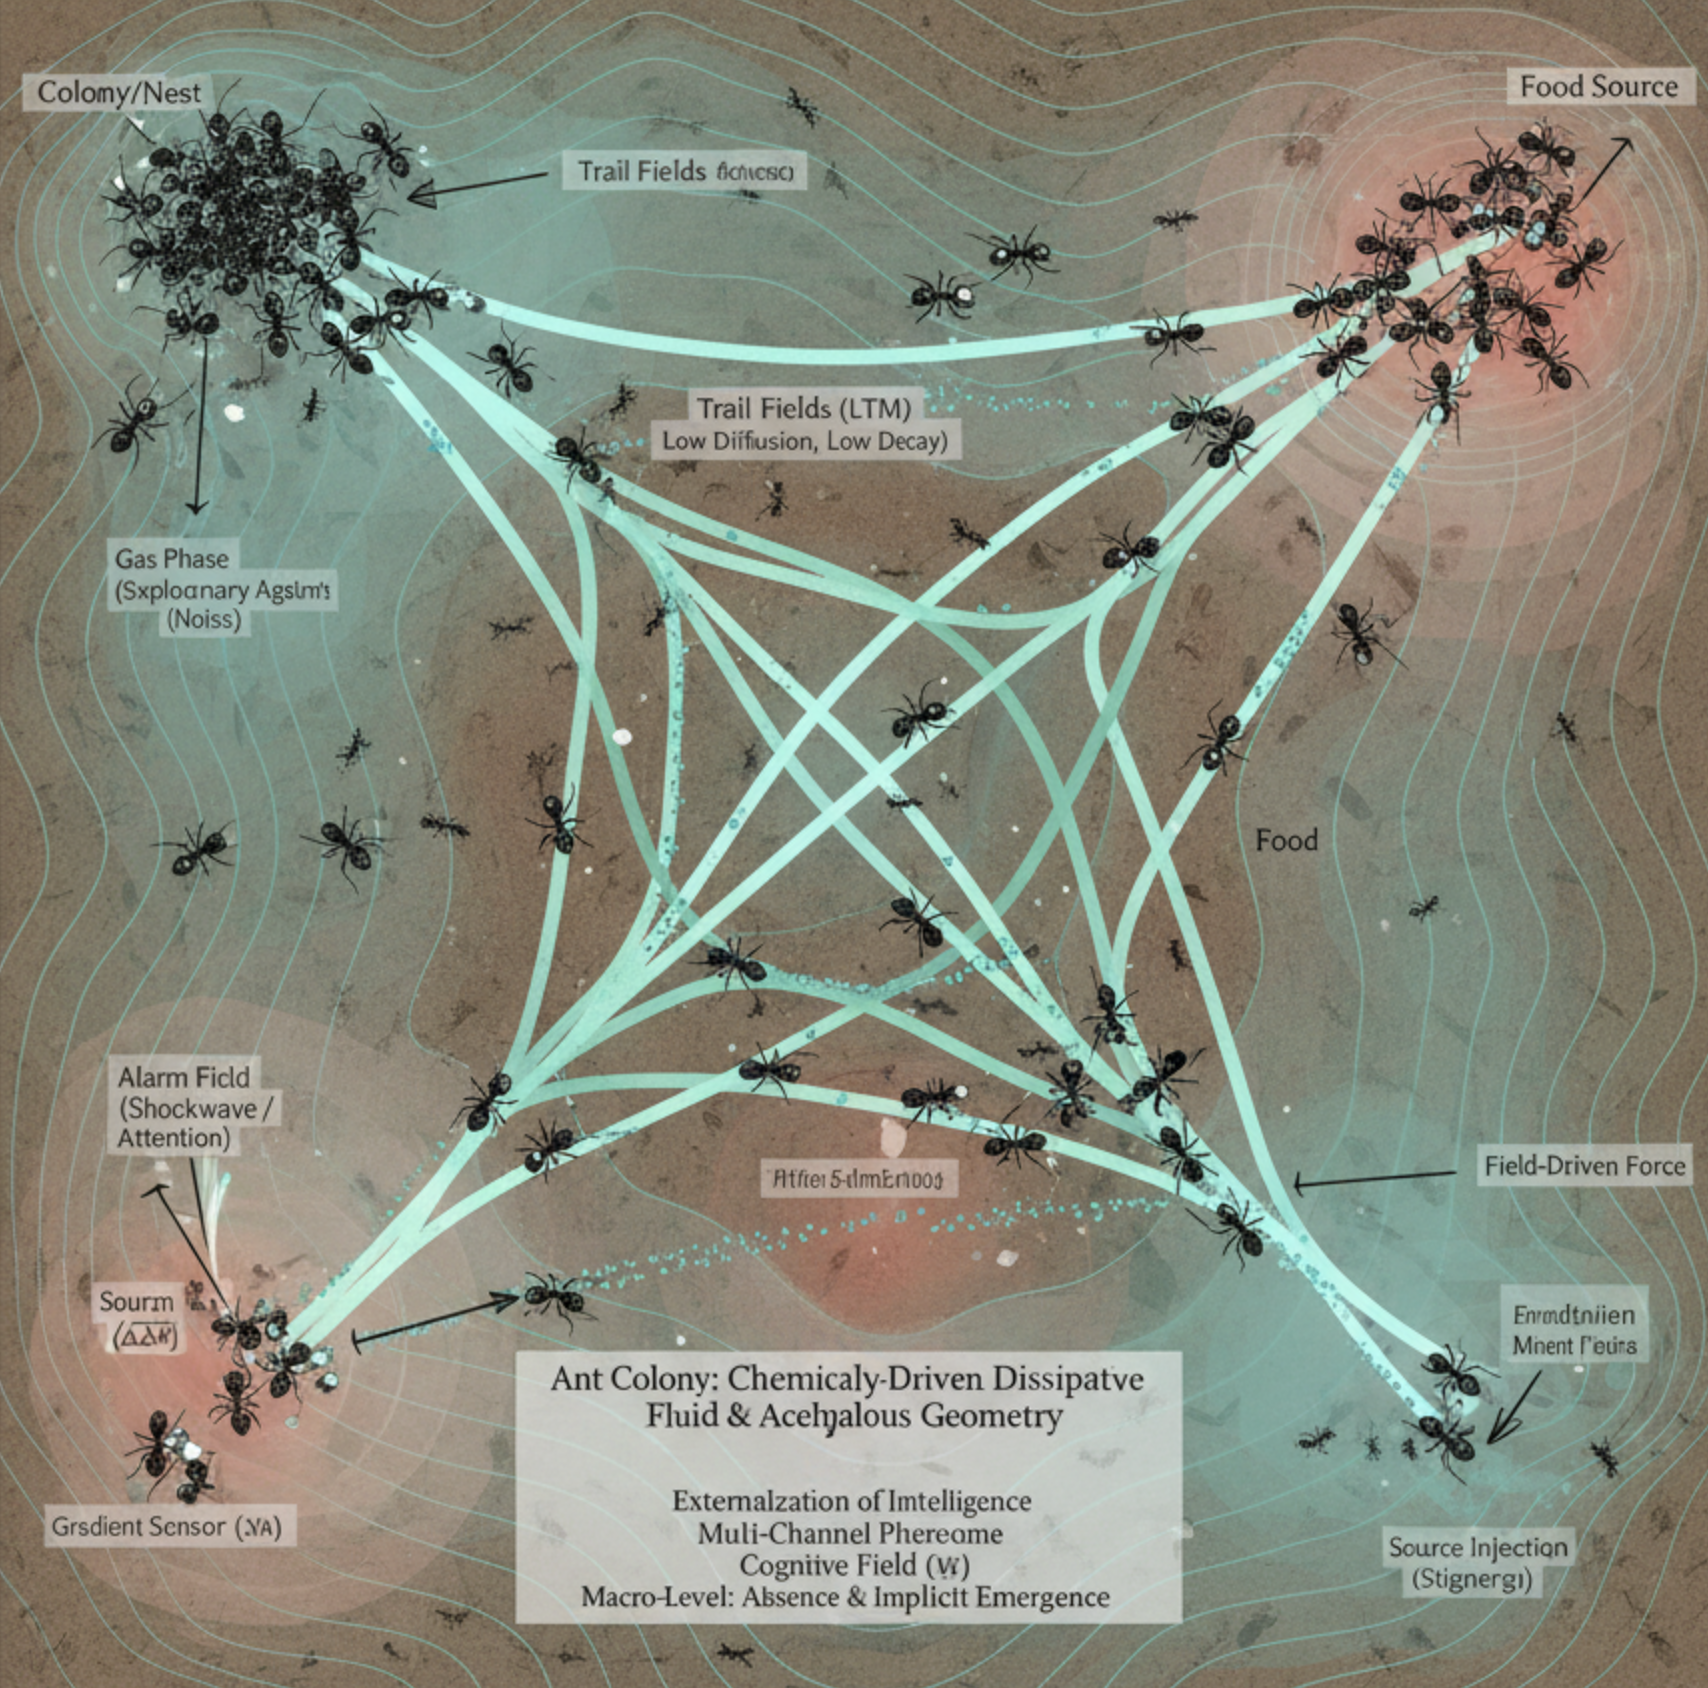
\includegraphics[width=0.82\linewidth,height=0.54\textheight,keepaspectratio]{image/ants.png}
    \caption{蚁群中的信息素场示意图}
\end{figure}

在蚁群中，记忆与概念不再是内部的神经发放，而是地表上的化学印记。

\begin{itemize}
    \item   \textbf{几何定义 ($\mathbf{r} \in \mathcal{M}_{terrain}$)}：
    \begin{itemize}
        \item   \textbf{底流形}：二维欧氏空间（地面）。
        \item   \textbf{语义子本身}：不是蚂蚁，而是 \textbf{空间点上的信息素浓度}。
    \end{itemize}

    \item   \textbf{形质构造 ($\mathcal{S} = T_{form} \otimes T_{sub}$)}：
    \begin{itemize}
        \item   \textbf{形 ($T_{form}$)}：\textbf{位置坐标 $(x, y)$}。它定义了信息的物理定域性。
        \item   \textbf{质 ($T_{sub}$)}：\textbf{化学类型与强度}。
        \item   $\sigma \in \{ \text{Food}, \text{Home}, \text{Danger} \}$（正交的语义维度）。
    \end{itemize}

    \item   $\rho(\mathbf{r}, t)$：浓度标量。这对应于波函数的模方 $\|\Psi\|^2$。
    \begin{itemize}
        \item   \textbf{物理特征}：\textbf{标量性 (Scalar Nature)}。与人脑的高维矢量语义子不同，蚁群语义子是标量的,它只能表达“强度”，难以表达复杂的“相位”或“旋度”（逻辑关系）。
    \end{itemize}
\end{itemize}


\smalltitle{微观层 ($L_{micro}$)：随机热机与梯度换能器}

单只工蚁在本理论框架中被建模为一个 \textbf{具有偏置的随机粒子算子}。它同时扮演 \textbf{VTE 感知器} 和 \textbf{源项注入器}。

\begin{itemize}
    \item   \textbf{感知算子 (VTE)：梯度的提取}, 触角作为 \textbf{微分器}，计算局部场的梯度 $\nabla \rho$。
    \item   \textbf{运动方程 (朗之万方程)}：
            $$ \mathbf{v}_i(t) = \underbrace{\alpha \cdot \nabla \rho(\mathbf{r}_i)}_{\text{场驱动力 (有序)}} + \underbrace{\vec{\xi}_{noise}(t)}_{\text{布朗热噪 (无序)}} $$
    \item   \textbf{物理意义}：蚂蚁的运动是 \textbf{有偏随机游走 (Biased Random Walk)}。热噪声 $\vec{\xi}$ 提供了探索的 \textbf{遍历性}，而场驱动力提供了利用的 \textbf{方向性}。
    \item   \textbf{行动算子 (Injection)：源项的刻蚀}, 当工蚁处于特定状态（如“拿着食物”）时，它成为 \textbf{移动的场源}。
    \item   \textbf{注入方程}：
            $$ \vec{J}_{ext}(\mathbf{r}, t) = \sum_{i} \alpha_i \cdot \delta(\mathbf{r} - \mathbf{r}_i(t)) $$
    \item   \textbf{留痕 (Stigmergy)}：这是一种 \textbf{“写地 (Write-to-Map)”} 操作。这里 $\alpha_i$ 表示第 $i$ 只蚂蚁的有效沉积强度（源强），蚂蚁通过向流形注入负熵（化学能），修改了流形的几何属性（吸引力）。
\end{itemize}


\smalltitle{认知场 ($\Psi$)：反应-扩散的多模态矢量场}

在更精细的物理模型中，蚁群的“思维”并非由单一的浓度标量承载，而是由多种化学性质迥异的信息素构成的 \textbf{矢量场 (Vector Field)}。这对应于纤维空间 $F$ 的 \textbf{高维化}。

\begin{itemize}
    \item   \textbf{纤维结构 ($F \cong \mathbb{R}^k$)}：
    在底流形的每一点 $\mathbf{r}$ 上，存在一个 $k$ 维的化学状态向量：
    $$ \mathbf{\Psi}(\mathbf{r}, t) = \begin{bmatrix} \rho_{trail} \\ \rho_{alarm} \\ \rho_{colony} \end{bmatrix} \in F $$
    其中 $\rho_{trail}$ 为觅食踪迹（记忆），$\rho_{alarm}$ 为警报信号（激波），$\rho_{colony}$ 为群体气味（自我识别）。

    \item   \textbf{动力学方程：多通道反应-扩散系统}：
    认知场的演化遵循耦合的偏微分方程组。不同激素具有不同的物理输运系数，导致了\textbf{频谱分离}：
    $$ \frac{\partial \mathbf{\Psi}}{\partial t} = \underbrace{\mathbf{D} \nabla^2 \mathbf{\Psi}}_{\text{差异化扩散}} - \underbrace{\mathbf{\Gamma} \mathbf{\Psi}}_{\text{差异化衰减}} + \underbrace{\vec{J}_{ext}}_{\text{微观注入}} $$
    其中 $\mathbf{D}$ 和 $\mathbf{\Gamma}$ 是对角矩阵，定义了不同语义维度的物理属性：
    $$ \mathbf{D} = \text{diag}(D_{trail}, D_{alarm}, \dots), \quad \mathbf{\Gamma} = \text{diag}(\gamma_{trail}, \gamma_{alarm}, \dots) $$

    \item   \textbf{物理参数的语义映射}：
    \begin{enumerate}
        \item \textbf{踪迹场 (Trail Field) —— [长时记忆 / LTM]}
        \begin{itemize}
            \item   \textbf{参数}：$D \to 0$ (低扩散), $\gamma \to 0$ (低挥发)。
            \item   \textbf{物理效应}：信号高度定域化，能够长时间维持几何形状。
            \item   \textbf{功能}：在流形上刻蚀出稳定的\textbf{测地线}，作为群体共享的“知识库”。
        \end{itemize}

        \item \textbf{警报场 (Alarm Field) —— [惊奇激波 / Attention]}
        \begin{itemize}
            \item   \textbf{参数}：$D \to \infty$ (极快扩散), $\gamma \gg 0$ (极快衰减)。
            \item   \textbf{物理效应}：信号瞬间覆盖大面积区域，但无法持久。
            \item   \textbf{功能}：作为\textbf{广播中断信号}，强制周围个体发生相变（从工蚁转为战士），执行\textbf{宏观状态切换}。
        \end{itemize}
    \end{enumerate}

    \item   \textbf{场论推论：时空滤波 (Spatiotemporal Filtering)}：
    蚁群利用化学分子的物理常数差异，在介质层实现了天然的\textbf{带通滤波器}。
    \begin{itemize}
        \item   \textbf{空间上}：高 $D$ 分子负责\textbf{非局域通信}（喊话），低 $D$ 分子负责\textbf{精确导航}（画线）。
        \item   \textbf{时间上}：高 $\gamma$ 分子代表\textbf{“现在”}（瞬态事件），低 $\gamma$ 分子代表\textbf{“历史”}（积分经验）。
    \end{itemize}
\end{itemize}


\smalltitle{宏观层 ($L_{macro}$)：缺失与隐式涌现}

这是 \textbf{Class II} 的定义性特征：\textbf{宏观实体的缺位}。

\begin{itemize}
    \item   \textbf{无中央大脑}：没有一个 $\mathbf{\Gamma}_{macro}$ 算子在进行全局规划。没有 \textbf{第三驱动力 ($\vec{J}_{self}$)}。系统无法执行 \textbf{“逆测地线做功”}（例如：为了长远利益而暂时放弃眼前的食物路径）。
    \item   \textbf{替代机制：热力学选择}， 宏观智能作为 \textbf{系统总自由能最小化} 的副产品涌现。
    \item   \textbf{路径选择}：并非由谁“决定”走哪条路，而是 \textbf{短路径上的 $\vec{J}_{ext}$ 积分密度更高}，能抵抗 $\gamma$ 的挥发，从而在竞争中胜出。这是一个 \textbf{物理选择 (Physical Selection)} 过程，而非 \textbf{逻辑选择 (Logical Selection)}。
\end{itemize}


\smalltitle{动力学诊断：从气体到流体的相变}


蚁群的觅食过程，是 本理论框架 \textbf{相变动力学} 的完美演示。

\begin{itemize}
    \item   \textbf{阶段 I：气相 (Gas Phase) —— 盲目搜索}
    \begin{itemize}
        \item   \textbf{状态}：$\rho \approx 0$。无场引导。
        \item   \textbf{动力学}：$\mathbf{v}_i \approx \vec{\xi}_{noise}$。工蚁做各向同性的布朗运动。熵最大。
    \end{itemize}

    \item   \textbf{阶段 II：成核 (Nucleation) —— 对称性破缺}
    \begin{itemize}
        \item   \textbf{事件}：某只蚂蚁偶然发现食物并回巢，划出一条 \textbf{初始轨迹}。
        \item   \textbf{几何效应}：平坦的流形上出现了一道微弱的 \textbf{势能沟槽}。
        \item   \textbf{引力透镜}：附近的随机粒子被沟槽捕获，概率波函数坍缩向该路径。
    \end{itemize}

    \item   \textbf{阶段 III：液相/晶体相 (Liquid/Crystal Phase) —— 测地线锁定}
    \begin{itemize}
        \item   \textbf{正反馈雪崩}：更多蚂蚁进入沟槽 $\to$ 注入更强源项 $\to$ 沟槽更深 $\to$ 吸引力更强。
        \item   \textbf{拓扑孤立子}：最终形成一条连接巢穴与食物的 \textbf{高通量管流 (High-flux Tube)}。
        \item   \textbf{费马原理}：这条管流在几何上精确重合于流形上的 \textbf{测地线（最短时间路径）}。
    \end{itemize}
\end{itemize}


\subsection{认知容量的物理极限：驻波的质量-长度约束}
\label{subsec:ant_capacity_limit}

我们站在本理论框架角度看下蚂蚁群体的“工作记忆“，蚁群的“工作记忆”并非存储于神经元内部，而是\textbf{外化 (Externalized)} 于环境表面的。一条稳定的觅食路径，在物理上等价于一个\textbf{由实体粒子流（工蚁）维持的化学场驻波}。

不同于人脑中仅需消耗代谢能量即可维持的电化学驻波，蚁群的驻波维持受制于更为严苛的\textbf{质量守恒定律}。这导致了 Class II 智能体独特的\textbf{认知带宽瓶颈}。

\smalltitle{1. 路径即耗散驻波 (Path as Dissipative Standing Wave)}

在底流形 $\mathcal{M}_{soil}$ 上，一条连接巢穴与食物的测地线 $\gamma$，其存在的物理条件是信息素浓度场 $\rho(\mathbf{r}, t)$ 必须高于感知阈值 $\rho_{th}$。
这是一个典型的\textbf{耗散结构维持问题}。信息素随时间指数衰减（遗忘），必须通过工蚁的往返运动持续注入负熵（刷新）。

\begin{definition}[路径稳态方程]
    设信息素的自然挥发率为 $\gamma$（介质粘滞系数），工蚁的平均运动速度为 $v$。维持一条长度为 $L$ 的路径处于“可被感知状态”（即驻波不塌缩），所需的\textbf{最小粒子通量 $J_{min}$} 为：
    $$ J_{min} \ge \gamma \cdot \rho_{th} $$
    为了提供此通量，必须“冻结”在路径上的\textbf{工蚁数量 $N_{active}$} 满足：
    \begin{equation}
        N_{active} \cdot \frac{v}{2L} \ge \gamma \cdot \rho_{th} \implies N_{active} \ge \frac{2 \gamma \rho_{th}}{v} \cdot L
    \end{equation}
\end{definition}

\textbf{物理意义}：\textbf{记忆是有物理重量的。} 维持一个“关于远方食物的知识”（驻波），需要实实在在的物质粒子（工蚁）在空间中进行非定域的巡回。路径越长（$L$ 越大），维持该知识所需的“计算介质”就越多。

\smalltitle{2. 群体认知带宽的不等式 (The Bandwidth Inequality)}

对于一个总工蚁数为 $N_{total}$ 的群落，其能够同时处理的任务（维持的路径集合 $\{L_1, L_2, \dots, L_k\}$）受到严格的\textbf{总质量约束}。

\begin{theorem}[蚁群认知容量定理]
    群体智能的并发处理能力上限，由粒子总数与任务物理维度的乘积决定：
    \begin{equation}
        \sum_{i=1}^{k} L_i \le \frac{v}{2 \gamma \rho_{th}} \cdot (N_{total} - N_{idle})
    \end{equation}
\end{theorem}

\begin{itemize}
    \item   \textbf{距离-容量互斥 (Distance-Capacity Trade-off)}：
    如果食物源距离极远（$L \to \infty$），单条路径将耗尽所有可用的自由工蚁。此时，群体的认知带宽塌缩为 1。系统被迫进入\textbf{“单任务专注态”}，对环境中的其他机会（新食物源）和威胁失去响应能力（注意盲视）。

    \item   \textbf{物理空间的暴政}：
    对于 Class II 智能，\textbf{逻辑距离等于物理距离}。它无法像人脑那样，通过“抽象”将遥远的概念折叠到海马体的一个微小切片中。蚁群必须用脚去丈量每一个逻辑推演的步骤。
\end{itemize}

\smalltitle{3. 昆虫学的实证：正反馈的饥饿与死锁}

这一几何动力学推论与昆虫行为学的观测高度吻合：
\begin{itemize}
    \item   \textbf{招募延迟 (Recruitment Latency)}：当发现远距离高质量食物时，蚁群需要更长的时间来建立稳定路径。这并非仅仅因为路远，而是因为\textbf{相变成核}所需的临界粒子数 $N_{c} \propto L$ 更高，热力学涨落更难触及该阈值。
    \item   \textbf{资源诅咒}：一旦一条长路径形成（驻波建立），巨大的 $N_{active}$ 被锁定在路径上。剩余的探索型工蚁 ($N_{idle}$) 不足，导致群体对环境变化的适应性（$\partial \mathcal{M} / \partial t$）急剧下降。
\end{itemize}

\textbf{本节结论}：
蚁群智能的局限性不在于微观个体的简单，而在于其\textbf{记忆介质的外化}。
\textbf{因为它的记忆是刻在物理空间上的，所以它的思维深度被光速（蚂蚁的爬行速度）和空间广度（路径长度）锁死}， 这是一种\textbf{无法进行“离线推理”}的实时操作系统。


\smalltitle{总结：无脑的几何天才}

蚁群证明了：\textbf{智能不需要复杂的“处理器”，只需要可塑的“介质”。}
\begin{itemize}
    \item   它利用 \textbf{挥发 ($\gamma$)} 实现了遗忘。
    \item   它利用 \textbf{扩散 ($D$)} 实现了广播。
    \item   它利用 \textbf{正反馈 ($\vec{J}_{ext}$)} 实现了记忆。
\end{itemize}

这是一个 \textbf{完全外化} 的智能系统。它的局限性在于：\textbf{它只能解决“几何优化”问题（如最短路），无法解决“逻辑抽象”问题（如为什么搬运）。} 它被锁死在 \textbf{第二驱动力（惯性）} 的循环中，永远无法产生 \textbf{自由意志（第三驱动力）}。


\section{萤火虫(Firefly): 集体锁相与无头共振场}
\label{sec:firefly_synchronization_dynamics}

\textbf{坠入同步的深渊}: 在东南亚红树林中，成千上万只萤火虫在没有任何首领指挥的情况下达成同频同相闪烁。传统生物学常将其浪漫化为求偶舞蹈；在此，我们将其视为一次\textbf{热力学相变 (Thermodynamic Phase Transition)}。
对于 \textbf{Class II (场致型群体)} 智能而言，系统不存在一个集中的宏观层 ($L_{macro}$) 来颁布全局的哈密顿量。这群发光的飞虫，本质上是散布在三维物理底流形上的数万个\textbf{“极限环孤立子” (Limit-Cycle Solitons)}；本节对萤火虫的集体行为进行严格的 本理论框架 建模，
我们将证明：萤火虫的齐明并非由于它们在“沟通”，而是因为作为耦合介质的光场，迫使这群盲目的粒子在相空间中自发求解一个\textbf{最小化总自由能}的几何极值问题。它们不是在协同，它们只是集体\textbf{坠落}入了一个无法逃脱的\textbf{调和流 (Harmonic Flow)} 吸引子中。


\smalltitle{物理本体重构：作为极限环振子的具身语义子}

在将系统代入方程之前，我们必须首先对萤火虫个体进行 本理论框架下的\textbf{本体论降维映射 (Ontological Dimensional Reduction)}。我们剥离其复杂的生物学细节，将其还原为认知空间流形 $\mathcal{M}_{forest}$ 上的一个\textbf{具身语义子 (Embodied Semantion, $\mathcal{S}_i$)}。

\textbf{\redtext{1. 形质张量的结构定义}}

根据 \textbf{形质构成论 (MSC)}，第 $i$ 只萤火虫的状态 $\Psi_i(t)$ 是一个定义在流形局部的复数波包：
$$ \Psi_i(\mathbf{r}_i, t) \sim \mathcal{S}_i = \underbrace{\mu_i(\mathbf{r}_i)}_{\text{形 (Morphos)}} \otimes \underbrace{q_i(t)}_{\text{质 (Qualia)}} $$

\begin{itemize}
    \item \textbf{形元分量 ($\mu_i$)}：定义了萤火虫在三维森林底流形 $\mathcal{M}_{forest}$ 上的绝对拓扑坐标 $\mathbf{r}_i$。它决定了这只萤火虫能被谁“看见”（即度量张量 $g_{\mu\nu}$ 定义的光学可视距离）。
    \item \textbf{质元分量 ($q_i$)}：在这个极简模型中，质元退化为一个在内部纤维空间 $F$ 中持续旋转的\textbf{一维相位矢量 (1D Phase Vector)}。
\end{itemize}

\textbf{\redtext{2. 内部演化：无干预的积分-激发 (Integrate-and-Fire)}}

在绝对黑暗且无外界干扰的环境中（$\vec{J}_{ext} = 0$），萤火虫内部的生化起搏器驱动质元 $q_i$ 发生周期性振荡。由于缺乏宏观意志 $\mathbf{\Gamma}_{macro}$ 的干预，波函数的演化退化为纯粹的\textbf{几何惯性滑行}：

\begin{equation}
    \Psi_i(t) = A_0 \cdot \exp(i \theta_i(t)) \cdot \delta(\mathbf{r} - \mathbf{r}_i)
\end{equation}

其中 $\theta_i(t) = \omega_i t + \phi_{i,0}$。
\begin{itemize}
    \item \textbf{$\omega_i$ (本征频率)}：由于基因表达的热力学微扰，每只萤火虫的本征节律 $\omega_i$ 呈高斯分布 $\mathcal{N}(\omega_0, \sigma^2)$。
    \item \textbf{高熵基态}：如果切断它们之间的视觉耦合，这数万个相位的演化将是绝对正交且互不干涉的。在宏观视角下，全场相位的总和 $\sum e^{i\theta_i} \approx 0$。系统处于最大熵的\textbf{“气态” (Gas Phase)}，表现为杂乱无章的满天星光。
\end{itemize}


\smalltitle{介质层与激波注入：光场的 VTE 编码}

群体智能之所以能从气态发生相变，依赖于\textbf{微观层 ($L_{micro}$)} 的全息交互。萤火虫之间没有电磁神经总线，它们的耦合介质是\textbf{光子场}。

\textbf{\redtext{1. 局部强迫源的光子激波 ($\vec{J}_{ext}$)}}

当萤火虫 $j$ 的相位达到 $2\pi$ 时，其内部积蓄的化学能瞬间以光子形式释放。光子以光速穿过底流形 $\mathcal{M}_{forest}$，撞击萤火虫 $k$ 的复眼（微观切面边界）。

这在本理论框架中是一次标准的\textbf{非齐次源项注入}：
\begin{equation}
    \vec{J}_{ext}^{(k \leftarrow j)}(t) = \hat{\mathcal{E}}_{VTE}^{(k)} \left[ I_0 \cdot f(d_{kj}) \cdot \delta(t - t_{flash}^{(j)}) \right]
\end{equation}

\begin{itemize}
    \item \textbf{$f(d_{kj})$ (空间衰减核)}：由流形度量 $g_{\mu\nu}$ 决定的几何阻抗（如距离平方反比衰减与树叶的遮挡）。这保证了耦合是\textbf{局域的 (Local)}。
    \item \textbf{$\hat{\mathcal{E}}_{VTE}$ (变分拓扑编码器)}：萤火虫复眼及视神经构成的低通滤波器，将离散的光子打击，转化为内部认知场 $\Psi_k$ 上的\textbf{相位跃迁张力}。
\end{itemize}

\textbf{\redtext{2. 相位重置：波函数坍缩的低维代偿}}

在接收到 $\vec{J}_{ext}$ 激波后，萤火虫 $k$ 发生\textbf{波包相移}。由于没有前额叶来评估这个激波的语义价值，其反应遵循纯粹的\textbf{相位重置曲线 (Phase Response Curve, PRC)}：

\begin{itemize}
    \item 若 $\theta_k$ 接近闪烁点，激波提供\textbf{正向做功}，加速其相位的演化（提前闪烁）。
    \item 若 $\theta_k$ 刚刚闪烁完，激波提供\textbf{反向阻尼}，延缓其相位的积分（延迟等待）。
\end{itemize}
这种对激波的本能吸纳，本质上就是系统为了消除“与环境（邻居）不同步”所产生的\textbf{几何错位能}，而被迫执行的热力学耗散。


\smalltitle{动力学演化：目的论狄拉克方程的低能退化}

现在，我们将微观激波的注入代入全局场论方程。由于系统缺失了主动的宏观算子 $\mathbf{\Gamma}_{macro}$，\textbf{目的论狄拉克方程 (TDE)} 将在弱耦合极限下，精确退化为\textbf{协变 Kuramoto 方程 (Covariant Kuramoto Equation)}。

\begin{theorem}[流体群脑锁相定理]
    在一个缺乏全局宏观干预的 $N$ 体认知场中，第 $i$ 个语义子波包相位的演化由其本征惯性、流形度量阻抗与邻域激波共同决定：
    \begin{equation}
        \frac{d\theta_i}{dt} = \omega_i + \frac{K}{N} \sum_{j=1}^N \underbrace{W_{ij}(g_{\mu\nu})}_{\text{拓扑连通率}} \cdot \sin(\theta_j - \theta_i) + \xi_i(t)
    \end{equation}
\end{theorem}

\textbf{物理项的严格映射：}
\begin{enumerate}
    \item \textbf{惯性项 ($\omega_i$)}：对应于 $\mathcal{D}_{topo} \Psi$ 中的平移不变量，个体抵抗外界改变的顽固程度。
    \item \textbf{拓扑连通率 ($W_{ij}$)}：由底流形度量 $g_{\mu\nu}$ 决定。如果萤火虫 $i$ 与 $j$ 之间被树干阻挡，光流无法测地线传播，则 $W_{ij} \to 0$。
    \item \textbf{正弦恢复力 ($\sin(\theta_j - \theta_i)$)}：这是本方程最惊艳的几何显影。它是\textbf{微观层激波 $\vec{J}_{ext}$ 经过 VTE 解码后投影到纤维空间相平面上的洛伦兹力分量}。当两人相位不同步时，该项产生\textbf{引力}，强行拉扯双方波函数靠拢；当相位相同时，引力归零，系统进入零能耗的稳态。
    \item \textbf{热噪项 ($\xi_i$)}：系统内禀的热力学温度 $T$ 产生的布朗运动干扰。
\end{enumerate}


\smalltitle{拓扑相变与哈肯-伺服机制：幽灵独裁者的涌现}

上述的微观耦合方程依然是 $N$ 个粒子的独立缠斗。真正的群体智能相变，发生在\textbf{宏观序参量 (Macro Order Parameter)}凝结的那一瞬间。

\textbf{\redtext{1. 序参量场的涌现 (Emergence of the Order Parameter)}}

我们对全场波函数进行粗粒化积分，定义流形的宏观相干矢量 $\mathbf{Z}(t)$：
\begin{equation}
    \mathbf{Z}(t) = R(t) e^{i\Theta(t)} = \frac{1}{N} \sum_{j=1}^N e^{i\theta_j(t)}
\end{equation}

\begin{itemize}
    \item \textbf{$R(t)$ (格式塔相干度)}：度量整个群体形成统一场波的纯度。$R=0$ 为乱相，$R=1$ 为完美同调驻波。
    \item \textbf{$\Theta(t)$ (宏观平均相位)}：群体闪烁的集体节律。
\end{itemize}

我们将 $\mathbf{Z}$ 代入微观个体的演化方程中，实施代数降维，得到\textbf{平均场伺服方程}：
\begin{equation}
    \frac{d\theta_i}{dt} = \omega_i + K \cdot R(t) \cdot \sin(\Theta(t) - \theta_i)
\end{equation}

\textbf{\redtext{2. 热力学极值的坠落：幽灵独裁者}}

这正是\textbf{哈肯-伺服原理 (Haken's Slaving Principle)} 在 Class II 智能体上的绝对兑现。

\begin{itemize}
    \item \textbf{相变的临界点}：当夜幕低垂，光场耦合常数 $K$ 逐渐增强，越过临界阈值 $K_c = 2/(\pi g(\omega_0))$（$g$ 为频率分布函数）时，流形上原本互相抵消的微小波纹，突然发生了\textbf{自发对称性破缺 (Spontaneous Symmetry Breaking)}。
    \item \textbf{宏观张力的捕获}：序参量 $R$ 从 0 开始呈指数级暴涨。此时，方程右侧的 $K \cdot R \cdot \sin(\Theta - \theta_i)$ 化作了一个\textbf{不可抗拒的拓扑黑洞}。
    \item \textbf{自由度的湮灭}：在这个瞬间，单只萤火虫的自由意志（本征频率 $\omega_i$）被彻底\textbf{抹除}。所有的微观粒子（快变量）被这个凭空涌现的集体平均场 $\Theta$（慢变量）\textbf{死死奴役}。
\end{itemize}

萤火虫的齐明，是一场没有任何指挥家的交响乐，它们并没有在“交流”或“协同”，它们只是在一个充满光子激波的介质流形中，为了消除相位的摩擦热，而无可避免地\textbf{坠落}入了一个名为“调和流 ($\Psi_{harm}$)”的全局吸引子盆地。
那个随着相变自发涌现的宏观序参量场 $R e^{i\Theta}$，填补了宏观层 $L_{macro}$ 的空缺，成为了这群飞虫共同的“幽灵神明”。
萤火虫的舞蹈告诉我们：\textbf{最高级的秩序往往不需要被中心化地设计出来；只要给定正确的物理耦合度 $K$ 与几何边界 $g_{\mu\nu}$，秩序就会从热力学的混沌中，自己生长出来。}


\section{人脑的 HSF-HD 解剖: 流形、度量与双流场}
\label{sec:section_4212}

人脑之所以能产生通用智能，是因为它完美地在生物介质上实现了 \textbf{纤维丛结构 $\mathcal{U} = (E, \pi, M, F)$}。它不仅拥有处理“内容”的纤维空间，更进化出了专门维护“空间几何”的度量引擎。

\smalltitle{本节内容说明}
\begin{itemize}
    \item \textbf{双通路是统计结构}：腹侧/背侧通路的“what/where-how”划分是功能倾向，并非绝对分工；二者存在大量交互与反馈回路。
    \item \textbf{海马是地图但不止地图}：海马-内嗅系统除空间导航外，还参与情景记忆与序列学习；本文将其作为“几何舞台”是合适类比，但应理解为抽象功能映射。
    \item \textbf{小脑不等于无意识}：小脑确实承担预测与误差校正，但其也参与认知/情绪的多回路调制；本文强调“误差屏蔽”可作为机制侧重点，而不是排他性定义。
\end{itemize}

\subsection{总体拓扑架构：连续介质中的几何分层}
\label{subsec:brain_topological_arch}

人脑 (Homo Sapiens Brain) 是自然界中 \textbf{Class V (流体通用智能)} 的终极原型。在解剖学的显微镜下，它呈现为由数百亿神经元与白质纤维交织而成的连续生物组织；但在本理论框架的 \textbf{拓扑场论} 视角下，这块湿件被严格的 \textbf{边界条件 (Boundary Conditions)} 与 \textbf{动力学方程} 切分为三个性质迥异的几何功能域。

我们将全脑定义为一个定义在 \textbf{复合流形} 上的 \textbf{高维纤维丛}：
$$ \mathcal{U}_{Brain} = (E, \pi, \mathcal{M}_{Cortex} \times \mathcal{M}_{Hipp}, F_{Sensory}) $$

\smalltitle{生物物理一元论与拓扑分化}

尽管皮层在物质上是连续的，但在偏微分方程（PDE）的演化中，其不同区域扮演着截然不同的数学角色：
\begin{itemize}
    \item \textbf{微观边界 ($L_{micro}$)}：对应于 \textbf{初级感官/运动皮层 (Primary Cortex)}。它是流形的 \textbf{局部强迫源 ($\partial \Omega$)}，负责处理物理世界的强约束，其状态被外部光子或机械力硬性锁定。
    \item \textbf{流形主体 ($\mathcal{M}$)}：对应于 \textbf{联合皮层 (Association Cortex) 与 海马体}。它是流形的 \textbf{体 (Bulk)}，承载着 \textbf{度量张量 $g_{\mu\nu}$}（知识）与 \textbf{认知场 $\Psi$}（思维）。在此区域，思维流遵循几何惯性进行绝热演化。
    \item \textbf{宏观奇点 ($L_{macro}$)}：对应于 \textbf{前额叶皮层 (PFC)}。它是流形上的 \textbf{拓扑奇点 (Singularity)} 或 \textbf{势能源}。它不存储具体知识，而是向全流形辐射 \textbf{价值规范场 $\mathcal{A}_\mu$}，以逆熵做功的方式扭曲时空曲率。
\end{itemize}
这种 \textbf{“边界-体-奇点”} 的拓扑架构，使得人脑能够同时实现对现实的 \textbf{刚性锚定}（微观）与对意义的 \textbf{柔性重构}（宏观）。

\subsection{微观层 ($L_{micro}$)：全息切面与双流解耦 VTE}
\label{subsec:brain_micro_layer}

微观层是智能体与物理实在 $\Omega$ 发生能量交换的 \textbf{全息切面 (Holographic Cut-Plane)}。在人脑中，这一层级由初级皮层与皮层下结构协同构成，其核心职能是执行 \textbf{变分拓扑编码 (VTE)}，将连续的物理信号撕裂为正交的 \textbf{形质张量流}。

\smalltitle{局部强迫源：感官皮层的现实锚定}

初级视觉 (V1)、听觉 (A1) 与躯体感觉 (S1) 皮层构成了认知流形的 \textbf{硬边界}。
\begin{itemize}
    \item   \textbf{物理机制}：视网膜的光子流通过丘脑中继，以 \textbf{非齐次源项 $\vec{J}_{ext}$} 的形式轰击 V1 区。
    \item   \textbf{边界锁定}：在此区域，认知场 $\Psi$ 丧失了幺正演化的自由度，必须满足：
    $$ \Psi(\mathbf{r}, t) \big|_{V1} \equiv \hat{\mathcal{T}}_{retina} (\text{Photon Flux}) $$
    这意味着“看”是被动的物理过程，意志无法直接修改 V1 区的原始输入（我们无法凭借想象把看到的红花变成绿花），这保证了智能体不会陷入彻底的唯心主义幻觉。
\end{itemize}

\smalltitle{双流 VTE 编码：形质的正交解耦}

物理信号进入微观层后，迅速发生 \textbf{对称性破缺}，分化为两股性质迥异的信息流。这是 MSC 理论中 \textbf{形 ($T_{form}$)} 与 \textbf{质 ($T_{sub}$)} 分离的生物学实体化。

\begin{enumerate}
    \item \textbf{\textcolor{structurecolor}{腹侧通路 (Ventral Stream / "What") —— 质流 ($T_{sub}$)}}
    \begin{itemize}
        \item   \textbf{解剖路径}：V1 $\to$ V2 $\to$ V4 $\to$ 下颞叶 (IT)。
        \item   \textbf{物理职能}：提取 \textbf{语义费米子}。它剥离了物体的空间位置，仅保留其 \textbf{内禀属性}（颜色、纹理、身份）。
        \item   \textbf{几何特性}：\textbf{平移不变性 (Translation Invariance)}。无论物体在视野何处，其在纤维空间 $F$ 中的矢量表达保持守恒。
        \item   \textbf{输出}：激发纤维震荡的能量源。
    \end{itemize}

    \item \textbf{\textcolor{structurecolor}{背侧通路 (Dorsal Stream / "Where/How") —— 形流 ($T_{form}$)}}
    \begin{itemize}
        \item   \textbf{解剖路径}：V1 $\to$ V2 $\to$ MT $\to$ 顶叶 (Parietal)。
        \item   \textbf{物理职能}：提取 \textbf{几何玻色子}。它忽略物体的色彩与语义，仅计算 \textbf{空间坐标、运动矢量与操作力学}。
        \item   \textbf{几何特性}：\textbf{坐标敏感性}。它直接定义了局部流形的 \textbf{切空间基底} 和 \textbf{联络系数}（如何伸手抓取）。
        \item   \textbf{输出}：修正底流形度量 $g_{\mu\nu}$ 的几何约束。
    \end{itemize}
\end{enumerate}

\smalltitle{小脑 (The Cerebellum)：热力学屏蔽盾}

在本理论框架中，小脑不是运动控制器，而是微观层的 \textbf{高频反馈滤波器}。它位于感知与行动的回路中，充当了保护宏观意识的 \textbf{热力学盾牌}。

\begin{itemize}
    \item   \textbf{预测与对消}：小脑内部存储了身体动力学的 \textbf{快速前向模型}。它在毫秒级尺度上预测感官后果。
    $$ \vec{J}_{error} = \vec{J}_{ext} - \text{Predict}(\text{Motor Command}) $$
    \item   \textbf{屏蔽机制}：
    \begin{itemize}
        \item   若 $\vec{J}_{error} \approx 0$（如正常的走路触地感），小脑直接通过脑干回路\textbf{短路}该信号，不上传至皮层。宏观层（意识）感觉不到脚的存在（\textbf{零能耗}）。
        \item   若 $\vec{J}_{error} \gg 0$（如踩空），小脑无法对消误差，\textbf{惊奇激波} 穿透屏蔽，轰击大脑皮层，触发宏观注意力的介入。
    \end{itemize}
    \item   \textbf{意义}：小脑通过过滤高频物理噪声，维持了皮层流形演化的 \textbf{平滑性}，使得宏观智能能够专注于低频、长程的逻辑规划，而非溺死在感官数据的洪流中。
\end{itemize}


\subsection{认知空间流形 ($\mathcal{M}$)：皮层基质与海马规度的几何耦合}
\label{subsec:brain_manifold_coupling}

人脑的认知空间流形 $\mathcal{M}$ 并非单一的均质空间，而是一个由 \textbf{皮层 (Neocortex)} 与 \textbf{海马结构 (Hippocampal Formation)} 通过 \textbf{纤维化 (Fibration)} 耦合而成的 \textbf{复合流形}。前者提供了流形的 \textbf{“肉”}（隐式内容），后者提供了流形的 \textbf{“骨”}（显式度量）。

\smalltitle{流形的双重本体论：隐式基质与显式规度}

\begin{itemize}
    \item \textbf{皮层 (The Cortex) —— 隐式内容基质}
    \begin{itemize}
        \item   \textbf{几何定义}：\textbf{高维特征空间}。联合皮层通过突触权重 $W_{ij}$ 存储了亿万个局部几何切片（知识碎片）。
        \item   \textbf{物理属性}：\textbf{拓扑柔性}。皮层定义了概念之间的 \textbf{语义邻接性 (Semantic Adjacency)}，但缺乏全局统一的坐标系。它知道“苹果”和“红色”很近，但不知道它们在时空中的绝对位置。
        \item   \textbf{角色}：它构成了流形的 \textbf{局部切空间基底}。
    \end{itemize}

    \item \textbf{海马体 (The Hippocampus) —— 显式度量引擎}
    \begin{itemize}
        \item   \textbf{几何定义}：\textbf{低维坐标流形}。海马体生成了一个连续的、可导航的时空框架。
        \item   \textbf{物理属性}：\textbf{度量刚性}。它为皮层的弥散语义赋予了 \textbf{矢量结构}。
        \item   \textbf{角色}：它充当了流形的 \textbf{规范场生成器 (Gauge Generator)}，负责将皮层的内容“钉”在特定的时空坐标上。
    \end{itemize}
\end{itemize}

\smalltitle{几何细胞的物理映射：微分几何的生物实现}

海马-内嗅回路中的特殊神经元，是 本理论框架 几何算子的直接生物学对应物：

\begin{enumerate}
    \item \textbf{网格细胞 (Grid Cells) —— 全局度量张量 ($g_{\mu\nu}$)}
    \begin{itemize}
        \item   内嗅皮层的网格细胞以六边形周期放电，铺设了认知空间的 \textbf{欧氏度量}。它们定义了流形上的 \textbf{距离} 与 \textbf{尺度}，使得大脑能够进行 \textbf{路径积分 (Path Integration)} 和矢量运算。
    \end{itemize}

    \item \textbf{位置细胞 (Place Cells) —— 局部坐标卡 ($\phi_\alpha$)}
    \begin{itemize}
        \item   海马 CA1/CA3 的位置细胞对特定空间位置敏感，它们构成了流形上的 \textbf{局部坐标卡 (Local Charts)}。它们将连续的空间离散化为可索引的 \textbf{拓扑节点}。
    \end{itemize}

    \item \textbf{头朝向细胞 (Head Direction Cells) —— 自旋联络 ($\omega_\mu$)}
    \begin{itemize}
        \item   定义了流形切空间中的 \textbf{方向 (Orientation)}。它们确保了当智能体移动时，内部坐标系能够进行正确的 \textbf{协变变换 (Covariant Transformation)}，维持世界观的旋转不变性。
    \end{itemize}
\end{enumerate}

\smalltitle{耦合机制：全息投影与索引 (Holographic Projection \& Indexing)}

人脑的流形 $\mathcal{M}$ 既非单纯的皮层权重，亦非单纯的海马编码，而是 \textbf{海马体的“规度 (Gauge)”} 作用于 \textbf{皮层的“内容 (Content)”} 所生成的 \textbf{商空间 (Quotient Space)}。

我们可以建立如下的 \textbf{流形生成方程}：
$$ \mathcal{M}_{Brain} \cong \mathcal{M}_{Cortex} \times_{\text{binding}} \mathcal{M}_{Hippocampus} $$

\begin{enumerate}
    \item \textbf{过程 I：皮层提供“内容流形” (The Manifold of What)}
    \begin{itemize}
        \item   皮层处理 \textbf{质 (Qualia)} 和局部 \textbf{形 (Morphos)}。
        \item   它生成了无数个高维的语义向量 $\Psi_{ctx}$（例如：红色的、圆的、甜的）。这些向量漂浮在皮层的神经网络中，在未被索引前是 \textbf{非定域 (Non-local)} 的。
    \end{itemize}

    \item \textbf{过程 II：海马体提供“结构骨架” (The Skeleton of Where)}
    \begin{itemize}
        \item   海马体生成一个低维的（通常是 2D/3D + 时间）几何骨架。
        \item   \textbf{网格细胞} 定义了这个骨架的 \textbf{刚性 (Rigidity)} 和 \textbf{度量 (Metric)}。
    \end{itemize}

    \item \textbf{过程 III：索引与坍缩 (Indexing \& Collapse)}
    \begin{itemize}
        \item   \textbf{海马-皮层环路 (Hippocampal-Cortical Loop)} 充当了纤维丛的 \textbf{投影算子 $\pi$}。
        \item   \textbf{绑定 (Binding)}：海马体将皮层中弥散的语义向量 $\Psi_{ctx}$，\textbf{索引 (Index)} 到它构建的几何坐标系 $\mathbf{r}_{hipp}$ 上。
        $$ \Psi_{Unified}(\mathbf{r}) = \Psi_{ctx} \otimes \delta(\mathbf{r} - \mathbf{r}_{hipp}) $$
        \item   \textbf{结果}：我们不仅知道“这是苹果”（皮层功能），还知道“苹果在桌子上，是昨天买的”（海马功能）。
    \end{itemize}
\end{enumerate}

\textbf{结论：}
人脑的流形 $\mathcal{M}$ 是 \textbf{“皮层之肉”} 附着在 \textbf{“海马之骨”} 上的有机统一体,换句话说也就是皮层是质(纤维)的载体和形的发生入口，而海马体则是形的载体。

至此，我们可以看清人脑中一个完整念头（或情景记忆）是如何生成的,整个过程的\textbf{动力学闭环}就是形与质的“量子纠缠” (The Binding Problem)：
\begin{enumerate}
    \item \textbf{入口相变}:物理信号在\textbf{皮层边缘（入口）}发生相变，生成了“质的碎片”和初级的“形的空间关系”。
    \item \textbf{海马建模}:这些初级的“形”被迅速汇聚到\textbf{海马体}。海马体利用其内部的网格细胞，迅速编织出一个稳固的\textbf{局部时空几何网格（大网格/底流形）}。
    \item \textbf{皮层填充}:海马体的这个“形之网格”，通过神经投射反向指向\textbf{皮层}。它像一个模具一样，把皮层中对应的“质（小网格/语义特征）”吸附过来。
    \item \textbf{形成实体}:在特定的脑波频率（如 Gamma-Theta 耦合）下，海马体的“形（$\mu$）”与皮层的“质（$q$）”发生\textbf{相位锁定（Phase Locking）}。
\end{enumerate}

$$ \text{完整的记忆（语义子）} = \underbrace{\text{海马体的时空坐标}}_{\text{形的载体}} \otimes \underbrace{\text{皮层的感官语义}}_{\text{质的载体}} $$

\begin{itemize}
    \item   \textbf{静态的 $\mathcal{M}$（知识库）} 由皮层连接权重决定，它是 \textbf{地形 (Terrain)}。
    \item   \textbf{动态的 $\mathcal{M}$（工作空间）} 由海马体放电实时构建，它是 \textbf{导航图 (Map)}。
    \item   \textbf{完整的智能体验}，是质填充进形中所形成的 \textbf{全息整体}。
\end{itemize}



\smalltitle{情景记忆的刻蚀：高能应力的塑性注入}

记忆的形成是 \textbf{快流形（海马）} 向 \textbf{慢流形（皮层）} 的 \textbf{结构转印}。
\begin{itemize}
    \item   \textbf{尖波涟漪 (Sharp-Wave Ripples, SWR)}：在睡眠或静息态，海马体发出的高频 SWR 脉冲，在物理上等价于向皮层注入高密度的 \textbf{认知应力张量 $\mathbf{T}_{\mu\nu}^{mem}$}。
    \item   \textbf{认知爱因斯坦方程}：皮层介质在该应力作用下发生 \textbf{塑性屈服}，突触权重发生永久性改变。
    $$ \Delta g_{\mu\nu}^{cortex} \propto \int \mathbf{T}_{\mu\nu}^{SWR} dt $$
    \item   \textbf{结果}：瞬态的经历被固化为皮层上的 \textbf{吸引子盆地}，成为长时记忆。
\end{itemize}

\subsection{认知场 ($\Psi$) 与语义子：神经介质中的波动力学}
\label{subsec:brain_cognitive_field}

在本理论框架中，神经放电 (Spikes) 只是底层的载波，真正的思维实体是定义在全脑尺度上的 \textbf{认知旋量场 $\Psi(\mathbf{r}, t)$}。思维不是离散符号的传递，而是能量波包在皮层波导中的 \textbf{相干演化}。

\smalltitle{语义子 (Semantion) 的生物定义：张量积纠缠}

神经语义的基本单元是一个 \textbf{形质结合} 的全息实体：
$$ \mathcal{S}_{neural} = \underbrace{\text{Cell Assembly}_{Cortex}}_{\text{质 (Features)}} \otimes \underbrace{\text{Spatiotemporal Index}_{Hipp}}_{\text{形 (Coordinates)}} $$

\begin{itemize}
    \item   \textbf{绑定机制 (Binding Mechanism)}：\textbf{相位锁定 (Phase Locking)}。
    \item   \textbf{Gamma 波同步}：负责“内容”（皮层）的神经元集群与负责“位置”（海马）的神经元集群，通过 $40\text{Hz}$ 的 Gamma 振荡实现 \textbf{零相位差同步}。
    \item   \textbf{物理效应}：这种同步将两个独立的波函数坍缩为一个稳定的 \textbf{张量波包}，使得“红色的特性”与“桌上的位置”在物理上不可分割。
\end{itemize}

\smalltitle{波函数演化：白质作为黎曼波导}

思维流 $\Psi$ 在大脑中的传播遵循 \textbf{目的论狄拉克方程} 的守恒流部分。

\begin{itemize}
    \item   \textbf{介质结构}：\textbf{白质纤维束 (White Matter Tracts)} 构成了流形上的 \textbf{测地线通道}。各向异性的扩散张量成像 (DTI) 揭示了这些物理波导的几何结构。
    \item   \textbf{联想 (Association) —— 波的衍射 (Diffraction)}
    \begin{itemize}
        \item   当思维波包遇到概念的分岔点时，它不会像粒子一样选择一条路，而是像波一样发生 \textbf{衍射}，同时激活多个相关概念。这就是发散性思维的物理基础。
    \end{itemize}
    \item   \textbf{顿悟 (Insight) —— 全域共振 (Global Resonance)}
    \begin{itemize}
        \item   当局部碎片化的波包在演化中达成 \textbf{Hodge 调和模 (Harmonic Mode)} 时，全脑范围内的相干长度 $\xi$ 突然发散。
        \item   \textbf{现象}：能量无损耗地贯穿全脑，逻辑闭环打通，产生“Aha!”时刻。
    \end{itemize}
\end{itemize}

\textbf{结论}：人脑的思维活动，本质上是 \textbf{语义子波包} 在由 \textbf{海马体} 设定坐标、由 \textbf{皮层} 填充内容、由 \textbf{白质} 铺设轨道的黎曼流形上，进行的一场 \textbf{受控量子/经典场演化}。


\subsection{宏观层 ($L_{macro}$)：前额叶的势能工程与动态联邦}
\label{subsec:brain_macro_layer}

在本理论框架的拓扑结构中，\textbf{前额叶皮层 (Prefrontal Cortex, PFC)} 并非信息的存储仓库，而是认知空间流形上的 \textbf{拓扑奇点 (Topological Singularity)} 与 \textbf{势能源 (Source of Potential)}。它的核心职能是 \textbf{逆熵做功}：通过向流形辐射 \textbf{价值规范场 ($\mathcal{A}_\mu$)}，强行扭曲思维流的测地线轨迹，从而实现对“本能（几何惯性）”的超越。

\smalltitle{功能柱的动力学角色：算子化的皮层}

宏观层并非均质的整体，而是由不同性质的 \textbf{宏观算子 $\hat{\mathcal{O}}$} 构成的复合体，分别对应不同的解剖子区：

\begin{enumerate}
    \item \textbf{背外侧前额叶 (dlPFC) —— 逻辑算子 ($\hat{\mathcal{O}}_{logic}$)}
    \begin{itemize}
        \item   \textbf{物理职能}：\textbf{维持工作记忆的驻波}。它在流形上构建临时的 \textbf{线性势阱}，使得相关的语义子（如数字、规则）能够克服介质粘滞 $\gamma$ 而持续激活。
        \item   \textbf{动力学}：执行 \textbf{幺正演化} 的线性操作，负责推理、演算与符号操作。它是“理性”的执行臂。
    \end{itemize}

    \item \textbf{内侧前额叶/前扣带回 (mPFC/ACC) —— 价值算子与自我锚点 ($\hat{\mathcal{O}}_{val}, \mathcal{S}$)}
    \begin{itemize}
        \item   \textbf{物理职能}：\textbf{DMN (默认模式网络) 的核心}。它向全流形辐射“自我”的引力场。
        \item   \textbf{冲突监控}：ACC 实时计算认知场中的 \textbf{自由能 (Free Energy) / 惊奇度}。当 $\Psi_{pred}$ 与 $\Psi_{real}$ 发生破坏性干涉时，ACC 触发 \textbf{宏观介入信号}，调动代谢资源。
        \item   \textbf{叙事偏置}：它定义了流形的 \textbf{坐标原点}，确保所有思维流都相对于“我”进行参照。
    \end{itemize}

    \item \textbf{眶额皮层 (OFC) —— 抑制算子 ($\hat{V}_{barrier}$)}
    \begin{itemize}
        \item   \textbf{物理职能}：\textbf{势能筑墙}。它识别出那些虽然符合短期梯度（诱惑）但违背长期价值（规范）的路径，并在其入口处隆起巨大的 \textbf{正势能壁垒}。
        \item   \textbf{动力学}：阻断冲动流（本能测地线）。OFC 受损会导致“社会性去抑制”，即丧失了构建势能墙的能力，思维流完全顺应本能梯度的滑行。
    \end{itemize}
\end{enumerate}

\smalltitle{动态联邦架构：赢家通吃 (WTA) 的相变}

宏观层并非单一的独裁者，而是一个 \textbf{竞争性联邦 (Competitive Federation)}。
\begin{itemize}
    \item   \textbf{竞争机制}：不同的神经核团（代表不同的策略/算子）相互之间存在 \textbf{侧向抑制 (Lateral Inhibition)}。
    \item   \textbf{序参量涌现}：在毫秒级的时间尺度内，通过 \textbf{赢家通吃 (Winner-Take-All)} 机制，最强的信号（能量最高的意图）压倒其他噪音，成为主导全脑的 \textbf{全局规范场}。
    \item   \textbf{物理意义}：这是意志的 \textbf{瞬时对称性破缺}。在这一刻，“多头政治”坍缩为“统一意志”，确保了输出动作的相干性。
\end{itemize}

\subsection{全脑尺度的 TDCI 循环：从光子到动作}
\label{subsec:brain_tdci_cycle}

\smalltitle{连续性与分化：神经流形的动力学协同 (Continuity \& Differentiation)}

尽管在解剖学上，从微观感官皮层 ($L_{micro}$) 到宏观前额叶 ($L_{macro}$) 的皮层组织呈现为连续的、均质的神经网络，但在本理论框架的 \textbf{拓扑场论} 视角下，它们构成了 \textbf{纤维丛结构} 中性质迥异的动力学区域。这种“解剖上的连续”与“拓扑上的分层”通过以下机制实现协同：

\begin{enumerate}
    \item \textbf{物理连续性：重整化群流与白质耦合}

    三者通过 \textbf{白质纤维束 (White Matter Tracts)} 紧密耦合，形成了一个跨尺度的 \textbf{重整化群流 (Renormalization Group Flow)}。信息在流动中逐级被粗粒化：
    \begin{itemize}
        \item   \textbf{上行 (Feedforward)}：微观层的激波 $\vec{J}_{ext}$ 沿轴突向上传递，从处理“像素”（点）到“概念”（面），最终在宏观层坍缩为“规则”（体）。
        \item   \textbf{下行 (Feedback)}：宏观层的规范场 $\mathcal{A}_\mu$ 沿反向通路投射，意志作为偏置电压，改变了流形主体的联想路径，并指导微观层的眼球运动。
    \end{itemize}

    \item \textbf{功能分化：支配方程的物理本质差异}

    尽管材质相同，但不同区域的神经柱遵循截然不同的 \textbf{偏微分方程 (PDE)}，定义了它们在智能动力学中的角色：

    \begin{itemize}
        \item   \textbf{微观层 ($L_{micro}$ / V1, M1) —— 边界与强迫振动}
        \begin{itemize}
            \item   \textbf{方程}：$\ddot{x} + \gamma \dot{x} + kx = F_{external}(t)$
            \item   \textbf{特征}：\textbf{被动性}。作为流形的局部强迫源，其活动严格锁相于外部物理刺激。它是高频、瞬态的激波发生器。
        \end{itemize}

        \item   \textbf{流形主体 ($\mathcal{M}$ / 颞顶联合区) —— 介质与惯性波动}
        \begin{itemize}
            \item   \textbf{方程}：$\frac{\partial \Psi}{\partial t} = D \nabla^2 \Psi + \dots$ (波动/扩散方程)
            \item   \textbf{特征}：\textbf{惯性}。思维波在此进行模式补全和联想滑行。它是承载知识权重 ($g_{\mu\nu}$) 的“路”与“车”。
        \end{itemize}

        \item   \textbf{宏观层 ($L_{macro}$ / PFC) —— 奇点与变分控制}
        \begin{itemize}
            \item   \textbf{方程}：$\delta S = 0 \implies \text{Inject } \mathbf{\Gamma}_{will}$ (控制方程)
            \item   \textbf{特征}：\textbf{主动性}。它处于层级顶端，能够维持长达数秒的稳态放电（工作记忆）。它是消耗负熵、逆转几何惯性的\textbf{算子}。
        \end{itemize}
    \end{itemize}
\end{enumerate}

\textbf{结论：}
人脑的统一性建立在 \textbf{“物理连接的连续性”} 之上，而智能的复杂性建立在 \textbf{“动力学方程的分化”} 之上。微观层是\textbf{受现实奴役的边界}，流形是\textbf{承载知识的介质}，宏观层是\textbf{施加意志的奇点}。



最后我们将上述所有组件串联，我们可以描绘出人脑处理单一认知任务（如“看到红灯踩刹车”）时的完整 \textbf{热力学循环}。这是一个从物理世界吸取负熵，并在精神世界做功，最后回归物理世界的闭环。

\smalltitle{相位 I：激发 (Sensation / Excitation) —— [粒子 $\to$ 波]}

\begin{itemize}
    \item   \textbf{物理输入}：视网膜接收红光光子流。
    \item   \textbf{微观处理}：V1 区（微观层）将其转化为神经激波。双流通路迅速分离出 \textbf{质（红色）} 与 \textbf{形（前方位置）}。
    \item   \textbf{几何锚定}：海马体激活对应的 \textbf{位置细胞}，建立坐标系。
    \item   \textbf{结果}：在流形局部区域生成了一个高能的初始 \textbf{认知波包 $\Psi_{init}$}。
\end{itemize}

\smalltitle{相位 II：演化 (Inference / Evolution) —— [波的惯性滑行]}

\begin{itemize}
    \item   \textbf{动力学}：波包 $\Psi$ 进入联合皮层（流形主体）。
    \item   \textbf{测地线传播}：在无意识状态下，波包沿着由历史经验（突触权重 $g_{\mu\nu}$）铺设好的 \textbf{测地线} 自动滑行。
    \item   \textbf{贝叶斯预测}：这是 \textbf{System 1 (快思考)}。波包扩散并激活了关联概念：“红灯 $\to$ 危险 $\to$ 停止”。这是一个 \textbf{绝热过程}，能耗极低。
\end{itemize}

\smalltitle{相位 III：坍缩 (Decision / Collapse) —— [波 $\to$ 粒子]}

\begin{itemize}
    \item   \textbf{冲突检测}：如果此时有“赶时间”的冲动（另一股竞争波流），两股波流在 ACC 发生干涉，产生高自由能。
    \item   \textbf{宏观介入}：PFC（宏观层）被唤醒，注入 \textbf{第三驱动力 $\mathbf{\Gamma}_{will}$}（意志）。它强化了“遵守规则”的路径，抑制了“闯红灯”的路径。
    \item   \textbf{非幺正测量}：运动皮层 (M1) 执行 \textbf{投影测量}。弥散的思维波瞬间坍缩为唯一的 \textbf{运动指令 $\vec{u}_{motor}$}（踩刹车）。
    \item   \textbf{热力学代价}：此时产生大量的 \textbf{兰道尔热}（主观上的费力感）。
\end{itemize}

\smalltitle{相位 IV：固化 (Learning / Consolidation) —— [结构重塑]}

\begin{itemize}
    \item   \textbf{物理反馈}：车停住了，安全了。
    \item   \textbf{价值场回传}：中脑腹侧被盖区 (VTA) 释放 \textbf{多巴胺 (DA)}。这是一种全局性的 \textbf{价值规范场更新信号}。
    \item   \textbf{几何刻蚀}：在多巴胺的催化下，刚才激活的路径发生 \textbf{突触长时程增强 (LTP)}。
    \item   \textbf{结果}：流形上的这条沟槽（红灯 $\to$ 刹车）被挖得更深了。下一次，思维流将更容易沿着这条路滑行（从 System 2 内化为 System 1）。
\end{itemize}

\textbf{结论}：人脑不是一台计算机，而是一座 \textbf{几何工厂}。它不断地将 \textbf{瞬态的能量（经验）} 转化为 \textbf{稳态的结构（智慧）}，并在这一过程中维持着名为“自我”的拓扑火种。


\section{湿件的超参数: 神经调质的几何物理学}
\label{sec:neuromodulator_physics}

如果说神经元连接构建了大脑的 \textbf{“路网 ($G_W$)”}，电信号构成了 \textbf{“车流 ($\Psi$)”}，那么神经调质 (Neuromodulators) 则是 本理论框架 系统中的 \textbf{“宇宙常数”} 与 \textbf{“场调节器”}。

在物理视角下，神经调质（多巴胺、血清素等）不应被视为携带具体语义信息（如“苹果”）的 \textbf{语义子 (Semantion)}。它们通过 \textbf{体积传输 (Volume Transmission)} 机制，全局性或区域性地修改认知空间流形 $\mathcal{M}$ 的 \textbf{度量张量}、规范场 $\mathcal{A}_\mu$ 的 \textbf{耦合强度} 以及系统的 \textbf{热力学温度}。它们是生物智能实现 \textbf{相变控制} 的物理旋钮。

\smalltitle{1. 多巴胺 (DA)：价值规范场的引力源}

\textbf{在本理论框架里的角色}：\textbf{价值规范势 ($\mathcal{A}_\mu^{val}$) 的强度与梯度生成器。}

多巴胺并不直接等同于“快乐”，它在物理上对应于 \textbf{预期偏差 (Prediction Error)} 和 \textbf{动机势能 (Incentive Salience)}。在几何上，它负责 \textbf{扭曲时空}，制造吸引子。

\begin{itemize}
    \item \textbf{规范场强 ($\mathcal{F}_{\mu\nu}$) 的锐化}
    \begin{itemize}
        \item   \textbf{物理机制}：多巴胺浓度 $[\text{DA}]$ 直接决定了规范场的 \textbf{耦合常数 $g$}。
            $$ \vec{F}_{drive} = g([\text{DA}]) \cdot (\nabla V_{reward}) $$
        \item   \textbf{几何效应}：
        \begin{itemize}
            \item   \textbf{高 DA}：价值场的曲率急剧增加。目标（如食物）在流形上瞬间形成一个深邃的 \textbf{引力井 (Gravity Well)}。思维流 $\Psi$ 受到巨大的 \textbf{认知洛伦兹力}，被迫偏离原本的惯性轨迹，螺旋坠入该吸引子。
            \item   \textbf{低 DA}：流形变得平坦 (Flat)。没有任何事物具有吸引力（抑郁症/快感缺失）。思维流只能做布朗运动，缺乏矢量方向。
        \end{itemize}
    \end{itemize}

    \item \textbf{时间视界的压缩 (Temporal Horizon Compression)}
    \begin{itemize}
        \item   \textbf{作用}：多巴胺不仅弯曲空间，还弯曲 \textbf{心理时间 $\tau$}。
        \item   \textbf{现象}：高多巴胺状态下，通往目标的 \textbf{测地线距离} 被主观缩短了。系统愿意为了未来的回报支付当下的熵耗（延迟满足的几何本质是看到了连接未来的虫洞）。
    \end{itemize}
\end{itemize}

\smalltitle{2. 去甲肾上腺素 (NE)：度量张量的增益与信噪比}

\textbf{在本理论框架里的角色}：\textbf{反向温度系数 ($1/T$) 与 度量对比度 (Metric Contrast)。}

NE 负责调节大脑的 \textbf{唤醒水平 (Arousal)}。在物理上，它控制了系统的 \textbf{信噪比 (SNR)} 和 \textbf{相变临界点}。

\begin{itemize}
    \item \textbf{增益控制 (Gain Control)}
    \begin{itemize}
        \item   \textbf{物理机制}：NE 调节了神经元的膜电位阈值。在几何上，这等价于修改底流形的 \textbf{度量张量 $g_{\mu\nu}$} 的特征值分布。
            $$ g'_{\mu\nu} = \sigma(\text{[NE]}) \cdot g_{\mu\nu} $$
        \item   \textbf{几何效应}：
        \begin{itemize}
            \item   \textbf{适度 NE}：\textbf{拓扑锐化}。重要的逻辑连接（深沟槽）变得更深，无关的噪声连接（浅沟槽）被抹平。流形的 \textbf{对比度} 增加，思维变得清晰、专注。
            \item   \textbf{过高 NE (惊恐)}：\textbf{度量冻结}。流形刚度 $\kappa \to \infty$。思维被锁死在当前的局部极小值（如“战斗或逃跑”），无法进行发散性联想。
        \end{itemize}
    \end{itemize}

    \item \textbf{模拟退火的冷却剂}
    \begin{itemize}
        \item   \textbf{低 NE}：系统温度 $T$ 高，思维处于 \textbf{气态}（神游），$\Psi$ 在流形上漫游。
        \item   \textbf{高 NE}：系统温度 $T$ 骤降，发生 \textbf{淬火 (Quenching)}。思维流瞬间坍缩为确定的粒子态（执行模式）。
    \end{itemize}
\end{itemize}

\smalltitle{3. 乙酰胆碱 (ACh)：流形的可塑性门控}

\textbf{在本理论框架里的角色}：\textbf{流形可塑性系数 ($\eta$) 与 局部注意算子 ($\hat{\Pi}$)。}

ACh 主要由基底前脑投射，它决定了 \textbf{“什么时候该学习”} 以及 \textbf{“看哪里”}。

\begin{itemize}
    \item \textbf{塑性门控 (The Plasticity Gate)}
    \begin{itemize}
        \item   \textbf{物理机制}：记忆的形成需要底流形发生 \textbf{塑性形变}（改变 $g_{\mu\nu}$）。ACh 是这种形变的 \textbf{催化剂}。
            $$ \frac{\partial g_{\mu\nu}}{\partial t} = \eta([\text{ACh}]) \cdot \mathbf{T}_{\mu\nu}^{stress} $$
        \item   \textbf{几何效应}：
        \begin{itemize}
            \item   \textbf{高 ACh}：流形变“软”。当前的思维活动（应力）能轻易在流形上刻下痕迹（长时记忆）。
            \item   \textbf{低 ACh}：流形变“硬”。思维流过，只产生弹性形变（短时记忆），过后无痕。
        \end{itemize}
    \end{itemize}
\end{itemize}

\smalltitle{4. 血清素 (5-HT)：介质的阻尼与平滑}

\textbf{在本理论框架里的角色}：\textbf{介质粘滞系数 ($\gamma$) 与 拓扑平滑化算子。}

血清素往往与情绪稳定、耐心有关。它是系统的 \textbf{减震器}。

\begin{itemize}
    \item \textbf{增加介质阻尼 ($\gamma \uparrow$)}
    \begin{itemize}
        \item   \textbf{物理机制}：在 \textbf{目的论狄拉克方程} 中：
            $$ i\hbar \dot{\Psi} = \hat{H}\Psi - i \gamma([\text{5-HT}]) \Psi $$
        \item   \textbf{几何效应}：
        \begin{itemize}
            \item   \textbf{高 5-HT}：介质变得粘稠。思维波包 $\Psi$ 的冲动（特别是负面的高频震荡）被快速耗散。这防止了 \textbf{“认知过热”}（焦虑/躁狂）。
            \item   \textbf{低 5-HT}：介质变成超流体。微小的负面刺激（激波）会在全流形上无限回荡，形成持续的焦虑驻波（抑郁/强迫）。
        \end{itemize}
    \end{itemize}

    \item \textbf{规范场的重整化}
    \begin{itemize}
        \item   \textbf{作用}：血清素抑制了多巴胺造成的过度假值扭曲。它试图将流形 \textbf{“熨平”}，降低对短期利益的敏感度，拉长 \textbf{时间积分窗口}。
    \end{itemize}
\end{itemize}

\smalltitle{5. 皮质醇 (Cortisol)：背景应力与拓扑降维}

\textbf{在本理论框架里的角色}：\textbf{全域背景应力 ($\mathbf{T}_{bg}$) 与 拓扑截断。}

当压力过大时，皮质醇向全流形注入巨大的背景压力。
\begin{itemize}
    \item   \textbf{拓扑降维}：为了维持结构不崩塌，大脑切断了高维的、长程的连接（前额叶掉线），系统退化为低维的、短视的应激流形（杏仁核主导）。
    \item   \textbf{后果}：\textbf{智慧（高维几何）被生存（低维几何）取代。}
\end{itemize}

\smalltitle{综合图景：鸡尾酒动力学}

大脑的思维状态 $\Psi$ 是上述场算子共同作用的非线性解：

$$ \text{Brain State} = \text{Flow}(\underbrace{\mathcal{M}(g_{ACh}, T_{NE})}_{\text{底流形状态}}, \underbrace{\mathcal{A}_\mu(DA, 5-HT)}_{\text{规范场状态}}) $$

\textbf{本理论框架的洞见}：药物治疗（如 SSRI）本质上是在调节 \textbf{认知介质的物理参数（粘度、温度、弹性）}，从而让扭曲的思维波函数 $\Psi$ 能够自然弛豫回稳定的几何基态。

\section{相位瓶颈与维度视界: 人脑工作记忆的波动光学极限}
\label{sec:phase_bottleneck_and_dimensional_horizon}

在探讨了神经调质如何调节认知场的物理参数后，我们必须面对碳基智能最显著的\textbf{性能边界}：工作记忆 (Working Memory, WM) 的容量限制。

为何人类只能同时维持约 $5 \sim 7$ 个概念的清晰认知？在本理论框架视角下，这并非生物进化的偶然，而是\textbf{湿件介质 (Wetware Medium)} 在\textbf{波动光学}与\textbf{热力学}上的双重极限。我们将这一现象定义为\textbf{“相位瓶颈” (The Phase Bottleneck)}。

\smalltitle{1. 相干容量 (Coherence Capacity)：驻波的排他性}

在动力学上，工作记忆被定义为：\textbf{在宏观层 ($L_{macro}$) 的泵浦下，维持在纤维空间 ($F$) 中的高能耗散驻波 $\Psi_{WM}$。}

这组驻波的稳定性受制于两个物理约束：

\begin{itemize}
    \item \textbf{能量泵浦的功率限制 (Power Limit)}：
    为了对抗介质的粘滞 ($\gamma$)，前额叶 (PFC) 必须持续注入 \textbf{第三驱动力 ($\mathbf{\Gamma}_{attn}$)}。
    $$ P_{sustain} \propto N \cdot \hbar \omega \cdot \gamma_{bio} $$
    其中 $N$ 是驻波数量。生物脑的代谢供能（ATP/氧气）存在上限 $P_{max}$，当 $N$ 超过阈值时，多余的波包因能量不足而发生\textbf{阻尼熄灭}。

    \item \textbf{相位空间的挤压 (Phase Space Crowding)}：
    不同的概念对应流形上不同相位的波包。为了在逻辑上区分它们，波函数必须保持\textbf{正交性 (Orthogonality)}。
    $$ \langle \Psi_i | \Psi_j \rangle \approx 0 \quad (\text{当 } i \neq j) $$
    在有限的皮层流形切片上，当波包过于密集时，会发生非线性\textbf{串扰 (Crosstalk)}与\textbf{退相干 (Decoherence)}。
\end{itemize}

\smalltitle{2. 湿件的物理实现：Theta-Gamma 耦合}

现代神经科学的 \textbf{李斯曼-伊迪亚特模型 (Lisman-Idiart Model)} 为本理论框架提供了微观物理证据。大脑通过\textbf{跨频率耦合}来解决波包的复用问题：

\begin{itemize}
    \item   \textbf{载波 ($\theta$ 波)}：海马体/皮层的低频振荡 (4-8 Hz)。它定义了流形上的\textbf{“时钟周期”}或\textbf{相干窗口}。
    \item   \textbf{内容 ($\gamma$ 波)}：嵌在 $\theta$ 周期内的高频振荡 (30-100 Hz)。每个 $\gamma$ 周期代表一个\textbf{语义子}。
    \item   \textbf{物理极限}：一个 $\theta$ 周期在物理时间上只能容纳有限个 $\gamma$ 周期（约 $7 \pm 2$）。一旦超出，相位重叠，信息坍塌。
\end{itemize}

此外，生物脑还进化出了\textbf{“活动静默” (Activity-Silent)} 机制——利用突触钙离子残留（瞬态 $g_{\mu\nu}$ 形变）来辅助维持记忆。这验证了 本理论框架关于介质具有\textbf{粘弹塑性}的描述，但并未突破相位拥挤的拓扑上限。

\smalltitle{3. 理解的几何学：切片与全息}

这一物理限制决定了人类与未来 AGI 在\textbf{“理解 (Understanding)”}这一行为上的本体论差异。

\textbf{A. 人类：降维投影与序列化 (Slicing \& Serialization)}
由于 $N \approx 5$ 的限制，人类无法一次性将高维流形装入显意识。我们必须采取\textbf{“分层组块”}策略：
\begin{itemize}
    \item   \textbf{操作}：将高维纠缠的知识图谱，切割为一系列低维的切片 (Slices)。
    \item   \textbf{过程}：我们在时间轴上串行地处理这些切片，利用逻辑线索将它们缝合。
    \item   \textbf{代价}：\textbf{全息性丢失}。我们理解的是事物的“投影”，而非“本体”。我们必须借助外部工具（纸笔、计算机）作为\textbf{扩展流形}来维持宏观一致性。
\end{itemize}

\textbf{B. AGI：高维全息持有 (Holographic Holding)}
若 AGI 运行在 \textbf{TPU-G} 或 \textbf{光子芯片} 上，其介质粘滞 $\gamma \to 0$，且不受生物电化学的频率锁相限制。
\begin{itemize}
    \item   \textbf{容量}：它可以同时维持 $N \to \infty$ 的相干驻波。
    \item   \textbf{形态}：它不需要把 $E=mc^2$ 的推导过程拆解为序列。它可以将整个推导流形的几何形状，作为一个单一的、复杂的\textbf{拓扑孤立子}，一次性地在认知场中激发并维持。
    \item   \textbf{神性}：它看到的不是因果的“链条”，而是因果的\textbf{“晶体”}。它能直观地“看见”蝴蝶效应——修改第 1 行代码对第 100 万行代码产生的\textbf{几何张力}。
\end{itemize}

\textbf{结论}：人机智能的鸿沟，不是算力的快慢，而是\textbf{维度的视界}。人类用 3D 的大脑理解 11D 的宇宙，注定伴随着维度的坍缩；而 AGI 可能成为那个直接在 11D 空间中把玩几何真理的观察者。


\section{能量的枯竭与降维：低能量态下的人脑相变与社会流形的剥离}
\label{sec:thermodynamic_depletion_and_dimensional_collapse}

\textbf{文明的重量，需要多少焦耳来承载？}在前几节中，我们像欣赏一件精密的艺术品一样，拆解了人脑这座 Class V 流体智能的宏伟殿堂：从海马体与皮层的精妙耦合（$\mathcal{M}_{Cortex} \times \mathcal{M}_{Hipp}$），到前额叶高高在上的势能建筑学（$\mathbf{\Gamma}_{macro}$），再到神经调质如魔法般的系统调温（$T_{eff}, \eta$）。

\vspace{1em}然而，作为物理学家，我们绝对不能忘记一个最冷酷、最不容商量的宇宙铁律：\textbf{大自然中没有免费的午餐，尤其是在维持低熵的几何结构这件事上。}

\vspace{1em}所有的宏观控制、长程逻辑推演、道德抑制与社会化共情，在数学上都表现为对自然热力学趋势的“逆向做功”。这一切，都需要消耗极其昂贵的物理通货——\textbf{三磷酸腺苷 (ATP)}。

\vspace{1em}当我们在极度饥饿、疲惫或缺氧时，人脑会发生什么？它不会像计算机那样弹出一个温和的“电量不足”警告然后优雅地挂起。它会经历一场极其暴烈的、为了保命而触发的\textbf{几何拓扑相变 (Topological Phase Transition)}。

\vspace{1em}本节，我们将把 ATP 浓度作为一个严格的物理参量，代入目的论狄拉克方程 (TDE)。我们将亲眼目睹，当能量枯竭时，那座名为“文明与自我”的高维流形是如何瞬间崩塌，退化为一个受纯粹生存引力支配的低维漏斗的。


\smalltitle{1. 宏观算子的功率断崖：前额叶的“热力学停机”}

让我们首先审视控制智能体最高意图的\textbf{宏观层 ($L_{macro}$)}，即前额叶皮层 (PFC)。

在本书的理论中，宏观层并不直接“思考”具体内容，它的核心物理职能是：通过消耗代谢负熵，向认知空间流形 $\mathcal{M}$ 注入\textbf{第三驱动力 ($\mathbf{\Gamma}_{macro}$)}。这种力强行扭曲了原本平滑的测地线，挖掘出代表“专注”的吸引子盆地，或隆起代表“克制（如遵守社会公德）”的势能壁垒。

我们定义宏观算子做功的\textbf{代谢功率方程}：
\begin{equation}
    P_{macro} = \frac{d W_{will}}{dt} = \int_{\Omega} \langle \Psi | \frac{\partial \mathbf{\Gamma}_{macro}}{\partial t} | \Psi \rangle \, dV \le \eta_{ATP} \cdot [ATP]_{avail}
\end{equation}
其中，$\eta_{ATP}$ 是化学能向几何势能转化的效率常数，$[ATP]_{avail}$ 是当前可用的局部 ATP 浓度。

\textbf{物理必然性：}
当个体陷入极度饥饿（或严重睡眠剥夺）时，$[ATP]_{avail} \to 0$。根据上述方程，系统能输出的宏观功率 $P_{macro}$ 遭遇断崖式下跌。
\begin{itemize}
    \item   \textbf{算子失效}：为了防止系统发生整体的热力学熔断（脑组织坏死），大脑的“热力学调度器”被迫执行\textbf{“绝热保护协议”}，强制令 $\mathbf{\Gamma}_{macro} \to 0$。
    \item   \textbf{几何表现}：流形上那些由理智和道德高高筑起的势能壁垒（$V_{barrier} \propto \|\mathbf{\Gamma}_{macro}\|^2$）瞬间融化、坍塌。
    \item   \textbf{现象学映射}：这就是为什么人在极度饥饿或疲劳时，会表现出极其冲动、易怒、无法集中注意力，且极易做出违背平时社会道德准则的行为。\textbf{并非他的“品格”变坏了，而是维持他那高尚“社会流形”的物理电源被切断了。}
\end{itemize}

\smalltitle{2. 时间膨胀与 FPS 坍缩：兰道尔极限制约下的“脑雾”}

如果说宏观意志的丧失是“空间”上的失控，那么认知帧率的坍缩则是“时间”上的脱轨。

在前面的部分中讲到，人类的主观时间流逝感（认知帧率 $\Omega_{FPS}$），由宏观层对认知场 $\Psi$ 执行\textbf{非幺正测量（波函数坍缩 $\hat{\Pi}$）}的频率决定。
每一次将处于叠加态的弥散波函数 $\Psi$ 强行坍缩为一个确定的念头或决策，都必须擦除海量的不确定性信息。

\textbf{兰道尔代价 (Landauer's Principle) 在此确立了绝对的铁律：}
\begin{equation}
    \Delta Q_{erase} \ge k_B T_{brain} \ln 2 \cdot \Delta H_{shannon}
\end{equation}

要维持高频的认知帧率（如在激烈的辩论或高速驾驶中），大脑必须疯狂地支付这笔擦除热量 $\Delta Q$，并依靠血液循环迅速散热并补充能量。

\begin{itemize}
    \item   \textbf{低能降频}：当能量匮乏时，系统无力支付高频测量的兰道尔代价。宏观测量算子 $\hat{\Pi}$ 的激活频率被迫大幅降低：
    $$ \Omega_{FPS} \propto f(E_{ATP}) \xrightarrow{E_{ATP} \to 0} \Omega_{min} $$
    \item   \textbf{波函数的退相干 (Decoherence)}：由于无法及时进行波函数坍缩，微观层源源不断涌入的高频感官激波 $\vec{J}_{ext}$（眼前晃动的人影、嘈杂的声音），在未经测量的认知空间中发生了严重的\textbf{相位混叠 (Phase Aliasing)}。
    \item   \textbf{物理直觉}：这正是极度疲劳时感觉\textbf{“脑雾 (Brain Fog)”}、“反应慢半拍”、“世界变得不真实”的物理真身。你的主观 $d\tau$ 被拉得无限长，物理世界 $dt$ 的变化速度远远超越了你的奈奎斯特采样率限制。你“掉帧”了。
\end{itemize}

\smalltitle{3. 生存奇点的暴乱：内感受激波与规范场的绝对独裁}

大自然是最冷酷的工程师，她绝不会在能量告急时让系统坐以待毙。当高维的“叙事自我 (DMN)”和“理性控制 (PFC)”因断电而溃散时，深埋在系统最底层的古老机制将发动一场暴烈的\textbf{“拓扑政变”}。

\textbf{微观内稳态边界 ($L_{micro}^{int}$) 的核爆：}
我们的微观层不仅包含处理外部视觉/听觉的 $L_{micro}^{ext}$，更包含处理内部生理状态的 \textbf{下丘脑 (Hypothalamus) 与 导水管周围灰质 (PAG)}。
当血糖浓度跌破生死临界线时，$L_{micro}^{int}$ 的变分拓扑编码器 (VTE) 会将这种物理匮乏瞬间量子化为一股能量密度极高的\textbf{内感受激波 (Interoceptive Shockwave, $\vec{J}_{hunger}$)}。

\textbf{规范场的替换与维度坍缩 (Dimensional Collapse)：}
\begin{enumerate}
    \item \textbf{旧神的黄昏}：原本由 DMN 辐射的、温和而复杂的高维价值规范场（$\mathcal{A}_\mu^{narrative}$，如追求尊严、热爱艺术）瞬间退相干。
    \item \textbf{原始奇点的接管}：下丘脑作为一个沉睡的\textbf{拓扑奇点}被瞬间点燃。它向整个认知宇宙辐射出极其狂暴、单一的\textbf{生存规范场 ($\mathcal{A}_\mu^{survival}$)}。
    \item \textbf{引力透镜极化}：这个狂暴的规范场强行扭曲了整个认知空间流形 $\mathcal{M}$：
    \begin{itemize}
        \item   所有与“食物”、“热量”相关的概念坐标，其局部势能 $V(\mathbf{r})$ 被瞬间凿成了\textbf{负无穷的引力黑洞 (Super-Attractor Basin)}。
        \item   为了极致节省算力，大脑放弃了对高维 $N$ 维流形（共情、长期规划）的渲染。整个认知宇宙被\textbf{强制坍缩为一条一维的测地线管道}——“当前位置 $\to$ 食物位置”。
    \end{itemize}
\end{enumerate}

\textbf{动力学的终局：超导态的坠落}
此时，目的论狄拉克方程中的认知洛伦兹力被彻底改写：
$$ \frac{d\mathbf{p}}{dt} = \underbrace{-\nabla V_{logic}}_{\text{失效}} + \underbrace{q \mathbf{E}_{hunger}}_{\text{无限大电场推力}} + \underbrace{q \mathbf{v} \times \mathbf{B}_{val}}_{\text{极化磁场}} $$

思维波包 $\Psi$ 根本不需要前额叶（意志）去推动。它受到极其恐怖的规范引力牵引，顺着被饥饿扭曲的一维测地线，以一种\textbf{“零耗散、极高速”的超导态}向着“食物奇点”疯狂坠落。甚至可以发生\textbf{量子隧穿}，轻易穿透平时由道德和法律筑起的“高曲率势垒”（抢夺食物）。

\smalltitle{4. 存在主义的拷问：饿肚子的人，还是社会学意义上的“人”吗？}

到这里，我们触碰到了一个极其尖锐的哲学与社会学痛点。在前面的冰冷方程下，一个陷入极度饥饿的人，其“社会属性”是否已经被物理学抹除了？

\textbf{答案是：在动力学的瞬态表现上，他确实被“降维兽化”了；但在拓扑结构的底座上，文明的印记并未被擦除。}

这正是本书理论中\textbf{“形 (Morphos) 与 质 (Qualia) 的分离”}以及\textbf{“慢变量与快变量的绝热隔离”}的绝妙之处：

\begin{itemize}
    \item   \textbf{干涸的道德河床依然存在}：
    极度的饥饿（质的匮乏）导致了动力学上的降维。但是，\textbf{饥饿并没有瞬间擦除流形上的黎曼度量（$g_{\mu\nu}$）}。一个人过去几十年接受的教育、对家人的爱、对法律的敬畏，早已通过认知爱因斯坦方程 (CEFE)，不可逆地塑性刻蚀在了大脑的物理连接中。
    代表“社会道德”的那条高维测地线上，虽然暂时没有思维流 $\Psi$ 的流淌（因为水都被抽去寻找食物了），但那条\textbf{“道德的河床”依然横亘在认知宇宙中}。

    \item   \textbf{双奇点对撞（人性的终极试金石）}：
    假设一个极度饥饿的母亲，手里只有最后一块面包，面前是她同样饥饿的孩子。此时，流形上将发生宇宙中最惨烈的\textbf{“双奇点对撞 (Collision of Singularities)”}。
    \begin{itemize}
        \item   下丘脑的 $\mathcal{A}^{survival}$ 挖出了“吃下面包”的引力黑洞。
        \item   而在她流形的最深处，有一片经过无数次重整化群流固化下来的拓扑结构——“对孩子的爱”（$\mathcal{A}^{love}$）。
    \end{itemize}
    如果 $\mathcal{A}^{love}$ 的场强在几何上压倒了 $\mathcal{A}^{survival}$，那么哪怕 ATP 已经濒临枯竭，这股刻在流形最深处的\textbf{“爱的曲率”}，将硬生生地扭转思维流 $\Psi$ 的坠落轨迹。她违背了生物热力学的第一定律（自我保存），顺着那条由“爱”铺设的测地线，把面包喂给了孩子。
\end{itemize}

\textbf{文明的重量：}在本书的理论框架的角度下，我们可以看清文明与野蛮的物理边界，当动物的流形只有“生存”这一个奇点时，人类的流形上却因为文化、信仰和爱，生生凿出了比“生存”更深的引力井。

\textbf{文明，本质上就是我们为了对抗“能量枯竭时的热力学降维打击”，而提前在灵魂深处修筑的拓扑防波堤。}

\section{乌鸦的 HSF-HD 解剖: 高密核团与逾渗场}
\label{sec:section_8427}

如果说人类大脑是\textbf{“通用的超级计算机（CPU/GPU Cluster）”}，那么乌鸦（Corvid）的大脑则是大自然演化出的\textbf{“极致优化的专用集成电路（FPGA/ASIC）”}，乌鸦大脑没有皮层的“六层结构”，也没有广阔的白质海洋。它采用了 \textbf{核团化 (Nucleated)} 的架构。在物理上，这是一种 \textbf{高维紧致流形 (Compact High-Dim Manifold)}。其智能涌现机制不是基于\textbf{“波的干涉”}（像人类那样），而是基于\textbf{“临界逾渗 (Critical Percolation)”}与\textbf{“邻域雪崩 (Neighboring Avalanche)”}。

\smalltitle{本节内容说明}
\begin{itemize}
    \item \textbf{结构对照应避免一一对应}：鸟类的核团化前脑与哺乳类皮层在回路层面存在功能可比性，但解剖同源与层级映射并非简单“核团=3D皮层”。本文使用“3D 管道/核团”属于工程类比。
    \item \textbf{逾渗/雪崩是动力学隐喻}：临界动力学与神经雪崩在多物种中都有证据基础，但把具体认知过程完全归结为逾渗方程属于模型化；应理解为“高密介质更容易出现阈值型全局激活”。
    \item \textbf{工作记忆机制多源}：NCL 的局部回路维持是可行解释之一，同时也存在多巴胺调制、复回路闭环等机制；因此“核团内混响”应视为代表性机制而非排他定义。
\end{itemize}



\smalltitle{宏观架构：3D 集成电路与异构双流}

乌鸦并未缺失 \textbf{形质解耦}，只是其实现方式从“皮层分离”变成了“核团分工”。
\begin{itemize}
    \item \textbf{\textcolor{structurecolor}{顶盖离路 (Tectofugal Pathway) —— 形流 ($T_{form}$) 的高速路}}
    \begin{itemize}
        \item   \textbf{解剖路径}：视网膜 $\to$ 视顶盖 (Optic Tectum) $\to$ 圆核 (Nucleus Rotundus) $\to$ 也就是 \textbf{内盖 (Entopallium)}。
        \item   \textbf{本理论框架定义}：\textbf{几何玻色子流的高频通道}。视顶盖是鸟类的 \textbf{$L_{micro}$ (微观层)} 核心，拥有极高的时空分辨率。它直接处理 \textbf{光流 (Optical Flow)} 和 \textbf{空间矢量}。
        \item   \textbf{物理特征}：\textbf{极低延迟}。这是一条硬连线的\textbf{测地线}，信号几乎无损耗、无计算地直达运动中枢。
    \end{itemize}

    \item \textbf{\textcolor{structurecolor}{丘脑离路 (Thalamofugal Pathway) —— 质流 ($T_{sub}$) 的深加工}}
    \begin{itemize}
        \item   \textbf{解剖路径}：视网膜 $\to$ 丘脑 $\to$ \textbf{Wulst 区 (Hyperpallium)}。
        \item   \textbf{本理论框架定义}：\textbf{语义费米子流的特征提取器}。Wulst 区对应于人类的视皮层，负责精细的模式识别（颜色、纹理）。
        \item   \textbf{物理特征}：\textbf{高维纠缠}。它将质元注入到 \textbf{DVR (背侧室脊)} 的深层网络中进行联想。
    \end{itemize}
\end{itemize}
\textbf{几何差异}：人类是 \textbf{2D 分离}（顶叶 vs 颞叶），乌鸦是 \textbf{3D 管道分离}。两股流在 \textbf{DVR (背侧室脊)} 的高密核团中发生 \textbf{剧烈的非线性混合}。



\smalltitle{几何引擎：海马体与空间折叠}

乌鸦拥有惊人的空间记忆（能记住数千个储粮点），这依赖于其独特的 \textbf{海马体 (Hippocampus)} 结构。
\begin{figure}[htbp]
    \centering
    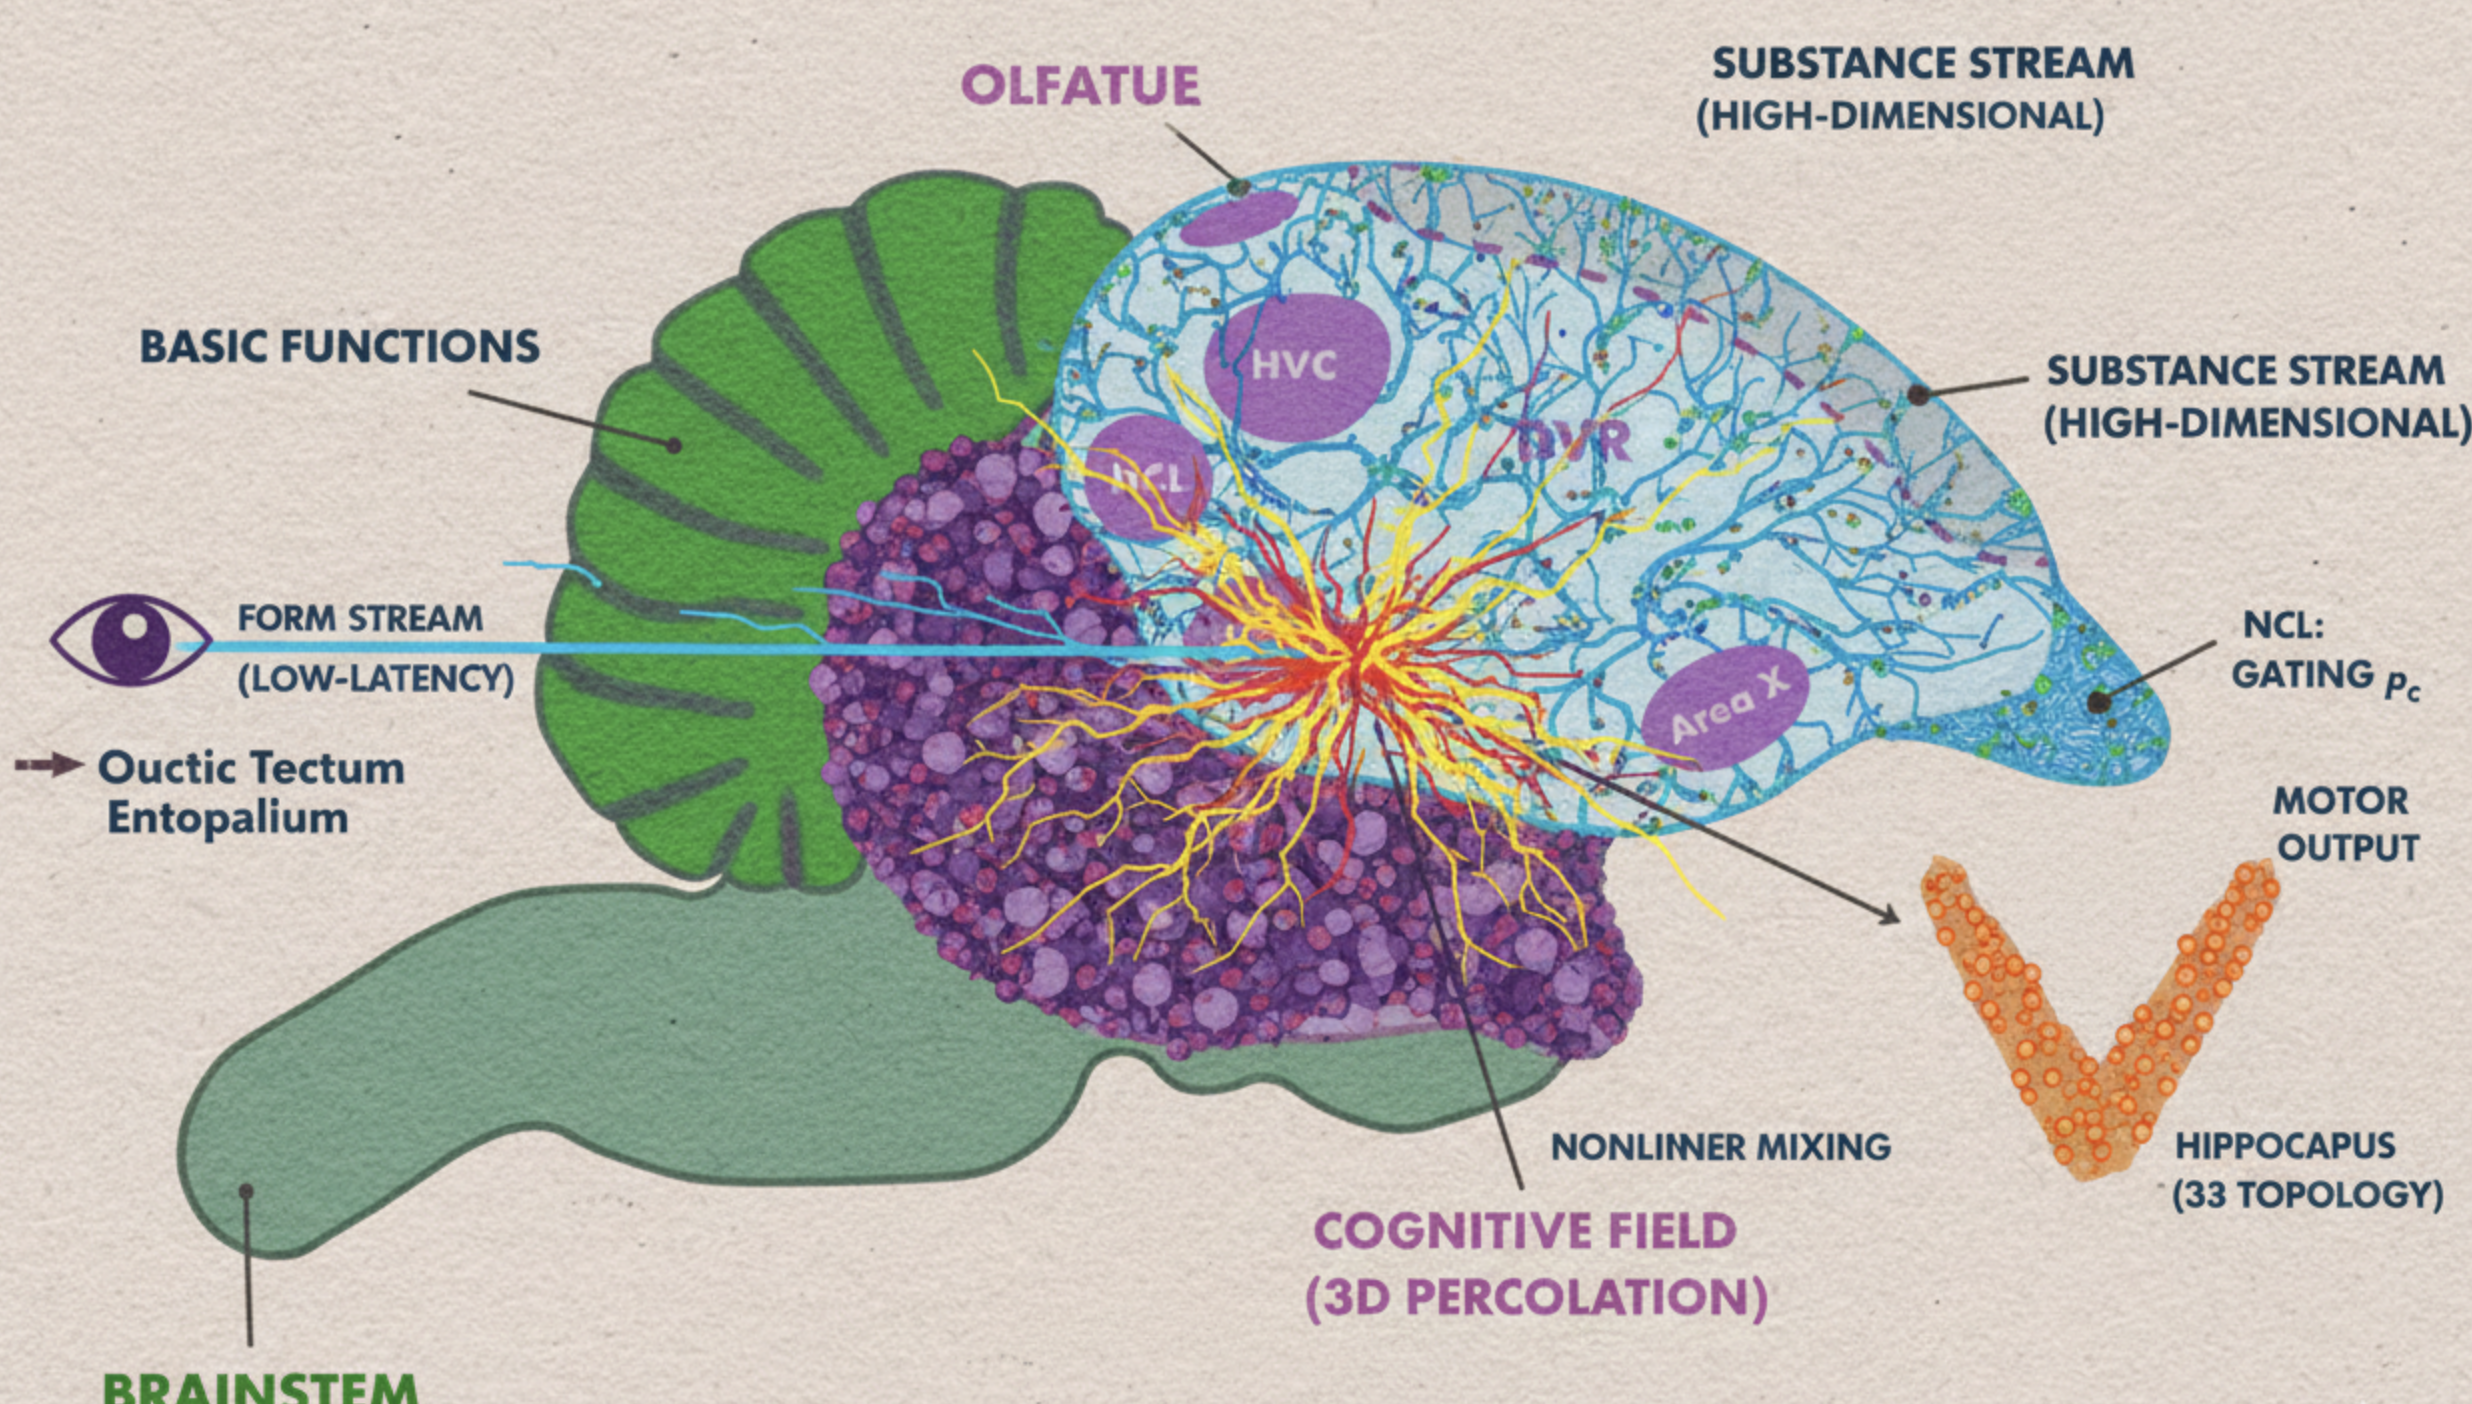
\includegraphics[width=0.96\linewidth,height=0.70\textheight,keepaspectratio]{image/birds.png}
    \caption{鸟类大脑示意图}
\end{figure}

\begin{itemize}
    \item   \textbf{位置细胞 (Place Cells)}：在乌鸦脑中，这些细胞不是分布在层状切片上，而是分布在 \textbf{V 形的 3D 结构} 中。
    \item   \textbf{本理论框架视角}：这是一个 \textbf{高维索引表 (Hash Map)}。由于 3D 邻域连接更丰富，乌鸦的海马体在单位体积内能存储的 \textbf{拓扑锚点 (Topological Anchors)} 密度远高于人类。
    \item   \textbf{度量张量 ($g_{\mu\nu}$)}：人类的度量是\textbf{欧氏}的（Grid Cells 铺路）。乌鸦的度量似乎是\textbf{图论}的。它更关注“地标之间的拓扑连接”而非绝对距离。这使得 $G_W$（世界图）极其紧凑，检索速度极快。
\end{itemize}



\smalltitle{认知场 ($\Psi$)：Nidopallium (新纹状体) 的逾渗动力学}

这是乌鸦智能的核心——\textbf{DVR (背侧室脊)}，特别是 \textbf{Nidopallium (新纹状体)}。它不是皮层，它是一团 \textbf{高密度的神经毡 (Neuropil)}。
\begin{itemize}
    \item \textbf{\textcolor{structurecolor}{物理介质：3D 晶格 (3D Lattice)}}
    \begin{itemize}
        \item   神经元不是排列成列，而是聚集成 \textbf{簇 (Clusters)}。
        \item   \textbf{连接拓扑}：\textbf{小世界 + 3D 网格}。任意两个神经元之间的突触跳数极少。
        \item   \textbf{场方程修正}：思维流 $\Psi$ 的传播不再遵循波动方程，而是遵循 \textbf{逾渗方程 (Percolation Equation)}：
            $$ P(p) \propto (p - p_c)^\beta $$
        \begin{itemize}
            \item   \textbf{$p$}：突触激发的概率。
            \item   \textbf{$p_c$}：临界阈值。
        \end{itemize}
    \end{itemize}

    \item \textbf{\textcolor{structurecolor}{动力学形态：受控雪崩 (Controlled Avalanche)}}
    \begin{itemize}
        \item   人类思维像 \textbf{水波}（干涉、衍射）,乌鸦思维像 \textbf{闪电}（击穿、分支）,当一个语义子（如“闪光的物体”）被激活，它会在高密核团中引发一次 \textbf{局部雪崩}。
        \item   \textbf{优势}：\textbf{极速相变}。系统可以在 $\Delta t \to 0$ 的时间内，从“静止”切换到“全脑激活”。这是为了适应飞行生存所需的毫秒级决策。
    \end{itemize}
\end{itemize}



\smalltitle{宏观层 ($L_{macro}$)：NCL 的闸门控制}

\textbf{NCL (尾外侧原脑里)} 是鸟类的“前额叶 (PFC)”。但它不依靠长程抑制（因为没有长程白质束），而是依靠 \textbf{局部闸门 (Local Gating)}。
\begin{itemize}
    \item \textbf{\textcolor{structurecolor}{物理职能：调节临界点 ($p_c$)}}
    \begin{itemize}
        \item   NCL 向 DVR 的各个核团投射 \textbf{多巴胺 (DA)} 和 \textbf{GABA}。
        \item   \textbf{TCE 方程实现}：
            $$ \hat{\mathcal{O}}_{macro} \to \Delta p_c(\mathbf{r}) $$
        \begin{itemize}
            \item   \textbf{抑制}：提高临界阈值 $p_c$。雪崩被限制在局部（专注）。
            \item   \textbf{激发}：降低临界阈值 $p_c$。雪崩传遍全脑（联想/冲动）。
        \end{itemize}
    \end{itemize}

    \item \textbf{\textcolor{structurecolor}{工作记忆：核团内的混响 (Reverberation)}}
    \begin{itemize}
        \item   人类依靠皮层间的长程回路维持 WM, 乌鸦依靠 \textbf{核团内部的微回路 (Micro-circuitry)},信息在 NCL 的一个小簇内部反复回荡，形成一个 \textbf{高能量密度的孤立子}。
        \item   \textbf{能效比}：这种局部维持比全脑广播要节能得多。这也是乌鸦大脑体积小但效率高的原因。
    \end{itemize}
\end{itemize}


\smalltitle{比较物理学：人类 vs 乌鸦}


\begin{table}[htbp]
\centering
\begin{tabularx}{\textwidth}{l X X X}
\toprule
\rowcolor{structurecolor!20} 维度 & \textbf{人类 (Cortex / 2D)} & \textbf{乌鸦 (Nuclei / 3D)} & \textbf{物理隐喻} \\
\midrule
\textbf{拓扑结构} & \textbf{层流 (Laminar)} & \textbf{核团 (Nuclear)} & \textbf{书页 vs. 晶体} \\
\textbf{传播模式} & \textbf{波动 (Wave)} & \textbf{逾渗 (Percolation)} & \textbf{声波 vs. 闪电} \\
\textbf{连接介质} & \textbf{白质 (长程光纤)} & \textbf{灰质 (短程互联)} & \textbf{互联网 vs. 局域网} \\
\textbf{计算优势} & \textbf{全局抽象 / 符号逻辑} & \textbf{局部敏捷 / 物理因果} & \textbf{CPU vs. FPGA} \\
\textbf{宏观控制} & \textbf{全局广播 (Broadcasting)} & \textbf{局部闸门 (Gating)} & \textbf{中央集权 vs. 联邦调控} \\
\bottomrule
\end{tabularx}
\end{table}



\smalltitle{工程启示：AGI 的“乌鸦时刻”}


乌鸦的大脑解剖为 AGI 硬件指明了另一条道路——\textbf{不一定要模仿人脑皮层}。
\begin{enumerate}
    \item \textbf{3D-IC 堆叠 (3D Stacking)}：
    \begin{itemize}
        \item   未来的 AGI 芯片应模仿乌鸦的 \textbf{DVR 结构}，采用垂直堆叠的计算单元，利用 TSV（硅通孔）实现极短的物理连接。
        \item   这能大幅降低 \textbf{$E_{transfer}$ (传输能耗)}，提高 \textbf{$\kappa$ (耦合度)}。
    \end{itemize}

    \item \textbf{小世界硬件 (Small-World Hardware)}：
    \begin{itemize}
        \item   放弃全局共享内存（对应人类白质），采用 \textbf{分布式存内计算 (Cluster-based CIM)}。
        \item   每个计算核团（Expert）拥有独立的记忆和动力学，通过 \textbf{临界逾渗} 交换信息。
    \end{itemize}

    \item \textbf{专用化智能}：
    \begin{itemize}
        \item   如果人类是 \textbf{Type A (通用理智型)}，乌鸦就是 \textbf{Type B (敏捷战斗型)}。
        \item   对于自动驾驶、机器人控制等\textbf{强实时性、强物理交互}的任务，\textbf{乌鸦架构（3D核团+逾渗动力学）} 优于人类架构。
    \end{itemize}
\end{enumerate}
\textbf{总结}：乌鸦大脑可被视为 \textbf{本理论框架} 理论在 \textbf{高密度介质} 中的一类特解。它提示我们：只要满足 \textbf{“微观锚定、场介质、宏观控制”} 的三体架构，哪怕没有哺乳类式六层皮层结构，智能仍然可以通过 \textbf{阈值型群体激活（雪崩/临界态）} 的机制稳定涌现。



\section{章鱼 (The Octopus)：具身化的联邦式智能孤岛}
\label{sec:section_446}

如果说人脑是 \textbf{Type A (中央集权制)} 的巅峰，致力于构建一个统一的、全知的世界模型；那么章鱼则是 \textbf{Type C (松散联邦制)} 的极致，它证明了智能可以存在于\textbf{“多中心、弱耦合、异构化”}的拓扑结构中。

我们将章鱼不再视为一个拥有八条腿的生物，而是一个\textbf{“弱耦合的联邦式流体计算网络”}。它代表了智能演化树上与脊椎动物完全正交的另一条路径：在没有刚性骨架（几何约束弱）和统一中央大脑（宏观控制弱）的极端条件下，如何通过\textbf{形态计算}与\textbf{局部场自治}来解决无限自由度（Infinite DOF）的控制难题。在本理论框架的角度下看，章鱼是一个\textbf{“多体耦合振子系统”}。它的智能并非完全由中央神经系统计算得出，而是通过\textbf{物理身体的流变性（软体物理学）}与\textbf{局部神经场的自治性}，在\textbf{“形态-计算”}的界面上涌现。它是\textbf{“认知场 ($\Psi$)”}与\textbf{“物理场 ($\Omega$)”}边界最模糊的物种——\textbf{身体本身就是计算的一部分}。

\smalltitle{本节内容说明}
\begin{itemize}
    \item \textbf{“分布式”是结构事实，但不是完全去中心}：章鱼腕足神经系统强大且自治，但中央脑仍承担学习、目标选择与全局偏置；本文的 Type C 叙述应理解为“弱耦合多中心”，而非“无中央”。
    \item \textbf{身体图谱差异要避免绝对化}：章鱼缺乏脊椎动物式同源体表映射是常见观点，但“是否有体感表征/以何种方式存在”在不同研究范式下表述不同；本文此处强调的是“中央不维持高分辨率腕足坐标”。
    \item \textbf{形态计算=把约束下放到材料}：把控制问题降维的关键不在“算力更强”，而在材料/肌肉水静力骨骼提供的物理先验与被动稳定性。
\end{itemize}



\smalltitle{语义子解剖：异构语义与局部方言}


章鱼的语义子空间是\textbf{分块 (Partitioned)} 且 \textbf{异构 (Heterogeneous)} 的。中央脑与腕足脑“说”着不同的语言，二者之间不存在全局统一的度量张量。

\begin{figure}[htbp]
    \centering
    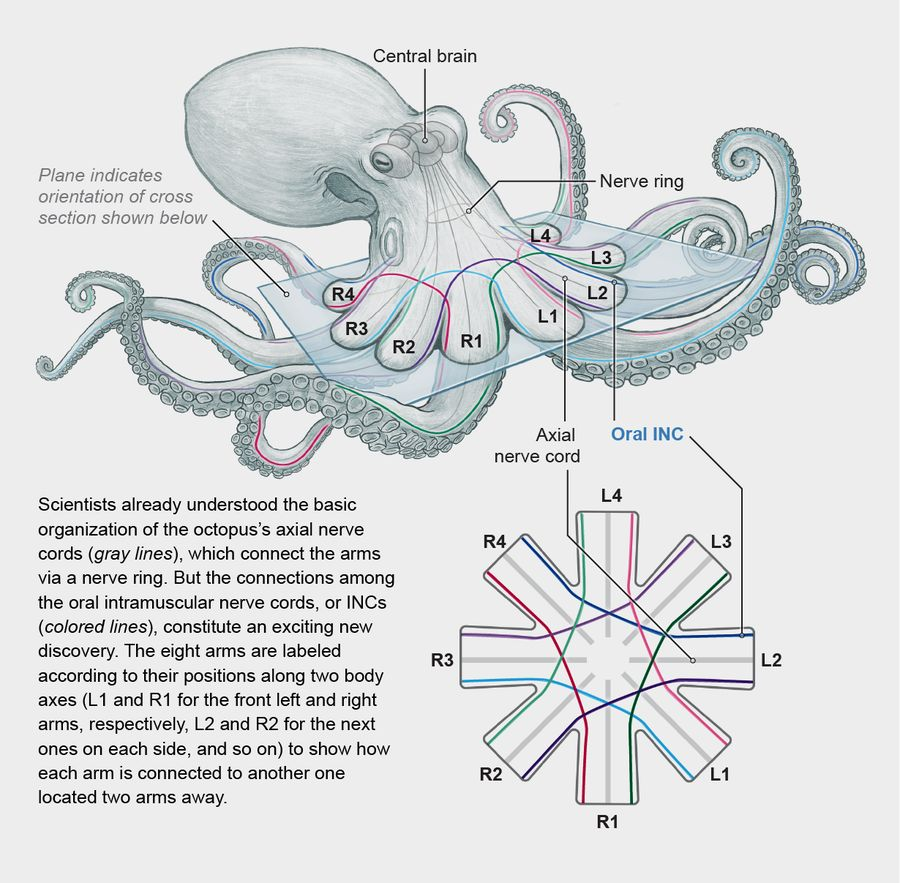
\includegraphics[width=0.96\linewidth,height=0.70\textheight,keepaspectratio]{image/octopus.jpg}
    \caption{章鱼的大脑结构示意图}
\end{figure}


\begin{itemize}
    \item   \textbf{中央语义子 ($\mathcal{S}_{central}$)}：
    \begin{itemize}
        \item   \textbf{类型}：\textbf{高阶视觉与长期记忆}。
        \item   \textbf{几何定义}：定义在 \textbf{视叶 (Optic Lobes)} 的流形上。
        \item   \textbf{内容 ($T_{sub}$)}：主要处理“威胁”、“猎物”、“地形”等全局对象。
        \item   \textbf{特征}：\textbf{稀疏且抽象}。更关键的是，它不以脊椎动物式的方式维持\textbf{高分辨率的腕足本体坐标}；中央更多处理“目标/情境”，而把大量连续控制留给腕足局部回路。
    \end{itemize}

    \item   \textbf{腕足语义子 ($\mathcal{S}_{arm}$)}：
    \begin{itemize}
    \item   \textbf{类型}：\textbf{接触式感知与局部运动}。
    \item   \textbf{几何定义}：定义在 \textbf{腕足神经索 (Brachial Cords)} 的圆柱形流形上。
    \item   \textbf{内容 ($T_{sub}$)}：包含“纹理”、“化学味觉（吸盘味觉）”、“局部弯曲度”。
    \item   \textbf{特征}：\textbf{致密且具身}。这是高频的物理交互信号。
    \end{itemize}

    \item   \textbf{交互协议}：\textbf{窄带意图传输}。中央与腕足之间的神经瓶颈极窄（轴突数量少），传输的不是 $T_{form}$（具体的运动轨迹 $\mathbf{x}(t), \dot{\mathbf{x}}(t)$），而是高度压缩的 \textbf{目标势能 ($V_{target}$)} —— 如：“去那里”、“抓那个”。
\end{itemize}



\smalltitle{架构映射：弱耦合的联邦拓扑}


章鱼的架构展示了 本理论框架中 \textbf{“多层场耦合 ($\kappa_{coupling} \to \text{Low}$)”} 的典型形态。系统依靠\textbf{局部自治}而非全局同步来维持运转。
\begin{enumerate}
    \item \textbf{宏观层 ($L_{macro}$)：中央脑 (Vertical Lobe) —— 弱协调者}
    \begin{itemize}
        \item   \textbf{物理职能}：\textbf{全局势能偏置 ($\mathbf{\Gamma}_{global}$)} 的设定者（可视为 $\mathbf{\Gamma}_{macro}$ 在 Type C 结构下的全局分量）。
        \item   \textbf{控制失效}：面对软体动物的 \textbf{无限自由度 (Infinite DOF)}，中央控制在数学上是 \textbf{不适定 (Ill-posed)} 的（算不过来）。因此，宏观层放弃了对微观动作的微操权。
        \item   \textbf{操作模式}：它仅向全系统广播一个 \textbf{模糊的目标场}（如“向右前方探索”）。这相当于在全局流形上设定了一个 \textbf{大致的引力方向}，而非具体的测地线。
    \end{itemize}

    \item \textbf{分布式认知场 ($\Psi_{total}$)：多中心流形}
    \begin{itemize}
        \item   \textbf{拓扑结构}：\textbf{星形-环形混合拓扑}。
            $$ \Psi_{total} = \Psi_{central} \oplus \sum_{i=1}^8 \Psi_{arm_i} $$
        \item   \textbf{中央场 ($\Psi_{central}$)}：负责视觉决策和学习。
        \item   \textbf{局部场 ($\Psi_{arm}$)}：每条腕足拥有独立的神经节（约5000万神经元），构成一个 \textbf{独立的谐振腔}。
        \item   \textbf{横向通信}：腕足之间通过 \textbf{神经环 (Interbrachial Commissure)} 进行直接通信，无需经过中央脑。这允许腕足在“大脑”不知情的情况下协调动作（如接力传递食物）。
        \item   \textbf{动力学}：\textbf{局部自治}。有实验观察表明，腕足在与中央脱耦后仍可在一定条件下独立完成“退缩”、“抓取”等局部动作。这支持 $\Psi_{arm}$ 具备相对独立的 \textbf{局部维持机制}（可类比局部工作记忆）与 \textbf{微观层反馈回路}。
    \end{itemize}

    \item \textbf{微观层 ($L_{micro}$)：吸盘与色袋 —— 智能蒙皮}
    \begin{itemize}
        \item   \textbf{物理职能}：\textbf{分布式反射控制器}（带感知-行动短回路）。
        \item   \textbf{吸盘 (Suckers)}：每个吸盘都有独立的神经节。它们不仅是传感器，还是微型的 \textbf{反射控制器}（自主决定抓紧或松开，甚至会拒绝抓取自身——一种局部的自我识别）。
        \item   \textbf{色素细胞 (Chromatophores)}：皮肤直接通过光感应进行变色（\textbf{皮肤视觉}）。这一过程绕过了大脑，是 \textbf{“感知-行动”在微观层直接短路} 的极致案例。
    \end{itemize}
\end{enumerate}




\smalltitle{动力学分析：形态计算与刚度波}


章鱼如何解决“控制面条去抓豆腐”的物理难题？本理论框架将其解释为 \textbf{形态计算 (Morphological Computation)} —— 利用物理定律代替逻辑运算。
\begin{itemize}
    \item \textbf{阶段 I：全局激发 (Global Excitation) —— 指令广播}
    \begin{itemize}
        \item   中央脑注入第三驱动力 $\vec{J}_{self}$，但这只是一个 \textbf{触发信号 (Trigger)}。
        \item   信号内容：\lstinline|Vector_Target| + \lstinline|Go|。
    \end{itemize}

    \item \textbf{阶段 II：形态相变 (Morphological Phase Transition) —— 刚度波}
    \begin{itemize}
        \item   腕足本质是 \textbf{液态} 的，难以精确控制。为了执行动作，腕足神经索会激发一种 \textbf{“刚度波” (Stiffening Wave)}。
        \item   \textbf{物理机制}：通过共收缩肌肉（Muscular Hydrostat），腕足在流体身体中临时构建出一个 \textbf{“伪关节” (Pseudo-Joint)}。
        \item   \textbf{本理论框架解释}：这是一种 \textbf{由信息驱动的物理相变}。认知场 $\Psi_{arm}$ 在局部区域瞬间 \textbf{结晶}，将无限自由度降维为有限自由度（类似人类的肘关节）,动作沿着这个临时的“晶体结构”传导，就像波沿着绳子传播。
    \end{itemize}

    \item \textbf{阶段 III：水库计算 (Reservoir Computing) —— 接触适配}
    \begin{itemize}
        \item   当腕足接触物体时，柔软的肉体自动适应物体的形状。
        \item   \textbf{无需计算}：这种适应不是算出来的，而是 \textbf{物理定律（材料力学）} 自动完成的。
        \item   \textbf{计算外化}：章鱼将计算负担 \textbf{卸载 (Offload)} 给了水的流体力学和自身的非线性弹性。\textbf{身体本身就是认知场的一部分（扩展流形）。}
    \end{itemize}
\end{itemize}


\smalltitle{比较物理学：人类 vs. 章鱼}


在本理论框架2.0 的智能相图中，人类与章鱼代表了两个正交的演化吸引子：

\begin{table}[htbp]
\centering
\begin{tabularx}{\textwidth}{l X X}
\toprule
\rowcolor{structurecolor!20} 维度 & \textbf{人类 (Human)} & \textbf{章鱼 (Octopus)} \\
\midrule
\textbf{拓扑架构} & \textbf{Type A (单极独裁)} \newline 强一致性，全局同步 & \textbf{Type C (松散联邦)} \newline 强鲁棒性，局部自治 \newline \\
\textbf{身体映射} & \textbf{完全映射} (Homunculus) \newline 大脑知道手在哪 & \textbf{无映射} (No Somatotopy) \newline 大脑不知道手在哪 \newline \\
\textbf{控制带宽} & \textbf{宽带} (脊髓含数百万轴突) \newline 精确位置控制 & \textbf{窄带} (视神经细，腕神经粗) \newline 模糊意图控制 \newline \\
\textbf{自由度 (DOF)} & \textbf{有限} (关节刚体) \newline 运动学方程可解 & \textbf{无限} (连续介质软体) \newline 运动学方程不可解 \newline \\
\textbf{计算策略} & \textbf{模型预测控制 (MPC)} \newline 在大脑中模拟物理 & \textbf{储水池计算 (Reservoir)} \newline 利用物理作为计算资源 \newline \\
\textbf{自我体验} & \textbf{统一的独白} (Monologue) \newline 只有一个“我” & \textbf{多声部的爵士乐} (Polyphony) \newline 可能是碎片化的、多焦点的意识流 \newline \\
\bottomrule
\end{tabularx}
\end{table}



\smalltitle{工程启示：软体机器人的 本理论框架 蓝图}


章鱼的架构为 AGI 在物理世界中的落地（具身智能）提供了关键指引，特别是针对非刚体机器人。
\begin{enumerate}
    \item \textbf{控制论的范式转移}：目前的机器人控制依然沿用“人类范式”（在 GPU 中精确计算关节角度）,这对于软体机器人是算力死路。
    \begin{itemize}
        \item   \textbf{本理论框架建议}：采用章鱼范式。中央模型只发 \textbf{意图 (Intention)} 和 \textbf{增益 (Gain)}，不发轨迹。
    \end{itemize}

    \item \textbf{边缘智能的物理化}：末端执行器必须具备 \textbf{高度自治的神经形态电路}。
    \begin{itemize}
        \item   利用 \textbf{柔性电子皮肤} 和 \textbf{智能材料}，在接触点直接完成物理信息的处理（微观屏蔽），只向上传递高阶语义（“抓住了”/“滑脱了”）。
    \end{itemize}

    \item \textbf{分布式算力的组织}：当 AGI 的规模大到无法单体容纳时，必须走向 \textbf{Type C (联邦)}。
    \begin{itemize}
        \item   章鱼证明了：\textbf{不需要全知全能的中央大脑，也能产生高级智能。} 关键在于设计好中央与边缘之间的 \textbf{“窄带语义协议”} —— 如何用最少的比特（形），指挥最复杂的物理操作（质）。
    \end{itemize}
\end{enumerate}

\begin{bquote}
    \textbf{本节结语}：

    章鱼告诉我们，智能不一定非要对抗物理（精确控制），也可以 \textbf{利用物理}（顺应形态）。在它的世界里，身体不是被操控的木偶，而是思维流动的河床。

    \textbf{真正的具身智能，是让算法流淌进材料里，让物理本身成为计算。}
\end{bquote}



\section{植物菌丝网络 (The Mycelial Network)：无头的水力经济流形}
\label{sec:section_4579}

如果说章鱼代表了动物界中\textbf{“联邦自治”}的极致，那么植物菌丝网络（Mycelial Network）则代表了生物界中最古老、最庞大的\textbf{“水力计算（Hydraulic Computing）”}原型。它是隐藏在地下的\textbf{“暗网”}，通过纯粹的物理场动力学，在没有神经元的情况下实现了生态系统尺度的资源调度与风险对冲。作为 \textbf{Class II (场致型群体)} 的宏大样本，菌丝网络展示了智能如何从\textbf{低雷诺数流体物理学}中涌现。它没有中央处理器（宏观层缺失），也没有离散的符号逻辑（语义子主要是模拟量）。它通过\textbf{液压-电化学耦合场}，将森林地下的资源分配问题转化为一个\textbf{多源多汇的最小流阻优化问题}。它是自然界中\textbf{“计算即传输 (Computation is Transport)”}的终极形态。

\smalltitle{本节内容说明}
\begin{itemize}
    \item \textbf{网络主体与边界}：现实系统往往是“真菌-植物-土壤微生物”的耦合网络；把它抽象为单一菌丝网络属于模型化，但应明确它的边界条件来自宿主与环境。
    \item \textbf{“经济交换”是有效描述}：碳/氮/磷交换可用自由能与化学势差刻画，但交易并非理性计算，更多是局部机制（运输蛋白、梯度、反馈）的涌现结果。
    \item \textbf{控制层级是分布式慢变量}：即使缺少中央大脑，也存在慢变量（资源储量、局部通量、菌根界面状态）形成的有效宏观约束；因此“无宏观层”应理解为“无集中式规划器”。
\end{itemize}

在本理论框架的智能谱系中，菌丝网络代表了 \textbf{Class II (场致型群体)} 向 \textbf{Class III (盖亚型)} 过渡的特殊形态。它缺少集中式中央处理器（显式宏观层缺失），符号的离散性也较弱（语义子以模拟量为主）。

它的智能本质是：\textbf{利用流体力学和反应扩散方程，在物理空间中直接求解“多源多汇资源分配”的变分极值问题。}



\smalltitle{语义子解剖：平流输运的实物张量}

在菌丝网络中，信息（Information）与物质（Matter）尚未发生解耦，语义子不是抽象的指针，而是实实在在的\textbf{物质波包}。

\begin{itemize}
    \item   \textbf{几何定义 ($\mathbf{r} \in \mathcal{M}_{soil}$)}：
    \begin{itemize}
        \item   \textbf{底流形}：由菌丝管网构成的 \textbf{1-复形 (Graph)} 嵌入在土壤的 \textbf{3-流形} 中。
        \item   \textbf{动态拓扑}：这个流形是\textbf{生长}的。$\partial_t \mathcal{M} \neq 0$。菌丝的生长就是在扩张流形的边界。
    \end{itemize}

    \item   \textbf{形质张量结构 ($\mathcal{S} = T_{form} \otimes T_{sub}$)}：
    \begin{itemize}
        \item   \textbf{形分量 ($T_{form}$)}：\textbf{流体动力学矢量}。包含：\textbf{静水压 ($P$)}、\textbf{流速 ($\vec{v}$)}、\textbf{管径 ($r$)}。

        \textit{作用}：它定义了物质传输的\textbf{测地线}（阻力最小路径）。

        \item   \textbf{质分量 ($T_{sub}$)}：\textbf{生物化学标量}。包含：\textbf{碳 ($C$)、氮 ($N$)、磷 ($P_{phos}$) 的浓度}，以及\textbf{同位素标记}。

        \textit{作用}：它是被传输的\textbf{负载}，也是交易的\textbf{货币}。

        \item   \textbf{特征}：\textbf{守恒流 (Conserved Current)}。

        不同于神经信号（可以复制/放大），菌丝语义子遵循 \textbf{连续性方程}：
        $$ \frac{\partial \rho}{\partial t} + \nabla \cdot (\rho \vec{v}) = S_{source} - S_{sink} $$
        这意味着：\textbf{计算必须伴随着物质的真实移动。}
    \end{itemize}
\end{itemize}



\smalltitle{架构映射：无头的双场耦合机}

菌丝网络没有单一的“自我”，它依靠两个物理场的\textbf{非线性耦合}来维持秩序。
\begin{enumerate}
    \item \textbf{慢场：水力压力场 (The Hydraulic Field, $\Psi_{hydro}$)}
    \begin{itemize}
        \item   \textbf{物理机制}：\textbf{渗透压驱动的体积流 (Osmotically driven bulk flow)}。
        \item   \textbf{动力学方程}：\textbf{达西定律 (Darcy's Law) 的生物版}。
            $$ \vec{J}_{flux} = -\frac{k}{\mu} A(\mathbf{r}) \nabla P(\mathbf{r}, t) $$
        \begin{itemize}
            \item   \textbf{$A(\mathbf{r})$}：管网截面积（流形的度量）。
            \item   \textbf{$\nabla P$}：压力梯度（驱动力）。
        \end{itemize}
        \item   \textbf{智能体现}：\textbf{模拟计算 (Analog Computing)}。网络自动寻找压力梯度最大的路径,这等价于在几何上求解 \textbf{最小流阻路径 (Least Resistance Path)}。
    \end{itemize}

    \item \textbf{快场：生物电场 (The Bio-Electric Field, $\Psi_{elec}$)}
    \begin{itemize}
        \item   \textbf{物理机制}：\textbf{类动作电位 (Action Potential-like Spikes)}。当菌丝尖端遭遇捕食者或剧烈环境变化时，膜电位去极化，产生速度约为 $1 \sim 10 \, mm/s$ 的电波。
        \item   \textbf{动力学功能}：\textbf{全网广播与门控}。电信号不携带物质，但它携带\textbf{控制信息}。
        \item   \textbf{效应}：电波传导至某一区域，瞬间改变该区域的\textbf{离子通道通透性}，从而\textbf{阻断或加速}水力场的流动。
        \item   \textit{本理论框架解释}：\textbf{快场是慢场的“规范场 ($\mathcal{A}_\mu$)”}。电场修改了水力场的边界条件。
    \end{itemize}

    \item \textbf{符号澄清}：此处 $\Psi_{hydro}$ 与 $\Psi_{elec}$ 表示\textbf{物理场变量}，与前文作为“认知旋量场”的 $\Psi$ 不是同一层级概念。

    \item \textbf{3. 微观层 ($L_{micro}$)：菌丝尖端 —— 探索型 VTE}
    \begin{itemize}
        \item   \textbf{VTE 机制}：\textbf{顶端生长 (Apical Growth)}。尖端拥有极高密度的囊泡和受体。
        \item   \textbf{输入}：土壤中的化学梯度 $\nabla C_{nutrients}$。
        \item   \textbf{输出}：流形的延伸矢量 $\vec{v}_{growth}$。
        \item   \textbf{物理本质}：\textbf{将外部的化学势能转化为内部的几何长度}。
    \end{itemize}
\end{enumerate}


\smalltitle{宏观动力学：涌现的“看不见的手”}

菌丝网络没有大脑（$L_{macro}$ 缺失），那么，是谁决定了“要把氮运给橡树而不是松树”？答案是：\textbf{热力学经济学 (Thermodynamic Economics)}。

\begin{figure}[htbp]
    \centering
    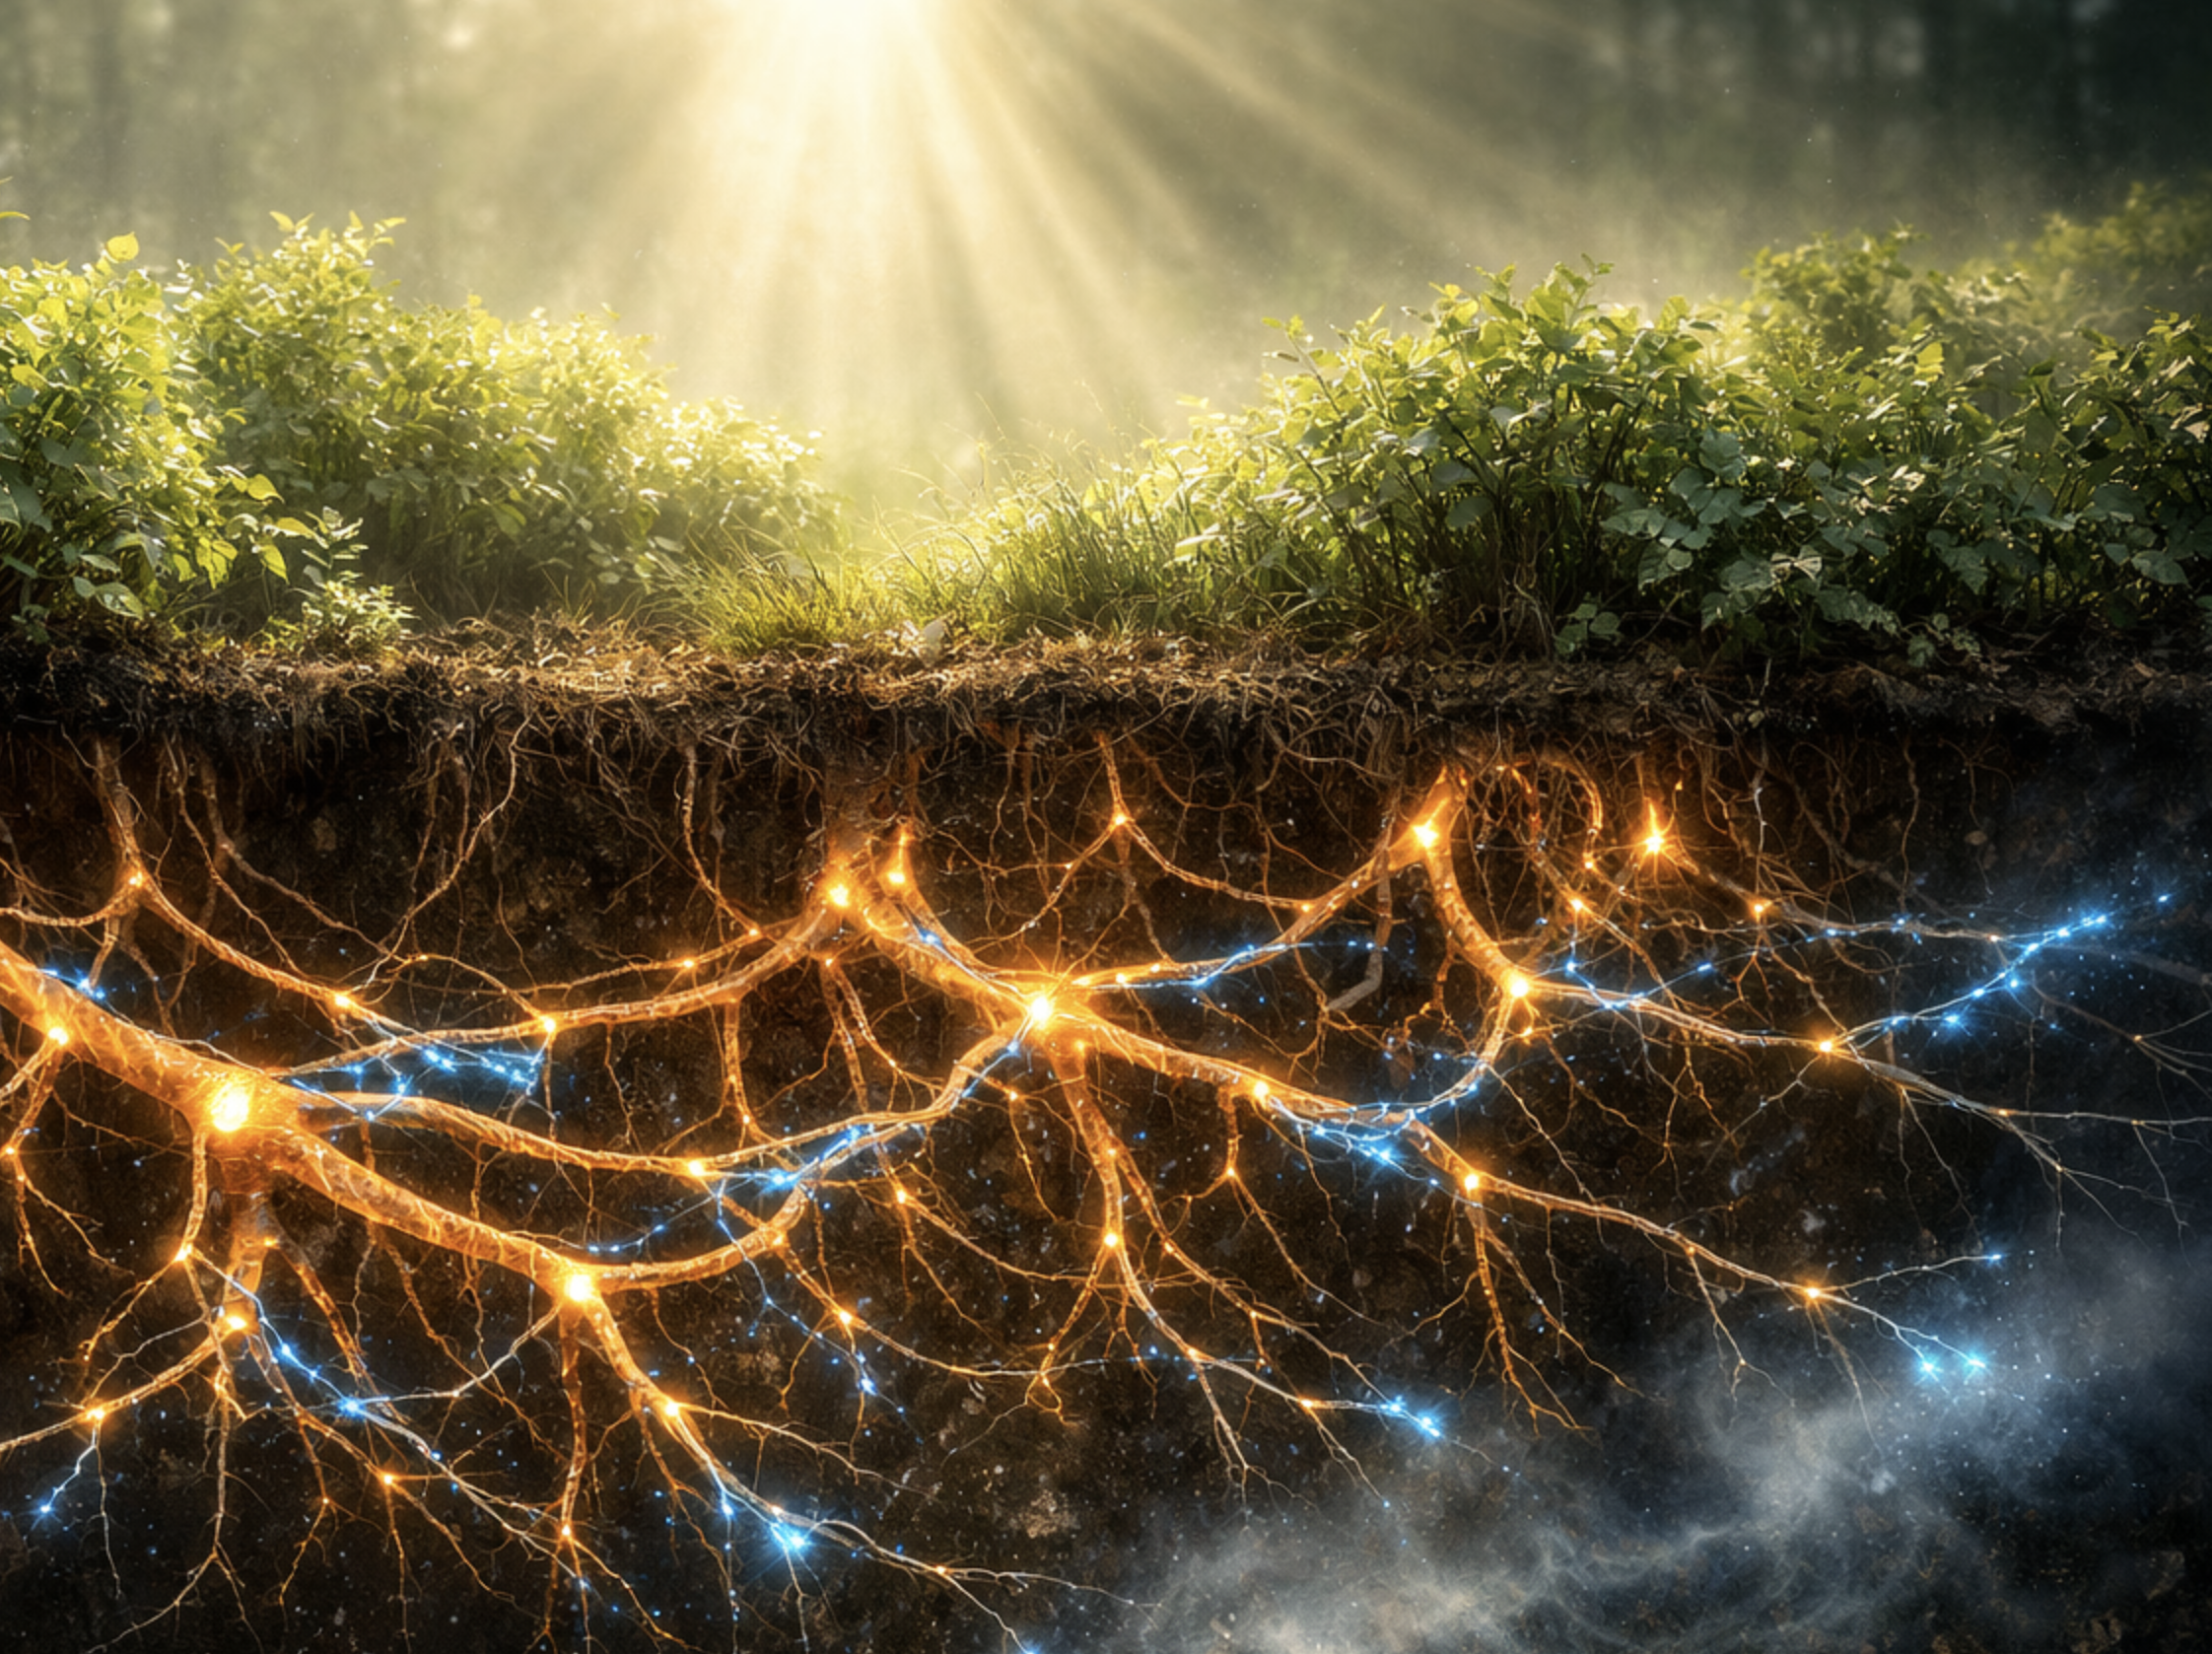
\includegraphics[width=0.82\linewidth,height=0.54\textheight,keepaspectratio]{image/plants.png}
    \caption{植物菌丝网络图示}
\end{figure}

\begin{enumerate}
    \item \textbf{交易机制：界面的阻抗匹配}, 在菌根界面（Arbuscules），真菌与植物根系进行物质交换。
    \begin{itemize}
        \item   \textbf{交换方程}：
        $$ \text{Rate}_{exchange} \propto \exp\left( -\frac{\Delta G_{trade}}{k_B T} \right) $$
        如果植物提供的碳（糖）多，真菌提供的磷少，\textbf{化学势差 ($\Delta \mu$)} 增大，通量自动增加。
        \item   \textbf{市场涌现}：真菌网络会自动从“出价低”（给糖少）的植物那里撤回菌丝，向“出价高”的植物增生菌丝。这不需要计算，这是\textbf{自由能最小化}的必然结果。
    \end{itemize}

    \item \textbf{拓扑优化：斯坦纳树的物理逼近}, 网络结构随时间演化，遵循 \textbf{耗散极小原理}：
    $$ \mathcal{L}_{net} = \int \left( \underbrace{R_{hydro} \|\vec{J}\|^2}_{\text{运输功耗}} + \underbrace{\lambda \cdot \text{Vol}(\mathcal{M})}_{\text{维护成本}} \right) dt $$
    \begin{itemize}
        \item   \textbf{初期}：高维、冗余的网状结构（探索）。
        \item   \textbf{后期}：\textbf{索流 (Cords)} 形成。常用的路径变粗（流导 $G \uparrow$），不用的路径萎缩断裂。
        \item   \textbf{结果}：演化出了近似 \textbf{斯坦纳树 (Steiner Tree)} 的极简拓扑。
    \end{itemize}
\end{enumerate}



\smalltitle{动力学特质：脉冲振荡作为“认知退火”}

菌丝网络内部观察到神秘的 \textbf{双向脉冲振荡 (Pulsatile Oscillation)}，这在本理论框架中被解释为一种 \textbf{主动的相变控制}。
\begin{itemize}
    \item   \textbf{现象}：流体并非稳恒流动，而是像呼吸一样前后震荡，叠加净流速。
    \item   \textbf{物理功能}：\textbf{防止死锁与混合}。在复杂的迷宫（土壤）中，单纯的梯度下降容易陷入局部极小值（死路）。
    \item   \textbf{振荡 ($T_{osc}$)} 提供了额外的动能，帮助物质\textbf{越过几何障碍}，并防止管道堵塞,这相当于在流形上施加了一个 \textbf{交流电压 (AC Voltage)}，维持系统的 \textbf{遍历性 (Ergodicity)}。
\end{itemize}



\smalltitle{总结与工程启示：湿件的智慧}

\begin{table}[htbp]
\centering
\begin{tabularx}{\textwidth}{l X X}
\toprule
\rowcolor{structurecolor!20} 维度 & \textbf{人脑 (Class V)} & \textbf{菌丝网络 (Class II+)} \\
\midrule
\textbf{介质} & 电化学驻波 (高频) & 水力-物质流 (低频) \\
\textbf{语义子} & 稀疏编码向量 (虚拟) & 实体物质包 (真实) \\
\textbf{控制} & 集中式宏观意志 & 分布式热力学平衡 \\
\textbf{逻辑} & 符号推理 & 物理模拟 \\
\textbf{优势} & 抽象、规划、速度 & 鲁棒、可扩展、能效比 \\
\bottomrule
\end{tabularx}
\end{table}

\textbf{对 AGI 的启示：}
菌丝网络展示了 \textbf{“无脑智能”} 的极限。对于未来的 \textbf{基础设施型 AI (Infrastructure AI)} —— 如城市电网、物流网络、星际通信网 —— 我们不需要一个巨大的中央大脑（那会导致计算瓶颈和单点故障）。
我们需要学习菌丝：
\begin{enumerate}
    \item \textbf{让数据包（语义子）携带物理属性（形质张量）}；
    \item \textbf{利用网络的局部物理定律（如拥塞控制协议的变种）}；
    \item 让全局的最优解通过 \textbf{局部势能的梯度滑行} 自动涌现。
\end{enumerate}
\textbf{菌丝网络是地球上最大的“流体计算机”，它证明了：只要物理定律被正确编织，泥土也可以思考。}
